\documentclass{uvamscse}

\usepackage{color}
\usepackage[usenames,dvipsnames]{xcolor}
\usepackage{url}
\usepackage{amsmath}


\usepackage{epigraph}
\setlength\epigraphwidth{8cm}
\setlength\epigraphrule{0pt}

\usepackage{etoolbox}
\makeatletter
\patchcmd{\epigraph}{\@epitext{#1}}{\itshape\@epitext{#1}}{}{}
\makeatother

\usepackage{listings}

\lstdefinelanguage{sdf}{%
  numbers=none,
  morekeywords={module,imports,exports,sorts,context,lexical,free,syntax,==,=,+,-,left,cons,prefer,avoid,bracket},
  columns=flexible,
  morestring=[b]",
  basicstyle=\footnotesize\mdseries,
  literate={->}{{\,\,$\to$\,\,}}1
}

\lstdefinelanguage{dcg}{%
  numbers=none,
  morekeywords={},
  morestring=[b]",
  basicstyle=\footnotesize\mdseries,
  columns=flexible,
}

\lstdefinelanguage{prolog},
  literate={:-}{{\,$\Leftarrow$\,\,}}1 {-->}{{$\to$\,}}1
}

\lstdefinestyle{mono}{
  basicstyle=\footnotesize\ttfamily
}

\lstdefinestyle{monosmall}{
  basicstyle=\footnotesize\ttfamily
}

\lstdefinelanguage{javascript}{
  keywords={typeof, new, true, false, catch, function, return, null, catch, switch, var, if, in, while, do, else, case, break},
  keywordstyle=\color{blue}\bfseries,
  ndkeywords={class, export, boolean, throw, implements, import, this},
  ndkeywordstyle=\color{darkgray}\bfseries,
  identifierstyle=\color{black},
  sensitive=false,
  comment=[l]{//},
  morecomment=[s]{/*}{*/},
  commentstyle=\color{purple}\ttfamily,
  stringstyle=\color{red}\ttfamily,
  morestring=[b]',
  morestring=[b]"
}

\lstdefinelanguage{json}{
    basicstyle=\normalfont\ttfamily,
    numbers=left,
    numberstyle=\scriptsize,
    stepnumber=1,
    numbersep=8pt,
    showstringspaces=false,
    breaklines=false,
    % frame=lines,
    backgroundcolor=\color{white},
    literate=
     *{0}{{{\color{black}0}}}{1}
      {1}{{{\color{black}1}}}{1}
      {2}{{{\color{black}2}}}{1}
      {3}{{{\color{black}3}}}{1}
      {4}{{{\color{black}4}}}{1}
      {5}{{{\color{black}5}}}{1}
      {6}{{{\color{black}6}}}{1}
      {7}{{{\color{black}7}}}{1}
      {8}{{{\color{black}8}}}{1}
      {9}{{{\color{black}9}}}{1}
      {:}{{{\color{black}{:}}}}{1}
      {,}{{{\color{black}{,}}}}{1}
      {\{}{{{\color{black}{\{}}}}{1}
      {\}}{{{\color{black}{\}}}}}{1}
      {[}{{{\color{black}{[}}}}{1}
      {]}{{{\color{black}{]}}}}{1},
}

\lstset{%
  frame=none,
  xleftmargin=2pt,
  stepnumber=1,
  numbers=left,
  numbersep=7pt,
  numberstyle=\ttfamily\scriptsize\color[gray]{0.3},
  belowcaptionskip=\bigskipamount,
  captionpos=b,
%  escapeinside={*'}{'*},
  % language=fl,
  tabsize=2,
  emphstyle={\bf},
  stringstyle=\itshape,
  showspaces=false,
  keywordstyle=\bfseries\rmfamily,
  columns=flexible,
  basicstyle=\small\mdseries,
  showstringspaces=false,
}

\newcommand{\cmd}[1]{\texttt{$\backslash$#1}}

\usepackage{graphicx}
\graphicspath{ {figures/} }

% \usepackage{polski}
\usepackage[utf8]{inputenc}
% \usepackage[applemac]{inputenc} % for Macs
\DeclareUnicodeCharacter{00A0}{ }
\usepackage[T1]{fontenc}
\usepackage{lmodern}

%%%%%%%%%%%%%%%%%%%%%%%%%%%%%%%%%%%%%%%%%%%%%%%%%%%%%%%%%%%%%%%%%%%%%%%%%%%%%%%%
% Title page.
%%%%%%%%%%%%%%%%%%%%%%%%%%%%%%%%%%%%%%%%%%%%%%%%%%%%%%%%%%%%%%%%%%%%%%%%%%%%%%%%

\title{Geographically-aware scaling for real-time persistent WebSocket applications.}
\coverpic[100pt]{figures/logo.png}
\subtitle{Master's Project in Software Engineering}
\date{Summer 2015}

\author{Łukasz Harężlak}
\authemail{lukasz.harezlak@gmail.com}
\host{Instamrkt, \url{https://instamrkt.com}}

\abstract{
  As the globalization of the world progresses, so does the globalization of web platforms and applications. Clients are expected to connect to the same system and generate and receive data in \textit{real time} (as close to the speed light limits as possible).

  The host company intends to have their cloud-based system as close to the physical and hardware limits as possible. A solution that satisfies latency, resource utilization and running cost criteria is sought for.

  In this research, I proposed three different architecture decompositions with varying degrees of geographical distribution. A cloud-based load test suite was designed to generate load used to benchmark 3 different architectures. Metric collection has been implemented for both client and server machines  (also real-time monitoring for the servers) and analysis of the metrics has been performed using scalability meters derived from scientific literature \cite{Models}.

  Research questions concern the geographic distribution of users and their proximity to WebSocket servers. The hypothesis is that when they are close, their experienced latencies and general system performance can be improved. According to some system limitations that cannot be easily overcome (not fully asynchronous database connectivity), the hypothesis has been refuted.
}

\begin{document}
\maketitle

%%%%%%%%%%%%%%%%%%%%%%%%%%%%%%%%%%%%%%%%%%%%%%%%%%%%%%%%%%%%%%%%%%%%%%%%%%%%%%%%
% Let the juicy stuff start.
%%%%%%%%%%%%%%%%%%%%%%%%%%%%%%%%%%%%%%%%%%%%%%%%%%%%%%%%%%%%%%%%%%%%%%%%%%%%%%%%

%%%%%%%%%%%%%%%%%%%%%%%%%%%%%%%%%%%%%%%%%%%%%%%%%%%%%%%%%%%%%%%%%%%%%%%%%%%%%%%%
\chapter{Introduction}

\epigraph{"Does this solution scale?"}{--- Every business person ever}

Everyone these days, probably more than ever, wants to build solutions that scale. Together with the globalization of our lives and businesses grows the need for global, distributed, scalable software systems.

To address this needs, more and more providers offer Cloud Computing solutions \ref{Cloud Scalability}, giving rise to the new architecture model called \textit{Infrastructure as a Service (IaaS)}. This makes building scalable software systems easier, since the system engineers do not have to design and maintain their proprietary server infrastructure anymore. This also allows to build systems that are more efficient in terms of resource usage - the existing \textit{IaaS} solutions offer scaling up and down capabilities in response to changes in demand for system's services.

As more and more systems are deployed to the cloud, a need for measuring their properties becomes more and more ubiquitous.

In order to reason about scalability-related properties of the system, one needs to define this notion considered by many as vague. For reasoning about cloud scalability, I find the following definition most relevant:

\begin{quote}
\cite{WeinstockOnSystem2006} Scalability is an ability of a system to handle increased workload by repeatedly applying a cost-effective strategy for extending a system capacity.
\end{quote}

Furthermore, to have a scientific discussion about scalability, quantifiable models and metrics are necessary. Selection of an appropriate scalability measurement model was a big part of my initial study.

\section{Initial Study}

Initial study pointed me to the relevant scalability vectors discussed by researchers and engineers regarding cloud computing. Each of them has a dedicated section in the Background Chapter \ref{Scalability}:

\begin{itemize}
  \item General Cloud Scalability (\ref{Cloud Scalability})
  \item Data Layer Scalability (\ref{Data Layer Scalability})
  \item WebSocket Scalability (\ref{WebSocket Scalability})
\end{itemize}

The study yielded multipile scalability measurement models. I analyzed the work of Jogalekar and Woodside \cite{EvaScaDS}, Srinivas and Janakiram \cite{SriJan}, Cooper et al. \cite{Ycsb} and multiple others.

Some of the proposed models are note applicable since they were designed for different types of scalability - not for a cloud-based distributed system, but for instance for multiprocessor or multi-threading scalability.

The models I selected to use for measurements in this research were proposed by Pattabhiraman et al. \cite{Models}. They were designed specifically for the task I am performing - measuring properties of a distributed system deployed in a cloud environment. Their models are also customizable - one can plug in metrics one deems relevant, which allowed us to select metrics that are representative of the business goal of the System Under Test \ref{The System Under Test}.

Selection and application of literature-based models is described in full in Scalability Measurements chapter \ref{Scalability Measurements}.

\section{Problem Statement}\label{Problem Statement}

The problem that I study in this research concerns application stack decomposition of the System Under Test \ref{The System Under Test}. It can be generalized to scalability of systems with similar characteristics:

\begin{itemize}
  \item utilizing real-time, uncacheable data,
  \item utilizing user-generated data,
  \item broadcast to user base distributed globally,
  \item broadcast using the WebSocket protocol \ref{WebSocket Protocol},
  \item deployed in the cloud,
  \item dynamically scalable (up and down).
\end{itemize}

This regards the size and geographical placement of WebSocket server instances, database and cache server instances (with data distribution), routing between them and internal layer communication.

I propose and compare three architectures \ref{Compared Architectures} to find which satisfies scalability criteria best.

More specifically, the host company is in need of scaling their system. The initial research showed little indication of which architecture decomposition will provide lowest client-experienced latencies, best allocated resources utilization and lowest operating cost. On top of that, they do not posses any tools or frameworks that would allow them to measure their system internally and externally. Neither are they in possession of a framework to generate the load test on which the scalability of the system could be measured.

\subsection{Research Questions}\label{Research Questions}
\begin{enumerate}
  \item What's the architecture decomposition stack that:
    \begin{enumerate}
      \item guarantees data delivery to geographically distributed users with minimal, consistent and manageable latency?
      \item scales up and down most effectively in response to demand changes?\footnote{This proved to be untestable as the researched progressed, because of the nature of DNS protocol, described in detail \ref{Excluded Metrics}.}
      \item guarantees lowest cost and best degree of utilization of the employed resources within a data center?
    \end{enumerate}
  \item Does architecture with geographical awareness of its users' distribution provide better Quality of Service than the baseline architecture?
\end{enumerate}

The answer to these questions is sought among the 3 tested architecture, described in detail later \ref{Compared Architectures}. Answers to these questions are evaluated using the models and a set of metrics described in detail in a dedicated chapter \ref{Scalability Measurements}, section \ref{Selected Meters and Metrics}.

\subsection{Solution Outline}

In order to answer the Research Questions \ref{Research Questions}, a solution consisting of the following steps was developed:
\begin{enumerate}
  \item \texttt{Preparing the load test suite}. It is used to simulate geographical distribution of users and load they generate as well as to collect latency-related metrics of WebSocket handshakes and message delivery. Described in details in a Load Testing Framework section \ref{Load Testing}.
  % [TODO] diagram of the distributed load test suite
  \item \texttt{Preparing the metric collection suite}. It is used to collect data from the application servers. This consists of collecting Amazon's CloudWatch\footnote{\url{http://aws.amazon.com/cloudwatch/}} metrics and our custom metrics (e.g. process memory usage). Metric collection process is described in details in a dedicated section \ref{AWS Available metrics}.
  \item \texttt{Feeding the collected metric into scalability meters}.
  \item \texttt{Automatic scalability management}. This is performed using Amazon's CloudWatch Alarms\footnote{\url{http://docs.aws.amazon.com/AmazonCloudWatch/latest/DeveloperGuide/AlarmThatSendsEmail.html}} triggering Auto Scaling Groups \footnote{\url{http://aws.amazon.com/autoscaling/}} capacity changes. In order to include our custom metrics in orchestrating the scalability process, a module based on Amazon's Python library (Boto\footnote{\url{http://aws.amazon.com/sdk-for-python/}}) was built.
\end{enumerate}

The solution is used to generate realistic user load and benchmark the performance of the system in 3 different versions of varying geographic distributions \ref{Compared Architectures}.

\subsection{Research Method}\label{Research Method}
Software Engineering is a relatively difficult field to investigate. Most of the problems are of design (rather than pure scientific) nature. West Churchman coined a specific term for these kind of problems \cite{Wckd}. He calls them \texttt{wicked}, since they are resistant to resolutions.

Easterbrook et al. \cite{EastBr} claim it is often difficult to identify the true underlying nature of the research problem and thus the best method to research it. In their work, they name and compare five most common classes of research methods to select from:
\begin{itemize}
  \item controlled experiments,
  \item case studies,
  \item survey research,
  \item ethnographies,
  \item action research.
\end{itemize}
They help to select the method by first establishing the type of research question being asked:
\begin{itemize}
  \item existence question - \textit{Does X exist?},
  \item description and classification question - \textit{What is X like?},
  \item descriptive-comparative question - \textit{How does X differ from Y?}.
\end{itemize}
The questions of this research are of the last type. The authors \cite{EastBr} suggest pinpointing up-front what will be accepted as a valid answer to the research question. I answer this question in a separate section \ref{Expected Answers}.

The detailed description of each of the methods helped me to settle for the \texttt{controlled experiment} as a research method for this research. It is well-suited for testing a hypothesis where manipulating independent variables has an effect of dependent ones, which is exactly the case of my research. The manipulated variable is architecture decomposition, and the measured ones are determined by scalability measurement models described in Scalability Measurements \ref{Scalability Measurements} chapter.

\subsection{Research Difficulty}
The experiments is performed in a shared cloud environment, which is inherently unpredictable and changing. Non-deterministic network conditions play a significant role here. Aside from that, one has to acknowledge the fact that control over hardware in a cloud environment is by definition given up by the researcher.

Designing and executing a test, yielding statistically relevant results, where all the necessary variables are controlled (within reasonable boundaries) is a huge challenge. Bornholt \cite{BornBen} mentions that even the linking order in the process of generating binaries can have an effect of the performance of the benchmarked system!

The focus of the project is on scaling a WebSocket application. This is a relatively new technology, thus finding proper scientific coverage is not trivial.

Some of the necessary development and data collection tools are relatively low-level and require thorough understanding of UNIX operating systems, on which the servers are deployed. The same is applicable to tuning the operating system for optimal TCP-related performance \ref{Kernel tuning}.

Simulating the geo-location of clients with reasonable accuracy also proves problematic.

Overall, it’s a complex project requiring knowledge of multiple aspects of both hardware (TCP, WebSocket protocol, networks, operating system), software (architecture, cloud computing, data replication/sharding).

\subsection{Hypothesis}
The correct geographical decomposition of the stack of The System Under Test \ref{The System Under Test} can lead to improved performance in comparison with the Baseline Architecture \ref{Baseline Architecture}.

The geographically distributed architectures \ref{Proposed Architecture I} and \ref{Proposed Architecture II} should provide lower user-experienced request handling and broadcast latencies than the baseline architecture \ref{Baseline Architecture}. Some of the latencies that are unavoidable due to geographical global distances, in case of these architectures, can be pushed down to lower levels of the systems. This means that the data retrieval / synchronization can happen asynchronously, in the background, rather than synchronously on every user's request.


On the other hand, the distributed versions of the architecture add complexity in multiple system layers. Implications of these will probably increase the cost of system utilization (due to increased internal data transfer).

\section{Contributions}
The research will result in the following contributions:

\begin{enumerate}
  \item Architecture decomposition analysis for system's meeting the criteria described in the Problem Statement section \ref{Problem Statement}.
  \item Case Study on Amazon Web Services\footnote{\url{http://aws.amazon.com/}} and usability of their cloud stack for applications using WebSocket protocol.
  \item Open sourced pieces of code for:
  \begin{itemize}
    \item metrics collection (both from the load test suite and the servers),
    \item auto-scaling execution,
    \item constructing scalability models and populating them with collected metrics,
    \item remote execution of load tests on a fleet of client-simulating servers.
  \end{itemize}
  These are described in details in Experiment Deliverables section \ref{Experiment deliverables}.
\end{enumerate}

\section{Related Work}\label{Related Work}

There is two key papers this research is based on. First of them is \textit{Multi-Cloud Provisioning and Load Distribution for Three-Tier Applications} by Grozev and Buyya \cite{GroBuy}. The second one is \textit{SaaS performance and scalability evaluation in clouds} by Pattabhiraman et al \cite{Models}.

\subsubsection{Multi-Cloud Provisioning and Load Distribution for Three-Tier Applications}

In this work, the authors tackle the problem of deploying applications across multiple clouds while satisfying system's nonfunctional requirements (in their understanding, application deployed in Amazon's \textit{us-east-1} region and \textit{eu-west-1} region would be deployed to multiple clouds). They propose algorithms for resource provisioning and load distribution. They focus on resource utilization and cost and legal regulations regarding serving users and servers geographical location and include them in their algorithms.

In order to satisfy the requirements, the authors had to develop their own routing stack. Both Amazon's services involved in the routing process -- Route 53 \footnote{\url{http://aws.amazon.com/route53/}} and Elastic Load Balancing\footnote{\url{http://aws.amazon.com/elasticloadbalancing/}} -- do not consider application's regulatory requirements when selecting a data center site. Moreover, they do not consider the cost and degree of utilization of the employed resources within a data center.

This is how they perform cloud selection to serve a user:
\begin{enumerate}
  \item As a first step, the user authenticates with one of their entry point servers. At this point, the entry point has the user’s identity and geographical location (extracted from the IP address).
  \item As a second step, the entry point broadcasts the user’s identifier to the admission controllers of all data centers. They call this step \textit{matchmaking broadcast}.
  \item The admission controllers respond to the entry point whether the user’s data are present and if they are allowed (in terms of legislation and regulations) to serve the user. In the response, they also include information about costs within the data center.
  \item Based on the admission controller's responses, the entry point selects the data center to serve the user and redirects him or her to the load balancer deployed within it. The entry point filters all clouds that have the user’s data and are eligible to serve him or her. If there is more than one such cloud, the entry point selects the most suitable with respect to network latency and pricing. If no cloud meets the data location and legislative requirements, the user is denied service.
  \item After a data center is selected, the user is served by the Application Server and Database servers within the chosen cloud.
\end{enumerate}

Below I list most relevant takeaways from their work.

\begin{description}
  \item[Sticky Load Balancing] - it is a technique of load balancing that routes same users to the same backend server instances. They utilize it in their work - I cannot in this research. Amazon's stack does not offer sticky load balancing for protocols other than HTTP.
  \item[Cloud Server Instance Termination] - it is not beneficial to terminate a running VM ahead of its next billing time. It is better to keep it running until its billing time in order to reuse it if resources are needed again.
  \item[Cost Minimization] - this is not an automated feature cloud providers offer. Authors advice on how to include it in a cloud controlling stack. It is an important business goal in my research.
  \item[Latency Minimization and Approximation] - authors, just as myself, treat latency as one of the key objectives in the process of optimizing their cloud stack. They approximate latencies and users geographic location using tools PingER\footnote{\url{http://www-iepm.slac.stanford.edu/pinger/}} and GeoLite\footnote{\url{http://dev.maxmind.com/geoip/legacy/geolite/}}. PingER is used to approximate latencies between user and a cloud and GeoLite to map users IP addresses to geographical coordinates. In my research, I do not need to use tools like that since Amazon's stack offers this in sufficient capacity.
\end{description}

Why is this work relevant? The authors are attempting to solve the same problem - how to distribute and route users between multiple clouds given arbitrary conditions. They work with a similar technology stack as I do.

\subsubsection{SaaS performance and scalability evaluation in clouds}

Pattabhiraman et al realized that cloud computing and its measurement provides a new set of challenges when it comes to measuring performance, as opposed to measuring performance of traditional software systems. They list key points for measuring cloud applications - validating and ensuring the elasticity of scalability and evaluating utility service billings and pricing models. Both are important in my case. They raise an interesting question regarding the latter:

\begin{quote}
 How to use a transparent approach to monitor and evaluate the correctness of the utility bill based on a posted price model during system performance evaluation and scalability measurement?
\end{quote}

The authors divide the performance indicators into three groups and propose formal quantifiable meters for each of them:
\begin{enumerate}
  \item computing resource indicators (CPU, disk, memory, networks, etc.),
  \begin{itemize}
    \item Computing Resource Allocation Meter (CRAM),
    \item Computing Resource Utilization Meter (CRUM),
  \end{itemize}
  \item workload indicators (connected users, throughput and latency, etc.),
  \begin{itemize}
    \item System Load Meter (SLM),
  \end{itemize}
  \item performance indicators (processing speed, system reliability, availability)
  \begin{itemize}
    \item System Performance Meter (SPM).
  \end{itemize}
\end{enumerate}
They also propose model which allow to combine the above: System Capacity Meter (SCM), System Effective Capacity Meter (SEC), Effective System Scalability (ESS), and Effective Scalable Range (ESR). Values that are fed into these meters are customizable. The meters are described in detail in the Scalability Measurements chapter \ref{Scalability Measurements}.

Authors perform a case study with Amazon's AWS stack. The case study consists of performed tests and measurements taken on scaling up and scaling down their application. It provides some warnings for me to consider:
\begin{itemize}
  \item Cloud limitations need to be taken into account. For instance, memory usage data is not collectible from their server instances using their services.
  \item One needs to be aware of hidden costs that cloud providers excel at introducing.
  \item One needs pay attention to inconsistencies in performance and scalability data, especially data collected using third-party tools and.
\end{itemize}

More related work is described in the following chapter - Background \ref{Background}.

\section{Document Outline}
In this section I outline the structure of the thesis - all chapters with short summaries.

\begin{enumerate}
  \item \texttt{Background} - contains a short summary of the literature study. Describes researched work in the relevant fields \ref{Background}.
  \item \texttt{Benchmarking} - contains a description and guidelines regarding the benchmarking process, which constitutes a big part of this research. Lists typical benchmarking mistakes and what I do to avoid them \ref{Benchmarking}.
  \item \texttt{The System Under Test} - contains a description and guidelines regarding the benchmarking process, which constitutes a big part of this research. Lists typical benchmarking mistakes and what I do to avoid them \ref{The System Under Test}.
  \item \texttt{Experiment Outline and Design} - contains a description of the conducted experiment, its goals and deliverables \ref{Experiment Outline and Design}.
  \item \texttt{Scalability Measurements} - contains a description of literature-based scalability metrics and models. Lists the models and metrics selected for measurements in this research, as well as all metrics collectible from the AWS cloud environment \ref{Scalability Measurements}.
  \item \texttt{Experiment Implementation} - contains a full description of the compared architectures and cloud stack on which the research is performed, including the technological details \ref{Experiment Implementation}.
  \item \texttt{Experiment results} - contains the data collected in the experiments \ref{Experiment results}.
  \item \texttt{Conclusions and Evaluation} - contains a list of conclusions derived from the analysis of the experiment results and the evaluation of the experiment \ref{Conclusions and Evaluation}.
  \item \texttt{Further Work} - contains a description of relevant, testable variables I did not have enough time to cover in this research. \ref{Further Work}
\end{enumerate}

%%%%%%%%%%%%%%%%%%%%%%%%%%%%%%%%%%%%%%%%%%%%%%%%%%%%%%%%%%%%%%%%%%%%%%%%%%%%%%%%

%%%%%%%%%%%%%%%%%%%%%%%%%%%%%%%%%%%%%%%%%%%%%%%%%%%%%%%%%%%%%%%%%%%%%%%%%%%%%%%%
\chapter{Background}\label{Background}

\section{Scalability}\label{Scalability}

Scalability seems to be a notion that everyone intuitively grasps, but has difficulties when it comes to clear explanations. In my literature study I came across a few definitions, which might help with that, of which three can be found below:

\begin{quote}
~\cite{Williams04} Scalability is a measure of an application system’s ability to, without modification, cost-effectively provide increased throughput, reduced response time and/or support more users when hardware resources are added.
\end{quote}

\begin{quote}
\cite{WeinstockOnSystem2006} Scalability is an ability of a system to handle increased workload (without adding resources).
\end{quote}\label{x}
In light of this definition we would talk about a scalability failure if one of the following occurred:
\begin{itemize}
  \item Address space was exceeded,
  \item Memory was overloaded,
  \item Available network bandwidth was exceeded,
  \item etc.
\end{itemize}

\begin{quote}
\cite{WeinstockOnSystem2006} Scalability is an ability of a system to handle increased workload by repeatedly applying a cost-effective strategy for extending a system’s capacity.
\end{quote}
According to this definition, one could determine system scalability failure if a given resource got overloaded or exhausted an adding capacity to this resource would not result in a proportional ability to handle additional demand, e.g.:
\begin{itemize}
  \item an additional processor will not contribute to meeting the higher demand if handing of that processor entails an overhead).
  \item a newly added server instance might not contribute to handling a higher user demand if slows down the routing process.
\end{itemize}

\subsection{Scalability Trade-offs}
Scalability is generally desired in the software systems, yet, as all architectural software decisions come at a cost \cite{GerHeiBench}; one must be aware of the trade-offs usually associated with it. Weinstock and Goodenough \cite{WeinstockOnSystem2006} and Tsai et al. \cite{WeiTek} point these out:
\begin{itemize}
  \item performance and scalability (non-scalable system will often demonstrate degrading performance with increasing demand, but scalable systems require performance sacrifice on lower usage levels),
  \item cost and scalability (designing a system to be scalable up-front entails additional costs),
  \item operability and scalability (it is difficult for humans to operate large systems),
  \item usability and scalability (it may be possible to increase servable demand with limiting system's service scope - e.g. removing personalization and displaying generic, cacheable data),
  \item data consistency and scalability (higher scalability can be achieved if system allows for data inconsistencies).
  \item levels of scalability mechanisms and automated migration (automated migration has to be aware of every level of scalability mechanism; the more of them the more complex the migration),
  \item workload support and database access (different workloads need support for different database access mechanisms, such as row-oriented storages, column-oriented storages or hybrid approaches).
\end{itemize}

\subsection{Need for Scalability}

As the globalization and internetization progresses, more and more systems are expected to be capable of serving millions of globally distributed users. A single server instance often cannot live up to that task and thus application needs to be divided and distributed in multiple smaller chunks. This division happens on different application layers, and different parts of the system have to communicate and synchronize with each other.

In case of many software systems (the system under test \ref{The System Under Test} included), user traffic, and with it the need for system services and resources, varies significantly. A need to be able to scale up and down dynamically in response to traffic arises from this.

Huge parts of the internet are shifting towards real-time. This trend is giving rise to new technologies for exchanging messages between clients and servers in the client-server architecture. Traditionally, client would send a request to a server and receive a response. This is hugely inefficient when there is a need for continuous bidirectional exchange of messages. As an improvement, new mechanisms for server-client communication have been introduced recently \ref{Client-Server Communication Improvements} to enhance the process and reduce overhead. One of them - WebSockets - are a huge next step on this path, but introduce new challenges. One of them is scalability of applications which make use of this technology.

\subsection{Existing Approaches}
Scalability has been studied in parallel computing, distributed computing, databases, and service-oriented architectures (SOA) \cite{WeiTek}. Scalable design principles for application servers include: divide-and-conquer, asynchrony, encapsulation, concurrency, parsimony, system partitioning, service-based layered architecture, pooling and multiplexing, queuing and background processes, data synchronization, distributed session tracking, and intelligent load distribution.

There exist multiple scalability vectors for web applications. Different decompositions of application stack can be applied to achieve the goal of scalability. A few traditional approaches of tackling an issue like that exist already \cite{Akamai}:
\begin{description}
  \item[Scaling up.]
  Increasing volume of system allocated resources (a stronger machine, or with a better configuration, including more computing resource, more memory, higher disk bandwidth and larger disk space \cite{WeiTek}). As internet is unreliable and so called "middle-mile bottlenecks" exist, a web application end-user latency and throughput experience is not fully deterministic. Traffic levels fluctuate tremendously, so the need to provision for peak traffic levels means that expensive infrastructure will sit underutilized most of the time. It is easy to implement, but costly, even extremely when you start pushing at current hardware limits.\cite{Qvef} Because the resources of a single machine cannot be increased infinitely, and increase of the cost is not proportional to the increase of the resources, scale-up is not feasible in an Internet scale \cite{WeiTek}.
  \item[Scaling out.]
  Scaling out horizontally - increasing the number of units of resources comprising the system. Cost of hardware can be reduced dramatically this way. In a web application, one can deploy multiple instances of servers. Different types of balancing can be applied to distribute traffic among them: application layer balancing, business load balancing, and anticipating load. The overhead of parsing requests in the application layer is high thus limiting scalability compared to load balancing in the transport layer. Client state needs to be stored in a layer shared between the web servers.\cite{Qvef}  Scale-out is usually adopted in a cloud \cite{WeiTek}.
  \item[Content Delivery Networks.]
  These only handle static assets. Communication in our system \ref{The System Under Test} happens mainly over WebSockets, which are not supported by CDNs. CDNs can be divided into Big Data Center CDNs and Highly Distributed CDNs, which put application data within end-user ISPs.\cite{Akamai}
  \item[Peer to peer networks.]
  An architecture different from client - server, where users communicate with each other directly. It handles adding and removing nodes to and from the network dynamically very well.
\end{description}

\subsection{Scalability Factors}
There exist multiple scalability factors one has to be aware of when designing and implementing scalability of a software system\cite{WeiTek}.

\subsubsection{Levels of Scalability Mechanisms}
Most applications deployed in the cloud adopt a tiered application - typically the storage, application and presentation tiers. Cross-tier scaling is not very common because of the high cost of duplicating the whole application stack. Hybrid approach is more popular - the whole stack is duplicated but single tier scaling within the stack is leveraged.

Scalability mechanisms for each tier might be different, since each of them has its own intrinsic properties, objectives and constraints.

\subsubsection{Automated Migration}
For many systems, automatic migration of data is critical for scalability. This migration can be performed on-line (the application continuous operating throughout the whole process) or off-line (the application is taken down for maintenance).

\subsubsection{Workload Support}
Different workloads require different scalability mechanisms. On-line Analytical Processing (OLAP) applications have to be prepared to scale for high volume of read operations, whereas On-line Transaction Processing (OLTP) applications have to be prepared to scale for a lot of write operations. Mixed workloads (as is the case for The System Under Test \ref{The System Under Test}) require an architecture ensuring no biases towards either type of operations.

\subsubsection{Recovery and Fault-tolerance}
A scalable system needs to detect failures of nodes and scale down to exclude the failed node from operation. Similarly, when the failed node comes back to the system, it should scale up including the recovered node. In a fully scalable system, this process should be autonomous.

\subsubsection{Software Architecture}
In a scalable system, architecture should be divided into decoupled modules which can be scaled independently. Authors \cite{WeiTek} use Service-Oriented Architecture as a model example of an architecture that many scalable systems adopt.

\subsubsection{Database Access}
Accessing data is often time consuming. This is why data layer is likely to be a bottleneck of a SaaS application. Indirect access (accessing the data layer through an exposed API) allows data tier and other tiers to scale independently using their own preferred mechanisms.

\subsection{Cloud Scalability}\label{Cloud Scalability}
Cloud computing has become virtually ubiquitous. All biggest internet services are either deployed to a cloud, or run their proprietary cloud systems. A lot of companies running proprietary clouds also make them available for hosting to the external clients. Netflix\footnote{\url{https://aws.amazon.com/solutions/case-studies/netflix/}} and Spotify\footnote{\url{https://aws.amazon.com/solutions/case-studies/spotify/}} (both deployed to Amazon's AWS) are examples of the first approach, with Microsoft(Azure)\footnote{\url{https://azure.microsoft.com/}}, Google(Google Cloud Platform)\footnote{\url{https://cloud.google.com/}} and Amazon(Amazon Web Services)\footnote{\url{https://aws.amazon.com/}} being the example of the second. These services are typically billed on a resource utility basis.

General cloud capabilities and the cloud stack I am working with for the scope of this project is described in a dedicated chapter \ref{Cloud architecture setup}.

One of the biggest advantages of deploying one's architecture to the cloud that aforementioned companies offer is the ability to dynamically scale up and in response to application traffic changes.

As Grozev and Buyya \cite{GroBuy} put it, to fully facilitate cloud capabilities, software engineers need to design for the cloud, not only to deploy to it.

\subsection{Data Layer Scalability}\label{Data Layer Scalability}

Data layer scalability is an important part of system scalability. In a distributed system, multiple system agents share the data. There exist multiple strategies for operating on a shared, distributed data layer.

Data layer is often a performance bottleneck because of requirements for transactional access and atomicity - it is hard to scale out when system uses a relational data store \cite{GroBuy}.

\begin{description}
  \item[CAP Theorem]
  put forward by Eric Brewer \cite{Cap} states that it is impossible for a distributed system to provide all of the following guarantees:
  \begin{itemize}
    \item consistency,
    \item availability,
    \item partition tolerance.
  \end{itemize}
  Therefore, a trade-off needs to be made, depending on stakeholder priorities, which of the three to give up.
  \item[ACID]
   stands for Atomicity, Consistency, Isolation, Durability and is a set of properties guaranteeing reliable processing of database transactions. It has been a guideline in designing multiple database systems. The term was originally coined by Haerder and Reuter in 1983 \cite{ACID}.
  \item[BASE]
   stands for Basically Available, Soft State, Eventually Consistent \cite{EveCon}. It’s a complement of ACID. Author claims we lack precise metrics to measure BASE aspects and that is why every system implements eventual consistency differently.

  Most importantly for this research, the author \cite{EveCon} explains \textit{MySQL Cluster} - it performs much like an ACID database but with the performance benefits of a cluster. Aside from that, \textit{MySQL Replication} can be put to use. It can be configured at multiple topologies, not only the basic master-slave; consistency differs per configuration.
\end{description}

Many solutions and strategies for dealing with database scalability have emerged, including \textit{NoSQL} and \textit{NewSQL} databases, data replication and sharding \cite{Amza}.

Cooper et al touch on that subject in their work \cite{Ycsb}. They claim that in scaling out the database layer one should aim for elasticity (dynamically adding capacity to a running system) and high availability. These are hard to achieve using traditional database systems. They show that new protocols are being developed to address that issue, such as that: \textit{two-phase commit protocol} (provides atomicity for distributed transactions) and \textit{paxos}.


The authors \cite{Ycsb} also give an overview of different database systems, including \textit{PNUTS}, \textit{BigTable}, \textit{HBase}, \textit{Cassandra}, \textit{Sharded MySQL}, \textit{Azure}, \textit{CouchDB}, and \textit{SimpleDB}.


In their work \cite{Ycsb}, we can find enumeration of classic data-related scalability trade-offs:
\begin{itemize}
    \item read performance and write performance,
    \item latency and durability,
    \item synchronous and asynchronous replication,
    \item data partitioning (column and row-based storage).
  \end{itemize}


The technology stack I have been working with in the scope of this project consists of \textit{MySQL} as persistent storage and \textit{Redis} as a key-value cache. It is described in details in a dedicated chapter \ref{Technology Stack}.

\subsubsection{MySQL Scalability}

MySQL White paper \cite{MySQL} gives us a good overview of how scalability works in case of MySQL Cluster. Authors suggest starting the design of the scaling process by identifying which characteristic the application possesses: lots of write operations, real-time user experience, 24x7 user experience or agility and ease-of-use. The System Under Test \ref{The System Under Test} falls into the first and second categories.

They claim to support (among others) auto-sharding for write-scalability, active / active geographic replication and on-line scaling and schema upgrades.  Geographic replication offers distribution of clusters across remote data centers, which they claim helps reduce latency (which is extremely important case of The System Under Test \ref{The System Under Test}).

Authors show how MySQL Cluster is optimized for real-timeness:
\begin{itemize}
  \item data structures are optimized for in-memory access,
  \item persistence of updates runs in the background,
  \item all indexed columns are stored in memory.
\end{itemize}
According to the white paper \cite{MySQL}, MySQL Cluster is very well-suited for on-line, on-demand scaling.

MySQL can also be used to scale in unconventional ways. Ruflin et al, in Social-Data Storage-Systems \cite{SoDaSS}, mention that Twitter uses MySQL as a key value store.

They show how MySQL can be scaled horizontally by both sharding and data replication. They also indicate that the more structured the RDBMS data, the harder it is to scale horizontally. MySQL is optimized for writes, since only one record in one table is touched, whereas reads can prove expensive if they contain joints, especially spreading across multiple cluster nodes. Facebook and Twitter solved it by putting a cache on top of MySQL \cite{SoDaSS}.

\subsubsection{Redis Scalability}
Single Redis installation is said to be of limited scalability, because of the fact that for good performance the whole data set should fit into memory \cite{SoDaSS}. Redis offers cluster\footnote{\url{http://redis.io/topics/cluster-spec}} and replication\footnote{\url{http://redis.io/topics/replication}} solutions.

In a Redis Cluster, data is automatically sharded (not replicated) among multiple nodes. One has control over sharding; it is possible to ensure that certain data points end up on the same (or on a given) node. Redis Cluster does not guarantee strong consistency - under certain conditions the Cluster can lose writes that were acknowledged to the client. Support for synchronous writes exists, through the command \textit{WAIT}, which highly (but not entirely) decreases the likelihood of lost writes. Nevertheless, using it is discouraged unless absolutely necessary.

Redis can also be scaled for reads using a simple replication in a single master - multiple slaves topology.

\subsection{WebSocket Scalability}\label{WebSocket Scalability}

An introduction into push-base communication over the internet can be found in Agarwal’s work - Toward a Push-Scalable Global Internet \cite{PushScale}. The key message in the article is that push message delivery on the World Wide Web is not scalable for servers, intermediate network elements, and battery-operated mobile device clients. And yet, most of modern day websites have highly dynamic content updated even up to multiple times a minute (very much so for The System Under Test \ref{The System Under Test}).

Most of internet communications happens over HTTP Running over TCP. Real-time message delivery requires an always-on connection from the server to the client. HTTP proxies have limited memory and TCP ports, are shared among multiple users. Servers need to be provisioned in order to maintain active TCP connections from large populations of user  clients. These all provide challenges that need to be dealt with in scalable applications \cite{PushScale}.

A number of TCP ports available (and file descriptors available to a server process) on a server instance is an inherent scalability limitation of an application using the WebSocket protocol. Hardware limitations are different in an HTTP-based communication.

On a more positive note, Cassetti and Luz \cite{WebsApi} claim that overhead introduced by the WebSocket protocol and WebSocket API is rather small as compared to other communication methods. Furthermore, one data intensive applications can achieve superior bandwidth and performance when using WebSockets.

My own research has proven preparing WebSocket-based communication scalability to be difficult and tedious. Most of the cloud scalability stack that is available and that I have been working with was designed and built to support http-based -- and not WebSocket-based -- communication. On top of that, one needs to tweak the host operating system kernel in multiple ways to increase the number of concurrent WebSocket connections the system can maintain. Details of the tuning process are described later \ref{Kernel tuning}.

The WebSocket Protocol is described in details in a dedicated section \ref{WebSocket Protocol}.

\subsection{Measuring Scalability}
Measuring scalability proves a challenge, since there is no single physical quantity or unit which the community has accepted as a scalability measure.

Measuring and researching in a cloud environment is difficult, because, by definition, the researcher has no control over the hardware that his system is running on. Clouds are also inherently non-deterministic. Nevertheless, as Sobel et al. describe in their work \cite{Sobel}, even in cloud computing environments, where researchers have little control over network topology or hardware platform, understanding the performance bottlenecks and scalability limitations imposed by the offered infrastructure is valuable.

As this is a crucial topic to my research, this topic is explored in detail in a dedicated chapter \ref{Scalability Measurements}.

\section{Geographical Distribution}

With the rise of global internet services, single applications have to server users who are distributed around the whole globe. With the distribution of the users, comes distribution of the data. Multiple solutions exist that, through data distribution, aim at improving the \textit{Quality of Service}.

The topic is nicely introduced by Tom Leighton in his article \textit{Improving performance of the internet} \cite{Akamai}. He provides a few arguments why it is important to keep data as close to end users as possible. Apart from obvious latency benefits, by doing this, one reduces the chances of suffering from a big \textit{middle mile} provider outage.
He introduces a scale to reason about internet locality.

\begin{table}[H]
\begin{center}
\begin{tabular}{llll}
  \texttt{Scale Name}       & \texttt{Range}        & \texttt{Latency Range}  & \texttt{Typical Packet Loss}\\
  \hline
  local                     & less than 100 miles   & 1ms                     & 0.6\% \\
  regional                  & 500 - 1000 miles      & 15ms                    & 0.7\% \\
  cross-continent           & 3000 miles            & 50ms                    & 1.0\% \\
  multi-continent           & 6000 miles            & 100ms                   & 1.4\% \\
\end{tabular}
\end{center}
\caption{Internet Locality}
\label{table:internetLocality}
\end{table}
As the table \ref{table:internetLocality} shows, the longer data must travel through the middle mile, the more it is subject to congestion, packet loss, and poor performance \cite{Akamai}. This is why companies try to locate servers close to end users (on a scale that cannot be reproduced in this research - requires finer control over infrastructure). The lowest granular scale I am able to work with within this research is \textit{regional}. Leighton writes that big websites have at least two geographically dispersed mirror locations to improve performance, reliability and scalability.

In his work, he includes a set of guidelines to consider when performing geographical scalability:
\begin{itemize}
  \item reduce transport layer overhead (I am achieving this with usage of the WebSocket protocol),
  \item prefetch embedded content,
  \item assemble pages at the edge (even on an end client machine),
  \item offload computations to the edge,
  \item ensure significant redundancy in all systems to facilitate fail-over,
  \item use software logic to provide message reliability.
\end{itemize}

Ed Howorka in his interesting paper \textit{Co-location beats the speed of light} \cite{EdHoColoc}  about trading system geographical distributions focuses on the best placement of servers for traders trading on multiple exchanges. His paper demonstrates that traders gain nothing by positioning their computer at the midpoint between two financial exchanges. He claims that  every algorithm on a central machine talking to surrounding servers (users in case of the System Under Test \ref{The System Under Test}) can be replaced by co-located servers (located in geographical proximity to users). Furthermore, he implies and sets out to prove that server co-location provides a better solution for high-speed applications (as opposed to using a big, centralized server located in the middle).


\section{WebSocket Protocol}\label{WebSocket Protocol}

WebSockets is an independent, TCP-based communication protocol. The protocol was standardized by the Internet Engineering Task Force (IEFT) in 2011\footnote{\url{https://tools.ietf.org/html/rfc6455}} and has been gaining popularity ever since. All major web browsers and mobile operating system support it network\footnote{\url{http://caniuse.com/\#feat=WebSockets}}.

\subsection{Technical details}

Every WebSocket communication has to start with an opening handshake. WebSocket us a protocol related to HTTP, in a sense that its handshake is interpreted by HTTP servers as an \textit{Upgrade request}. WebSocket also operates on the same ports as HTTP (80 and 443), so as not to get the communication blocked by all the internet's intermediaries configured e.g. to allow exclusively HTTP traffic.

A sample handshake included in the client's request is depicted below. It is a simple \texttt{GET} request. A set of random bytes - \texttt{Sec-WebSocket-Key} - needs to be included.

\begin{sourcecode}
\begin{lstlisting}[style=mono]
GET HTTP/1.1
Upgrade: WebSocket
Connection: Upgrade
Host: echo.WebSocket.org
Origin: http://www.WebSocket.org
Sec-WebSocket-Key: i9ri`AfOgSsKwUlmLjIkGA==
Sec-WebSocket-Version: 13
Sec-WebSocket-Protocol: chat
\end{lstlisting}
\caption{WebSocket Upgrade Client Request}
\end{sourcecode}

The server taes the \texttt{Sec-WebSocket-Key}, appends a globally unique identifier (GUID) string, computes a \texttt{SHA1} hash from it and \texttt{Base64}-encodes it. The computed value is sent in the response header confirming the upgrade as \texttt{Sec-WebSocket-Accept}:

\begin{sourcecode}
\begin{lstlisting}[style=mono]
HTTP/1.1 101 Web Socket Protocol Handshake
Upgrade: WebSocket
Connection: Upgrade
Sec-WebSocket-Accept: Qz9Mp4/YtIjPccdpbvFEm17G8bs=
Sec-WebSocket-Protocol: chat
Access-Control-Allow-Origin: http://www.WebSocket.org
\end{lstlisting}
\caption{WebSocket Upgrade Server Response}
\end{sourcecode}

That leads to opening a WebSocket (\textit{ws://}) communication channel between the client and the server. Secure WebSocket connections (\textit{wss://}) are also possible.

\begin{figure}[H]
\centering
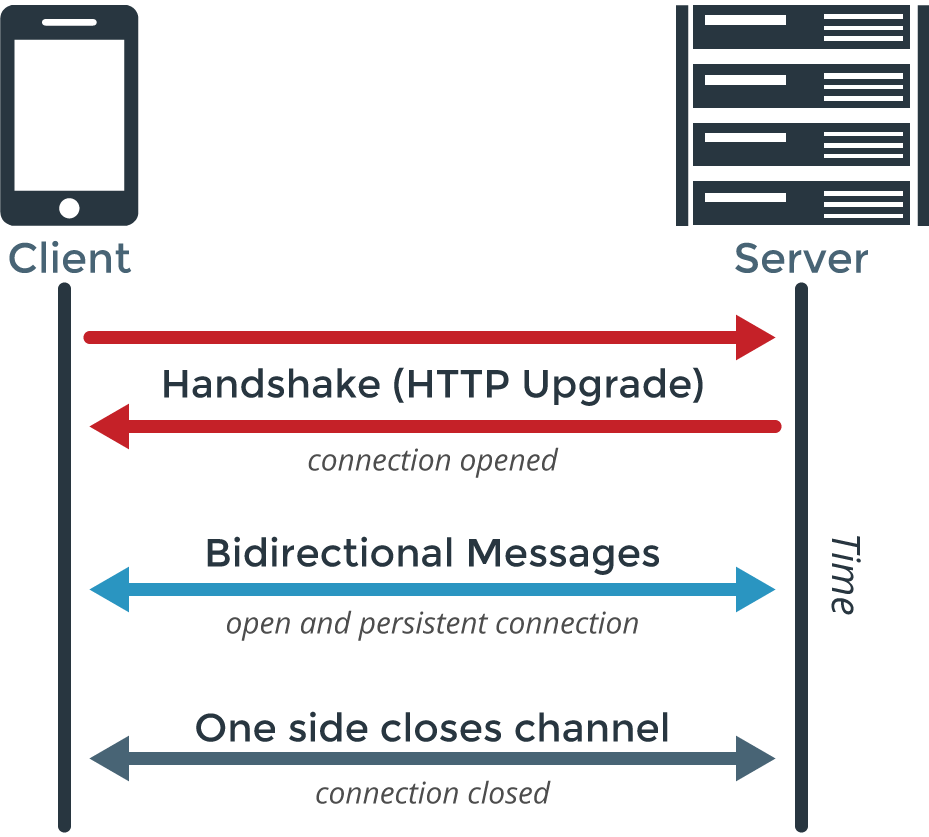
\includegraphics[scale=0.3]{ws}
\caption{WebSocket Protocol}
\end{figure}

Typically mentioned benefits of using WebSocket protocol include reduced overhead in comparison with HTTP communication. After the initial handshake, only application-specific data travels between client server, as opposed to HTTP where every request/response contains headers, cookies, content type, content length, user-agent, server id, date, last-modified etc.

WebSocket protocol has an another advantage over HTTP on a TCP protocol level (on which both are based) - TCP connection only needs to be opened once per WebSocket communication, whereas for HTTP it is opened for every request (which introduces overhead).

What is more, HTTP servers are often configured to persist in a log form the start and completion of every HTTP request. This entails additional CPU cycles and costly I/O operations. Unless an application is configured to log its proprietary data, this additional logging cost is much smaller in case of WebSockets (since there is only one initial request).

Configuring a server for high-scalability WebSocket communication is no easy task, as I have learned the hard way during this research. The whole process is described in details in a dedicated section \ref{Kernel tuning}.

\subsection{Usage and Origins}\label{Client-Server Communication Improvements}

Multi-player on-line games and real-time applications with a lot of user generated content are types of application that benefit most from popularization of the WebSocket protocol.

One of the biggest advantages of WebSockets is that the server can easily send unsolicited messages to the client, rather than simply respond to client's requests (as is the case with HTTP protocol). Before WebSockets, other solutions were being developed to enable bi-directional client-server communication, yet none of them has gained such popularity and is considered as elegant.

Before WebSockets, the applications mentioned above had to resort to other, less efficient ways to facilitate bi-directional client-server communication.

% M. Franklin and S. Zdonik provide an insight into the history of push-based technologies. Their paper from 1998 [MMPROJ12] classifies communication mechanisms into aperiodic pull, periodic pull, aperiodic push and periodic push.
Agarwal presents us with an overview of protocols previously used for the same kind of communication \cite{PushScale}:
\begin{description}
  \item[AJAX]
  - asynchronous JavaScript and XML, a request/response model; when originally introduced, it was a huge improvement, since the page did not have to be refreshed anymore to get new data. Still used widely, but for a slightly different purpose than the WebSocket Protocol.
  \item[Long Polling]
  - consists of the client sending a single request and the server waits until it can provide the response (or times out), which does not create much traffic but uses a lot of server resources. Connections are artificially kept open and clients need to reconnect periodically.
  \item[Short Polling]
  - also called AJAX-based timer, consists of the client repeatedly (timer is used to regulate that) sending the same request to the server (polling), which creates a lot of useless traffic.
  \item[webRTC]
  - Web Real-Time Communication, enables audio, video and text communication between users using web browsers \footnote{\url{http://www.webrtc.org/}}.
  \item[Server-Sent Events]
  - a stream of events generated by the server, to which a client subscribes. Communication is impossible in the other direction\footnote{\url{https://developer.mozilla.org/en-US/docs/Server-sent_events/Using_server-sent_events}}.
\end{description}
%%%%%%%%%%%%%%%%%%%%%%%%%%%%%%%%%%%%%%%%%%%%%%%%%%%%%%%%%%%%%%%%%%%%%%%%%%%%%%%%

%%%%%%%%%%%%%%%%%%%%%%%%%%%%%%%%%%%%%%%%%%%%%%%%%%%%%%%%%%%%%%%%%%%%%%%%%%%%%%%%
\chapter{Benchmarking}\label{Benchmarking}

\epigraph{"If you're not keeping score, you're just practicing."}{--- Vince Lombardi, American Football Player}

As this projects concerns benchmarking different architecture decompositions of The System Under Test \ref{The System Under Test}, it is important to define and describe the benchmarking process.

\begin{description}
  \item[Benchmarking]
  - the term is most commonly defined as an execution of a set of operations against a given object / program, in order to determine it's relative performance. Usually, it consists of a set of standardized tests. The same term is often used to describe benchmarking programs themselves. It is crucial for researchers, tool developers and users \cite{BenRM}.
\end{description}

As James Bornholt describes in his article \cite{BornBen}, computer science research is among the most non-deterministic. A huge risk of omitted-variable bias exists. This is due to the fact that computer systems have a tremendous number of dynamic parts (both in hardware and software). It is virtually impossible for researches and other experts to have complete knowledge of every bit of the system they are working with. Controlling all the involved variables is insurmountable.

Furthermore, many of the system parts factors are non-deterministic; e.g. networks and multi-threading. Because of that, researchers need to be very careful when attempting to draw statistically meaningful conclusions from their research.

Benchmarking a distributed system is even more complex \cite{BornBen}. If it is hosted in a cloud environment, the control over the hardware is in the hands of the cloud provider, not the researcher. This is situation I am in performing this research.

Bornholt \cite{BornBen} lists some of the many environmental factors that can have influence on the performance of a computer system. The most striking example is the \textit{linking order}, which can significantly bias the results of a benchmark. As UNIX systems are highly customizable, it is important to keep the values of environmental variables as consistent as possible across benchmarking sessions.

Author also states a need for the scientific community to unify and standardize the tools for benchmarking systems. A lot of researchers rebuild their infrastructures and build their scripts anew on every project. This is where I hope to contribute to the scientific and open source communities with releasing all the possible parts of the tooling build for the purpose of this project (described in details later \ref{Experiment deliverables}).

For a benchmark to be dependable, results need to be reproducible \cite{BornBen}. That means the same results can be obtained reruning the benchmark later on a machine with the same hardware and the same software versions. Reproducibility of experimental results requires measurements to be reliable. A measurement can be called reliable, if the method guarantees accuracy (small systematic and random measurement error, i.e., no bias or "volatile" effects, resp.) and sufficient precision.

Beyer et al \cite{BenRM} list well-established benchmarks for specific tasks:
\begin{description}
  \item[SPECi]
  - The Standard Performance Evaluation Corporation\footnote{\url{https://www.spec.org/}}. They provide benchmarks for CPUs, Graphic Cards, Java Client/Servers, Mail Servers and others.
  \item[TPC]
  - Transaction Processing Performance Council\footnote{\url{http://www.tpc.org/}}. They provide benchmarks for Transaction Processing (OLTP), Decision Support, Virtualization and Big Data.
  \item[nlrpBENCH]
  - Natural Language Requirements Processing\footnote{\url{http://nlrp.ipd.kit.edu/}}. They provide benchmarks for Requirements Engineering.
\end{description}

In case of the system being benchmarked in this research \ref{The System Under Test}, it is hard to reuse any of these since the performance depends on a custom set of operations spreading across multiple system layers.

Authors of "Benchmarking cloud serving systems with YCSB" \cite{Ycsb} point out that it is important to have random distributions for benchmarking loads - \textit{uniform}, \textit{zipfian}, \textit{latest}, \textit{multinomial}, etc.

From my own experience, I have drawn that against a complex system like our utilizing a wide stack of technologies, benchmarking tool should do a few "dry runs" in order to give caches a chance to fill up, internal tables to get populated or cloud components to be warmed up (e.g. Elastic Load Balancers in case of our stack \ref{Cloud architecture setup}).

One also has to be aware of what the potential congestions are. For instance, without properly tuning the operating system's TCP stack, one has to wait a few minutes between load testing runs to let all the TCP sockets return to a usable state (that is exit the TIME\_WAIT state, unless the operating system is tuned to reuse such sockets). Details of the process of tuning are describe in detail later \ref{Kernel tuning}. In the process of testing, I have also realized our API Server takes a substantial amount of time to handle disconnects by huge number of clients (test suite disconnects all of them at the same time). That means there needs to be a non-zero pause between load test suite reruns.

\section{Benchmarking Crimes}

Gernot Heiser prepared a list \cite{GerHeiBench} of \textit{benchmarking crimes} which should be avoided when attempting to benchmark a system.

\subsubsection{Selective benchmarking}
\begin{enumerate}
  \item Not covering the full evaluation space.
  \item Not evaluating potential performance degradation.
    \begin{enumerate}
      \item \texttt{Progressive Criterion} - performance actually does improve significantly in area of interest.
      \item \texttt{Conservative Criterion} - performance does not significantly degrade elsewhere.
    \end{enumerate}
    For a benchmark to be reliable, both criteria need to be demonstrated. I trust the models that have been selected to reason about system properties \ref{Selected Meters and Metrics} are living up that task.

    As an economist Mielton Friedman used to put it, \textit{there's no such thing as free lunch}\footnote{\url{http://www.amazon.com/Theres-Such-Thing-Free-Lunch/dp/087548297X}}.

    In this context, we can interpret it in the following way. Techniques improving performance in some capacity usually entail an additional cost (extra bookkeeping, caching). As Heiser writes: "This is really at the heart of systems: it's all about picking the right trade-offs" \cite{GerHeiBench}. In our case the potential improved performance comes at a cost of increased data transfers between data centers (and therefore costs) and simply increased complexity of certain system layers.
  \item Subsetting a benchmark without strong justification. A warning sign that one might sin in this way:
    \begin{itemize}
      \item "we picked a representative subset", "typical results are shown" - reads as "we cherry picked the data to fit our expected results".
    \end{itemize}
    If benchmarking is performed on a subset of a system, a strong justification needs to be as to why a given subset of functionalities / components was selected. I am benchmarking a real-life system use case.
  \item Selective data set hiding deficiencies. Luckily, more and more statistical tools are being developed to detect that \footnote{\url{http://dataskeptic.com/epnotes/ep55_detecting-cheating-in-chess.php}}.
\end{enumerate}

\subsubsection{Using the same dataset for calibration and validation}
The way to avoid this is to calibrate the system first (using calibration workload). Then, one should use evaluation workload to show how accurate the model is. Both workloads need to be disjoint.

\subsubsection{Providing o indication of significance of data}
An example of this fallacy would be providing raw averages, without any indication of variance. At least standard deviations must be quoted. If in doubt, Heiser recommends using student's t-test to check significance \cite{GerHeiBench}.

\subsubsection{Benchmarking of simplified simulated system}
I am performing the tests on the full system deployed in the exact same environment as the production system.

\subsubsection{Using inappropriate and misleading benchmarks}
The tests are being performed on different versions of the proprietary system. The business goal of the host organization of the research is to find the best architecture - the benchmarking process is supposed to help with this. There is no incentive to be dishonest.

\subsubsection{Unfair benchmarking of competitors}
The aforementioned applies.

\subsubsection{Providing relative numbers only}
Heiser suggests this reads as "I am covering that the results are really bad or irrelevant" \cite{GerHeiBench}. In the case of this research, some results need to stary relative since this is what the selected scalability measurement meters \ref{Selected Meters and Metrics} require. Absolutes might not make sense in this context.

\subsubsection{Providing no proper baseline}
Often the state-of-the-art solution can be used as a baseline. I believe the solution we picked as a baseline (the simplest architecture decomposition) is a good one. The research leading up to the test did not yield any data to prove that statement wrong.

\subsubsection{Using arithmetic mean for averaging across benchmark scores}
Wallace and Fleming \cite{Fleming} point out that this is an incorrect way to approaching averaging.
The proper way to do this (i.e. arrive at a single figure of merit) is to use the \textit{geometric mean of the normalized scores.}

%%%%%%%%%%%%%%%%%%%%%%%%%%%%%%%%%%%%%%%%%%%%%%%%%%%%%%%%%%%%%%%%%%%%%%%%%%%%%%%%

%%%%%%%%%%%%%%%%%%%%%%%%%%%%%%%%%%%%%%%%%%%%%%%%%%%%%%%%%%%%%%%%%%%%%%%%%%%%%%%%
\chapter{The System Under Test}\label{The System Under Test}

A system under test can be best described as a \textit{real-time, dynamic, parimutuel prediction market}. It is a platform with a publicly exposed RESTful and WebSocket APIs \footnote{\url{http://instamrkt.github.io/slate/}}, through which system clients can connect their websites and mobile applications to access functionality. The scope of this project concerns the WebSocket API.

The core functionality of the platform is to allow users to make predictions on (near) future events. Users can also ask their own questions regarding these events and send them out globally or to their friends. The events can literally be anything - users' imagination is the limit. A simple use case of the system would be a live football match or an e-game match broadcast on a streaming service like \textit{twitch.tv\footnote{\url{http://www.twitch.tv/}}}. Questions can also be automatically generated based on an incoming stream of events regarding the e-game/sports match. The stream can consist of an "admin" inputting the events manually through the system's admin interface, or, if a game/match has an automatic stream of data available, it can also be connected to the platform.

What is important for this research, is that questions (and predictions users make on them) are organized as parimutuel pools. That means that every prediction in the pool affects the future distribution of winnings. Pennock describes it in details in his work on dynamic parimutuel markets \cite{Pari}.

In order to keep the users informed on what the current distribution is (and thus what are the multipliers for each of the available options), the updated distribution needs to be broadcast as quickly as possible to all interested users (and reach them around the same time). In a sense, every user is therefore both a consumer and a producer of data. In case when users are globally distributed this provides a set of data-distribution and latency related challenges on which I focus in this research.

\section{Sample Use Case}

As mentioned above, one of the simplest use cases of the platform is a live football match. A client, who has connected his application to the platform can now offer users real time questions and placing predictions on them.

A case illustrating the need for the research well would be \textit{UEFA Champions League}\footnote{\url{http://www.uefa.com/uefachampionsleague/}} final, for instance between \textit{Real Madrid} and \textit{FC Barcelona}. These events generate viewership in the range of hundreds of millions \footnote{\url{http://www.uefa.com/uefachampionsleague/news/newsid=2111684.html}}.

Let's assume we have 10 million users connected to the platform throughout the game. Most of them come from Spain and the rest of Europe (65\%). Since the time-zone suits football-loving South Americans well, a lot of users are connected from there too (20\%). The platform also hosts some North American fans (5\%), with the rest comprised of hard-core Asian (9\%) and Australian (1\%) fans.

The company providing a real-time data feed for the game have their servers located in a UK-based data center.

This raises a few interesting questions that are explored within this research:

\begin{enumerate}
  \item Where should WebSocket server instances, which distribute messages, be spun up for minimal user-platform latencies and optimal general system performance?\footnote{Optimal as defined in the Scalability Measurements chapter \ref{Scalability Measurements}.}
  \item How big should the instances be?
  \item What should be the geographic distribution of the instances? How should users be routed to them?
  \item What should be the data-layer architecture? Should the data be centralized or distributed? Distributing using replication, sharding, or some other clustering technique?
\end{enumerate}

\section{Users of the System}

The users have a possibility to connect to the platform from any mobile and desktop device that supports WebSocket communication protocol. That means they can use the platform during live games in stadiums (more and more of which provide good network connectivity), watching sports on TV or e-gaming streams from their couch or in bars and other gatherings with their friends.

That means the platform has to be capable of working efficiently not only on cable and strong wi-fi networks, but also on 4g and 3g networks to facilitate mobile usage. As the experts at AT\&T inform\footnote{\url{http://developer.att.com/application-resource-optimizer/docs/best-practices/multiple-simultaneous-TCP-connections}}, latency is more of an issue or wireless networks than on wired ones. This is because wireless network is more constrained in size and scope than a wired one. The wireless connections there need to be managed more carefully. Most usage is expected to come from mobile networks (which often drop), so reconnecting them quick to the right instance is of huge importance.

Due to the nature of the platform, the demand is extremely lumpy and comes in a few-hour-long spikes for the big events.

\section{Basic Architecture}

The most basic architecture, in its non-distributed form, of the main WebSocket API system components is depicted on the figure \ref{figure:architecture}.

The system consists of the following units:
\begin{description}
  \item[Event Server]
  - receives and processes the external game/match related stream of events. Notifies the WebSocket API server so that it can broadcast the updates to the users.
  \item[Resolver]
  - upon an arrival of a new event, collects all the outstanding pools related to it, resolves accordingly, calculates winnings, updates accounts. Notifies the WebSocket API server so that it can broadcast the updates to the users.
  \item[WebSocket API Server]
  - handles all end-user communication. Receives requests, sends out response and broadcasts game, prediction pool and all other updates. User's subscribe to game-specific channels in order to receive updates.
\end{description}

\begin{figure}[h]
\centering
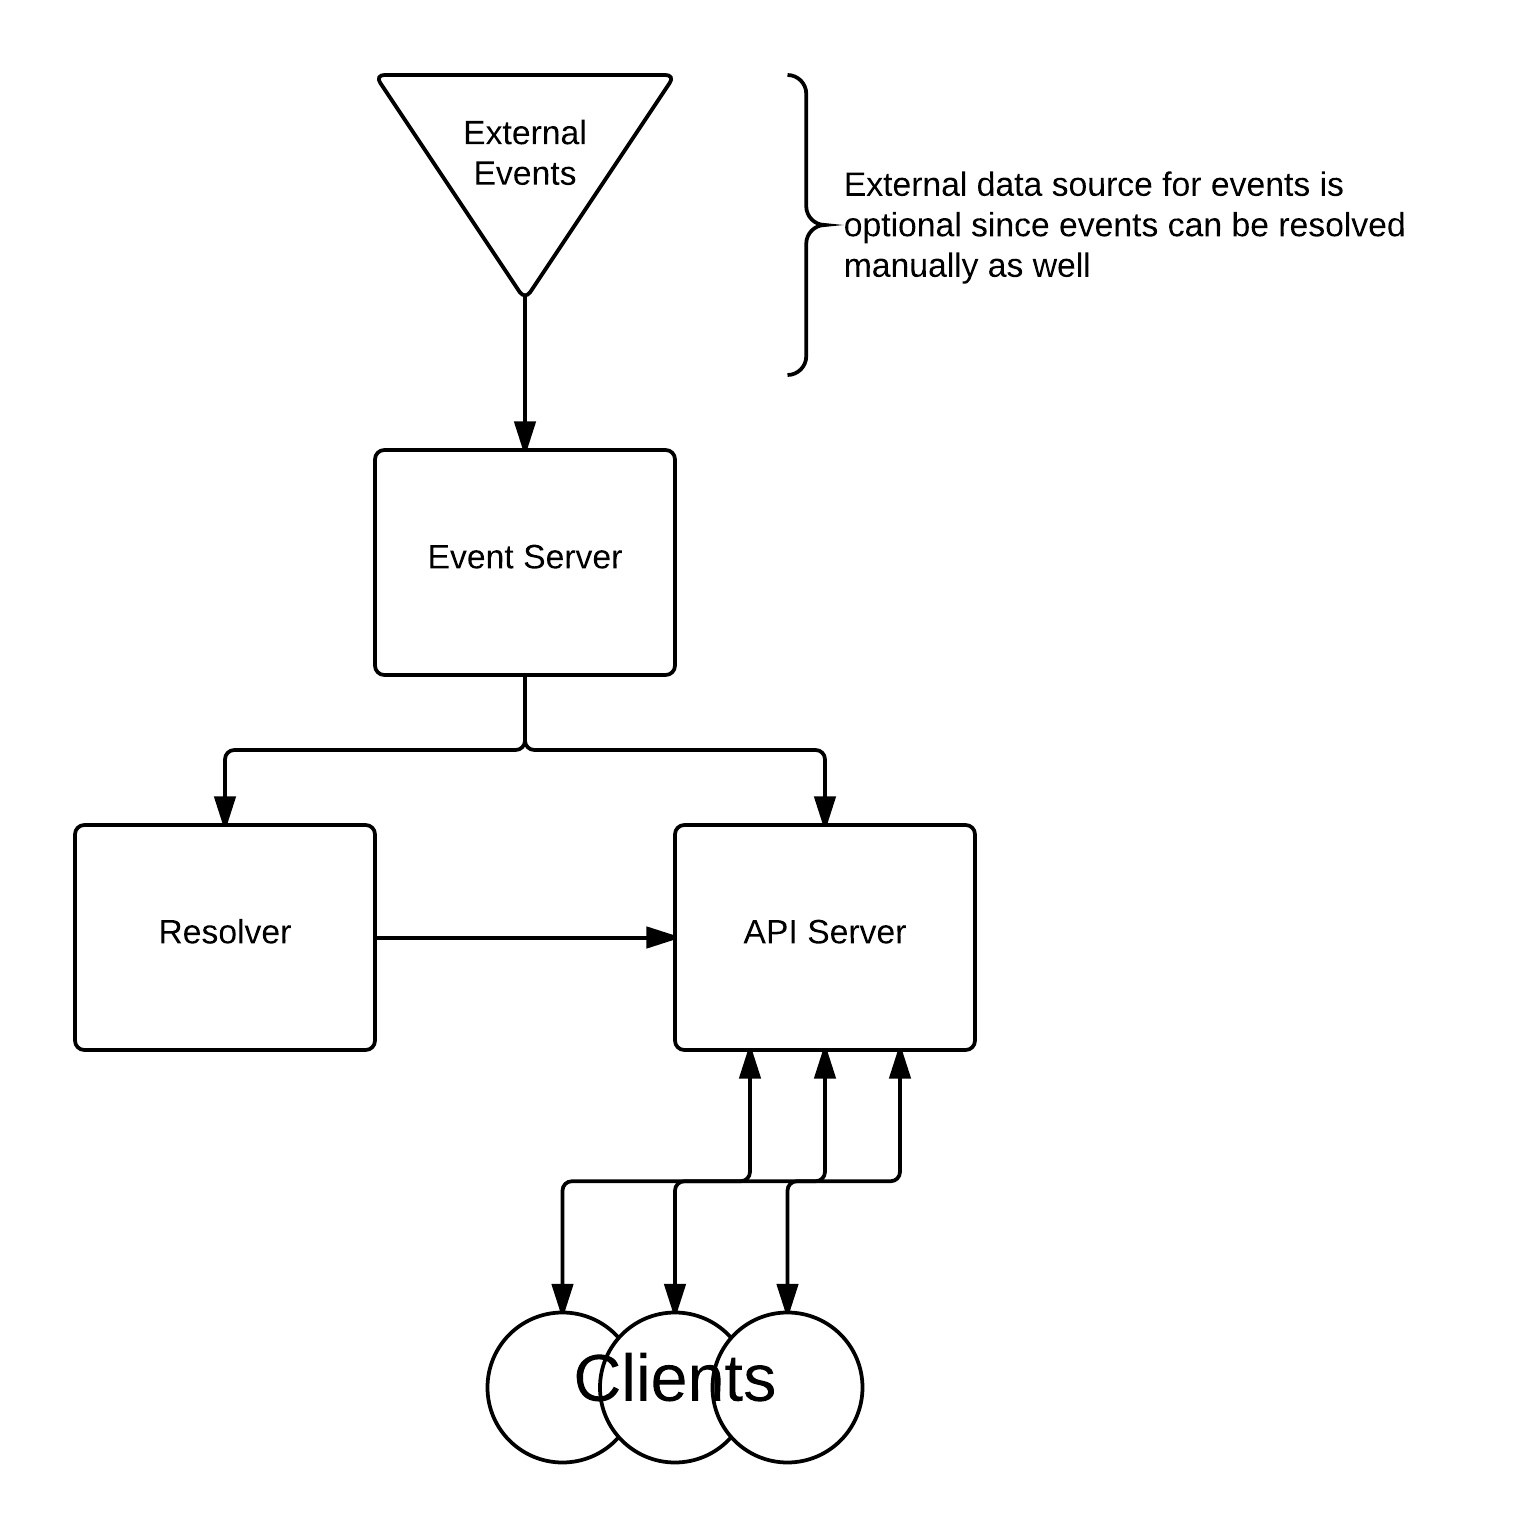
\includegraphics[scale=0.15]{architecture}
\caption{Basic System Architecture}
\label{figure:architecture}
\end{figure}

\section{Technology Stack} \label{Technology Stack}

The platform is written mostly in Python \texttt{2.7.6}. Data storages used by the platform consist of Redis \texttt{2.8.10} as a caching solution and MySQL \texttt{2.8.6} as persistent storage. A sample client application is written in Ampersand.js\footnote{\url{http://ampersandjs.com/}}. Cloud stack used to which the application is deployed is fully described later \ref{Cloud architecture setup}.

\section{Web Server}

We use nginx\footnote{\url{http://nginx.org/}} as a web server solution, which handles encrypted communication and forwards the traffic to the backend servers. If there are multiple backend servers deployed on a single machine, nginx handles the load balancing between them (using a simple round-robin routing policy).

% \subsection{Database Technologies}

% \subsubsection{MySQL Cluster}
% write scalable, important for us, multi master, automatic / manual sharding
% distributed, shared-nothing data that provides very high, scalable performance for applications that largely use primary key access and have high concurrency, but it incurs a cost in network access when accessing data between a MySQL Server and tables distributed across Data Nodes
% In terms of CAP, MySQL Cluster will sacrifice availability to maintain consistency in the event of an unsurvivable network partition.
% at least 3 machines (otherwise split brain problem)
% data nodes (ndbd) - need memory, single-threaded
% sql nodes (MySQLd) - need CPU, multithreaded
% Important:
% Will MySQL Cluster “out of the box” run an application faster than my existing MySQL database?
% The reality is probably not without some optimizations to the application and the database. However, by following the guidelines and best practices in the Guide to Optimizing Performance of the MySQL Cluster Database1 , significant performance gains can be realized, especially as you start to scale write operations while maintaining very high levels of availability and low latency.
% [http://openquery.com.au/files/MySQL-cluster-intro-use.pdf]

\section{Message Handling and Message Publishing}

The API server serves two main purposes: handling and responding to user requests, and broadcasting messages with state updates that these requests (and the system internally) generates.

These two functionalities is what my load testing focuses on. Request handling simply happens on a WebSocket protocol level, whereas publishing is done using Redis' pub-sub functionality. Users subscribe to different games - the pub-sub channels. Every channel has a listening thread, that picks up on the message and distributes it to clients connected over WebSockets.

\section{Unique Aspects of The System}

There are multiple unique aspects of the system that make this research interesting:

\begin{itemize}
  \item Critical data is communicated using the WebSocket protocol.
  \item Users receiving data shared locally should receive it at the same time as data shared globally (with as small a latency as possible). This creates a need for globally consistent and manageable latency between end user and the system.
  \item Connected users (who serve both as consumers and producers of data) and sources of data are geographically changing. Users geographical center of mass is changing for each peak of demand.
  \item Demand is extremely lumpy. This creates a need for being able to quickly the system up and down.
  \item New data is generated constantly by the users so caching the content for geographical distribution is difficult.
\end{itemize}

%%%%%%%%%%%%%%%%%%%%%%%%%%%%%%%%%%%%%%%%%%%%%%%%%%%%%%%%%%%%%%%%%%%%%%%%%%%%%%%%

%%%%%%%%%%%%%%%%%%%%%%%%%%%%%%%%%%%%%%%%%%%%%%%%%%%%%%%%%%%%%%%%%%%%%%%%%%%%%%%%
\chapter{Experiment Outline and Design} \label{Experiment Outline and Design}

\section{Goal of the experiment}

The goal of the project is to design a scalability framework for a real-time persistent WebSocket distributed application (the system). The core researched topic is whether a systems awareness of clients geographical distribution can improve the system performance according to selected metrics, in comparison with traditional approach \ref{Baseline Architecture}.

The goal of the project is to see if the proposed architecture decompositions \ref{Proposed Architecture I}, \ref{Proposed Architecture II} can perform better (quantitatively, according to the selected meters) than the baseline architecture in serving geographically dispersed clients. Approaches used to scale simple HTTP applications cannot always be translated to WebSocket applications since the communication protocol differs. WebSockets put a different kind of strain on the server machines since these need to keep the connection opened on a port for a prolonged period of time rather than simply open, server and close (as is the case with HTTP). Along the way, an answer needs to be found what level of decoupling provides best performance on each layer of a stateless persistent system. One of the properties of a system of that kind is that key value stores come under heavy load since this is where the state resides. A good solution for distributing (sharding / replicating) these also needs to be found. Same goes for persistent storage.

\section{Problem To Be Solved}
The host company is facing the problem of scaling up their system. It has been designed in a way that should support scalability - all processes are decoupled and communicate over TCP sockets, using the ZMQ library\footnote{\url{http://zeromq.org/}}. Most internal messaging happens using pub-sub architecture. Thanks to that, new nodes can be added to the system in order to increase its capacity.

Even though the system has been designed for scalability, it has note been battle-tested. The scalability process is performed in this research; multiple system limitations and have been identified \ref{Discovered System Limitations} and solutions proposed and implemented.

Our (the host company) preliminary research has not yielded definitive answers as two which level of geographic architecture decomposition will result in best system performance. The key metrics influencing these performance are user-experienced WebSocket handshaking, message handling latencies, utilization of the allocated cloud resources and utilization cost.

Furthermore, the organization does not possess any tools to measure application performance. This research provides the organization with a set of tools to measure any component of the system (in terms of resource usage and processing time), store the metrics and visualize them in real-time in a comprehensible way.

On top that, my research delivers the design and implementation of the load testing suite, including cloud client operating system images, orchestration scripts for simulating the load testing from the clients and collecting the metrics onto a master machine.

\section{Question to be answered}
\begin{enumerate}
  \item What's the architecture decomposition stack that:
    \begin{enumerate}
      \item guarantees data delivery to geographically distributed users with minimal, consistent and manageable latency?
      \item guarantees lowest cost and best degree of utilization of the employed resources within a data center?
    \end{enumerate}
  \item Does architecture with geographical awareness of its users' distribution provide better Quality of Service than the baseline architecture?
\end{enumerate}

The answer to these questions is sought for among the 3 tested architecture, described in detail below \ref{Compared Architectures}. In short - I propose 3 architectures of increasing level of geographical distribution (= decreasing level of centralization) and then use the load test and measurements suite to assess which performs best.

Answers to these questions are evaluated using the models and a set of metrics described in detail in a dedicated chapter \ref{Scalability Measurements}, section \ref{Selected Meters and Metrics}.

\section{Research Method}
The research method I selected is \textit{Controlled experiment} \ref{Research Method}. The \textit{controlled} part is somewhat tricky in the cloud environment. The intrinsic property of cloud computing is that the researcher has to give up control over hardware to the cloud provider, thus fully controlling it cannot be in scope of a project such as mine. Nevertheless, I did my best to keep constant all variables I have influence over and measure and control all the rest.

Variables constant across benchmark runs against different architectures include:
\begin{itemize}
  \item Number of connecting users (24,000),
  \item Pace at which users connect (120 users per second),
  \item Number of requests that need to be handled (with some random, controlled variance),
  \item Number of updates that need to be broadcast (with some random, controlled variance),
  \item The length of the benchmark execution,
  \item Selected instance types (with controlled variance, different decompositions require different components)
\end{itemize}

Variables over which I have no full control:
\begin{itemize}
  \item allocated network bandwidth for cloud instances,
  \item spikes in resource allocation on shared cloud instances (e.g. Allocated CPU cycles) (this happens mostly for micro instances \footnote{\url{http://docs.aws.amazon.com/AWSEC2/latest/UserGuide/concepts\_micro\_instances.html}}, I use bigger instances),
  \item general global network conditions (benchmarks are run at the same time of a day, at times [to my best knowledge] with no major global events which could disrupt network conditions).
\end{itemize}

\section{Experiment Outline}

In this section I list all the steps necessary for the experiment to be prepared and executed.

\subsection{Pre-experiment preparations}

This consists of two main parts: preparing the load test suite and the deployed system.

\subsubsection{Load Test Suite}

The following steps are necessary to deploy the load test suite:
\begin{enumerate}
  \item copy the load test client instance image to all AWS regions,
  \item for each region, start the desired number of instances using the image.
\end{enumerate}

\subsubsection{The System}

This varies slightly depending on the deployed architecture; below I list the general outline:
\begin{enumerate}
  \item prepare the clean server (and database if necessary) instance image and distribute it across relevant regions (clean means no unnecessary data stored and no redundant services running),
  \item start the instances,
  \item clean redis and MySQL and populate with data necessary for the benchmark run,
\end{enumerate}

Once all the client and server instances are brought up and reachable (verifiable through AWS API), the load test can begin.

\subsection{Load Testing}\label{Load Testing}

Simulated clients come from instances located in all available Auto-Scaling AWS regions \footnote{\url{http://docs.aws.amazon.com/general/latest/gr/rande.html}}, except for eu-central-1 (Frankfurt) \ref{Exluding Frankfurt Region}.

The load testing process is enumerated below:
\begin{enumerate}
  \item The single master node orchestrating the suite collects IP addresses of the client instances,
  \item it connects to all the client instances (using a library utilizing ssh) and issues a \textit{start test} command,
  \item it sleeps for a specified amount of time,
  \item it connects to clients again and kills the client processes,
  \item it sleeps for a small amount of time to let client processes close all connections, process collected metrics and save them to a temporary file,
  \item it connects to clients again and copies the file to master node where metrics are aggregated.
\end{enumerate}

\subsection{Users Distribution}\label{Users Distribution}

Since this is going to differ for a type of game served on the platform, I decided to use the most basic distribution - the same number of users connecting from each of the 8 available regions: North Virginia, Oregon, North California, Ireland, Singapore, Sydney, Tokyo and Sao Paulo.

\subsection{Used Benchmarking Scenario}\label{Used Benchmarking Scenario}

The benchmarking scenario is the same for each tested architecture. As mentioned before, clients connect from 8 globally-distributed regions, 15 instances in each region, each with the same number of clients. Each instance connects one client a second, so in total $8*15=120$ are connected every second until the full load is reached. The full load has been set at \texttt{24000} users, so each instance connects 200 users.

Once all the users have connected, the benchmark runs for exactly 90 minutes and then all the clients disconnect.

Upon connecting, each users lists available games (which there is one during the benchmark run), \textit{thinks} between 0 and 15 seconds, joins a game (to subscribe to all game updates) and lists available prediction pools for the game (which there is also only one for the benchmark run). Once this is completed, each users places a prediction every (0,30) seconds (once the prediction confirmation is received, the counter is reset). This continues until the benchmark run is finished.

The server responds to each user request and sends out an unsolicited pool distribution update every 3 seconds.

\begin{sourcecode}
\begin{lstlisting}[language=javascript]
var _ = require('underscore');

// max delays in milliseconds
var MAX_GAME_SELECTION_DELAY     = 15000;
var MAX_PREDICTION_PLACING_DELAY = 30000;

// called upon reception of the list of active games by the client
var handleActiveGames = function(msg) {
  // ... handle reception of list of active games

  // simulate user thinking and selection of a game
  setTimeout(function() {
    game = selectGame();
    listAvailablePoolsForGame(game.game_id);
    subscribeToGame(game.game_id);
  }, _.random(1000, MAX_GAME_SELECTION_DELAY));
};

// called upon reception of the list of active pools for game by the client
// and upon confirmation of prediction placing
var handlePoolsList = function(msg) {
  // ... handle reception of list of active pools

  // simulate user thinking and placing prediction
  setTimeout(function() {
    pool = selectPool();
    placePredictionInPool(pool);
  }, _.random(1000, MAX_PREDICTION_PLACING_DELAY))
};

\end{lstlisting}
\caption{Code simulating users joining games and placing predictions.}
\end{sourcecode}

\subsubsection{Why is this benchmark representative?}

It's the expected load during a football (soccer) game. The load is \textit{expected}, since the system has not been run at this scale yet - that's partly why the host company is in need of a project like this one.

User's load is representative of that scenario - users connect over a few minutes before the game starts, then stay connected over 90 minute game load and then disconnect once the game is finished.

\section{Compared Architectures}\label{Compared Architectures}

This section contains simple descriptions and diagram overviews of the compared architectures. Implementation details can be found in the following chapter \ref{Compared Architectures Implementation Details}.

\subsection{Baseline Architecture}\label{Baseline Architecture}
The baseline architecture consists of the main three components (the WebSocket server, redis and MySQL) on one massive EC2 instance located in the eu-west-1 AWS data center (Ireland). Clients from all regions connect directly to the WebSocket server on this EC2 instance \ref{figure:baseline}.

\begin{figure}[H]
\centering
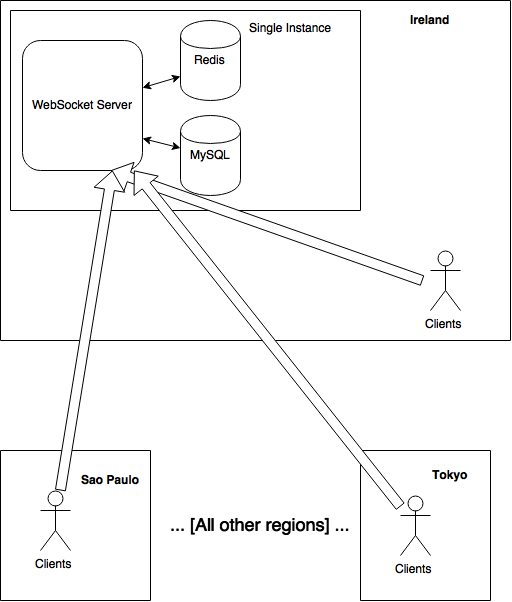
\includegraphics[scale=0.3]{baseline}
\caption{Baseline architecture diagram.}
\label{figure:baseline}
\end{figure}


The technical specification of the instances, number of processes and other technical details can be found in the next chapter \ref{Baseline Architecture Implementation Details}.

\subsection{Proposed Architecture I}\label{Proposed Architecture I}
The first proposed architecture improvement consists of the moving the WebSocket servers closer to users. This means each of the 8 regions has its own WebSocket server instance - 8 times smaller than one massive instance in case of the baseline architecture \ref{figure:archprop1}.

Database instances are still not distributed and are both located in Ireland. Clients are routed through Amazon's route53 based on their latency or geo-location.

\begin{figure}[H]
\centering
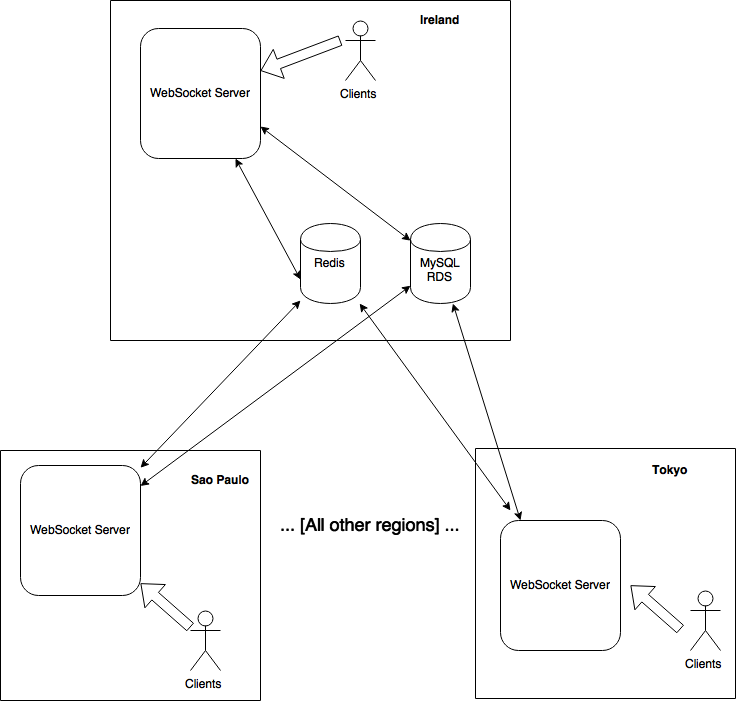
\includegraphics[scale=0.3]{archprop1}
\caption{Proposed architecture I diagram.}
\label{figure:archprop1}
\end{figure}

The technical specification of the instances, number of processes and other technical details can be found in the next chapter \ref{Proposed Architecture I Implementation Details}.

\subsection{Proposed Architecture II}\label{Proposed Architecture II}
The second proposed architecture adds the distribution of the data layer. Read replicas are placed, together with WebSocket servers, in each of the regions. Database (both MySQL and redis) writes still are routed to the master node located Ireland \ref{figure:archprop2}.

\begin{figure}[H]
\centering
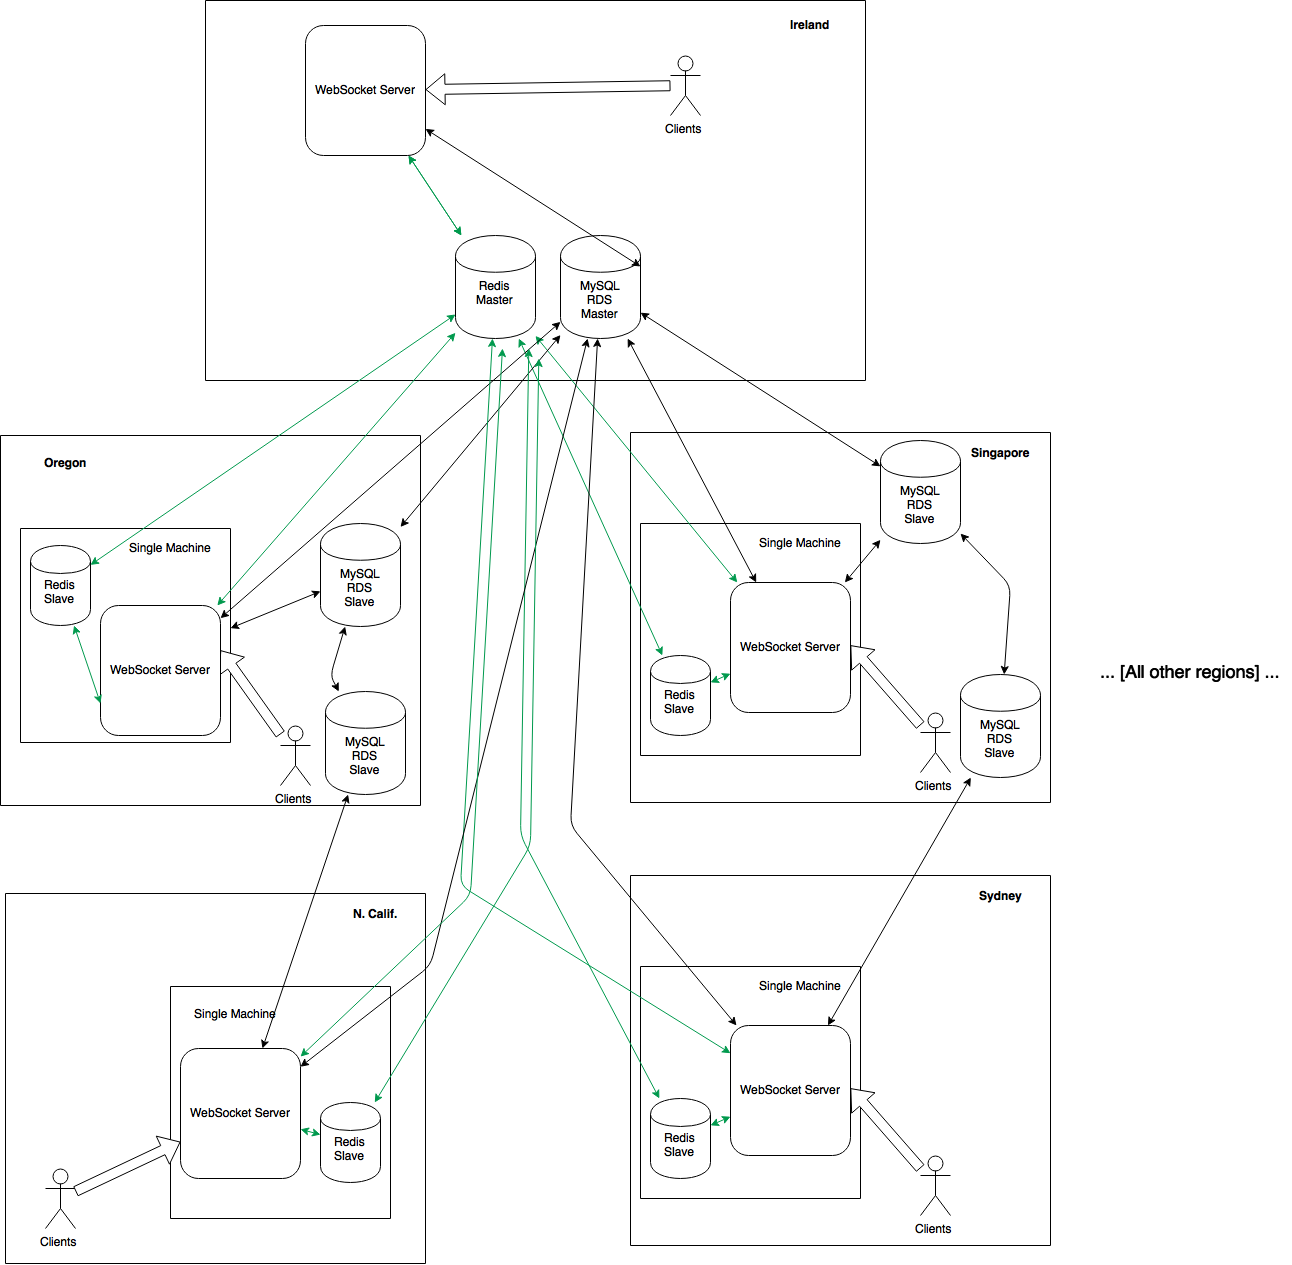
\includegraphics[scale=0.3]{archprop2}
\caption{Proposed architecture I diagram.}
\label{figure:archprop2}
\end{figure}

The technical specification of the instances, number of processes and other technical details can be found in the next chapter \ref{Proposed Architecture II Implementation Details}.

\section{Results Evaluation}
Results are evaluated using literature-based scalability meters \cite{Models}. I selected (ans slightly modified - added cost factor) the ones \ref{Selected Meters and Metrics} which best facilitate reasoning about factors most important to the host organization - client latencies, cloud resources utilization and operating cost. The tested architectures are compared using these quantifiable meters.

The selected meters allow to compare deployed architectures in general scalability terms, but also provide insight into specific aspects of the system, so that analysis can be broken down and architectures can be compared in terms of e.g. latency or cost exclusively.

\section{Experiment deliverables}\label{Experiment deliverables}

The project delivers the following:
\begin{enumerate}
  \item open sourced code for:
  \begin{itemize}
    \item using the scalability meters,
    \item managing the AWS-based region-distributed server suite (built on top of boto \footnote{\url{https://boto.readthedocs.org/en/latest/}}),
    \item remote execution of WebSocket load testing and latency-related metric collection,
  \end{itemize}
  \item a framework for comparison multiple aspects of different variants of The System Under Test \ref{The System Under Test}.
  \item a thorough analysis of the deployed architectures,
  \item improved system scalability (multiple limitations and suboptimal design decisions have been identified in the process \ref{Discovered System Limitations}).
\end{enumerate}

%%%%%%%%%%%%%%%%%%%%%%%%%%%%%%%%%%%%%%%%%%%%%%%%%%%%%%%%%%%%%%%%%%%%%%%%%%%%%%%%

%%%%%%%%%%%%%%%%%%%%%%%%%%%%%%%%%%%%%%%%%%%%%%%%%%%%%%%%%%%%%%%%%%%%%%%%%%%%%%%%
\chapter{Scalability Measurements} \label{Scalability Measurements}
In this chapter I describe most relevant models and metrics from scientific literature and the subsets I decided to use in this research \ref{Selected Meters and Metrics}.

\section{Scalability Meters}
Models I find most useful were proposed by Pattabiraman et al \cite{Models}. As mentioned in Related Work section \ref{Related Work}, they divide the performance indicators into three groups and propose formal quantifiable meters for each of them:
\begin{enumerate}
  \item computing resource indicators (CPU, disk, memory, networks, etc.),
  \begin{itemize}
    \item Computing Resource Allocation Meter (CRAM),
    \item Computing Resource Utilization Meter (CRUM),
  \end{itemize}
  \item workload indicators (connected users, throughput and latency, etc.),
  \begin{itemize}
    \item System Load Meter (SLM),
  \end{itemize}
  \item performance indicators (processing speed, system reliability, availability)
  \begin{itemize}
    \item System Performance Meter (SPM).
  \end{itemize}
\end{enumerate}
They also propose model which allow to combine the above: System Capacity Meter (SCM), System Effective Capacity Meter (SEC), Effective System Scalability (ESS), and Effective Scalable Range (ESR).

\subsection{Scalability Meters}

The geometric interpretation of each of these meters is a polygon. The quantifiable value of the meter is the area of the polygon. Sample meter is plotted on the figure \ref{figure:polygon}.

\begin{figure}[h]
\centering
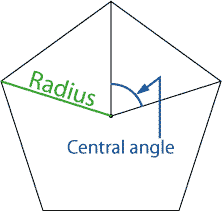
\includegraphics[scale=0.5]{angleradius}
\caption{Polygon's radius and central angle}
\label{figure:polygon1}
\end{figure}

The value of each metric plugged into the meter is represented by the radial distance between the center of the polygon and the vertex. Since all the metrics that serve as inputs to the meter have equal weights, the central angle (as shown of figure \ref{figure:polygon1}) between two consecutive radial distances is always going to be equal. For \textit{$n$} metrics in a meter, each central angle will have a value of \textit{$2\Pi/n$}.

The area of a polygon can be computed as a sum of areas of the triangles that constitute it. The sides of each of these triangles consist of the side of the polygon and 2 radii.

Area of a triangle can be computed using the formula:
\begin{center}
  $$A_t = 0.5 * a*b * \sin(\alpha_{ab}) $$
  where \textit{$a$} and \textit{$b$} are to sides of the triangle and $\alpha_{ab}$ is the angle between them.
\end{center}

In case of these meters, $\alpha_{ab}$ is always equal to $2\Pi/n$. The area of a triangle limited by two radii with values of two metrics $x_i$ and $x_{i+1}$ would look like this:
\begin{center}
  $$A_t = 0.5 * x_i*x_{i+1} * \sin(2\Pi/n) $$
\end{center}

To compute the area of the polygon one needs to sum all the areas of the triangles formed by radii, and thus the formula is the following:
\begin{center}
  \texttt{$$A_p = 0.5 * \sin(2\Pi/n) * \sum_{i=1}^{n}x_i*x_{i+1}$$}
  where \textit{$x_i$} is a value of an input metric and \textit{n} is the count of input metrics.
\end{center}

\begin{figure}[h]
\centering
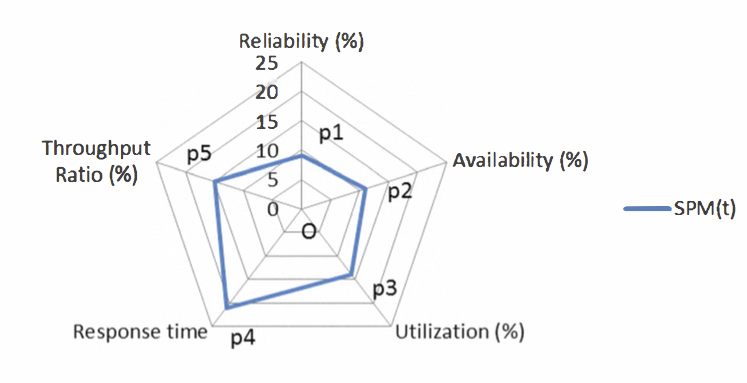
\includegraphics[scale=0.5]{polygon}
\caption{Sample Meter Geometric Interpretation (SPM)}
\label{figure:polygon}
\end{figure}

\subsubsection{Computing Resource Allocation Meter (CRAM)}
\begin{center}
  $$CRAM(S,t) = 0.5 * \sin(2\Pi/n) * \sum_{i=1}^{n}a_i*a_{i+1}$$
\end{center}
  \texttt{$S$} - represents the measured system, \\*
  \texttt{$t$} - represents the time over which total resource allocation for the system is evaluated, \\*
  \texttt{$a_i$} - represents the values of different types of \textit{allocated} computing resources to S by a cloud (network traffic boundary, cache allocated, memory allocated, CPU allocated, etc.), \\*
  \texttt{$n$} - represents the count of different types of allocated computing resources to S by a cloud.

\subsubsection{Computing Resource Utilization Meter (CRUM)}
\begin{center}
  $$CRUM(S,t) = 0.5 * \sin(2\Pi/n) * \sum_{i=1}^{n}u_i*u_{i+1}$$
\end{center}
  \texttt{$S$} - represents the measured system, \\*
  \texttt{$t$} - represents the time over which total resource allocation for the system is evaluated, \\*
  \texttt{$u_i$} - represents the values of different types of computing resources \textit{utilized} by S in a cloud (network traffic boundary, cache allocated, memory allocated, CPU allocated, etc.), \\*
  \texttt{$n$} - represents the count of different types of computing resources utilized by S in a cloud.

\subsubsection{System Performance Meter (SPM)}
\begin{center}
  $$SPM(S,t) = 0.5 * \sin(2\Pi/n) * \sum_{i=1}^{n}p_i*p_{i+1}$$
\end{center}
  \texttt{$S$} - represents the measured system, \\*
  \texttt{$t$} - represents the time over which system performance is evaluated, \\*
  \texttt{$p_i$} - represents the values of different performance metrics of the S in a cloud  (throughput ratio, reliability, availability, utilization, response time, etc.), \\*
  \texttt{$n$} - represents the count of different performance metrics measured in S.

\subsubsection{System Load Meter (SLM)}
\begin{center}
  $$SCM(S,t) = 0.5 * \sin(2\Pi/3) * [CTL(t)*UAL(t)+UAL(t)*SDL(t)+CTL(t)*CDL(t)]$$
\end{center}
  \texttt{$S$} - represents the measured system, \\*
  \texttt{$t$} - represents the time over which load for the system is evaluated, \\*
  \texttt{$CTL(t)$} - represents system communication traffic load, \\*
  \texttt{$UAL(t)$} - represents system user access load, \\*
  \texttt{$SDL(t)$} - represents system data load. \\*

\subsubsection{System Capacity Meter (SCM)}
\begin{center}
  $$SCM(S,t) = 0.5 * \sin(2\Pi/3) * [SL(t)*SP(t)+SL(t)*AR(t)+SP(t)*AR(t)]$$
\end{center}
  \texttt{$S$} - represents the measured system, \\*
  \texttt{$t$} - represents the time over which system capacity is evaluated, \\*
  \texttt{$SL(t)$} - represents system load based on SLM, \\*
  \texttt{$SP(t)$} - represents system performance based on SPM, \\*
  \texttt{$AR(t)$} - represents system resource allocation based on CRAM. \\*

\subsubsection{System Effective Capacity Meter (SEC)}
\begin{center}
  $$SEC(S,t) = 0.5 * \sin(2\Pi/3) * [SL(t)*SP(t)+SL(t)*RU(t)+SP(t)*RU(t)]$$
\end{center}
  \texttt{$S$} - represents the measured system, \\*
  \texttt{$t$} - represents the time over which load for the system is evaluated, \\*
  \texttt{$SL(t)$} - represents system load based on SLM, \\*
  \texttt{$SP(t)$} - represents system performance based on SPM, \\*
  \texttt{$RU(t)$} - represents system resource utilization based on CRUM. \\*

Since all the meters above use the values sampled over a period of time as input, for each of the mentioned meters one can talk about \textit{min} and \textit{max} values. This is useful for the last two meters.

\begin{figure}[h]
\centering
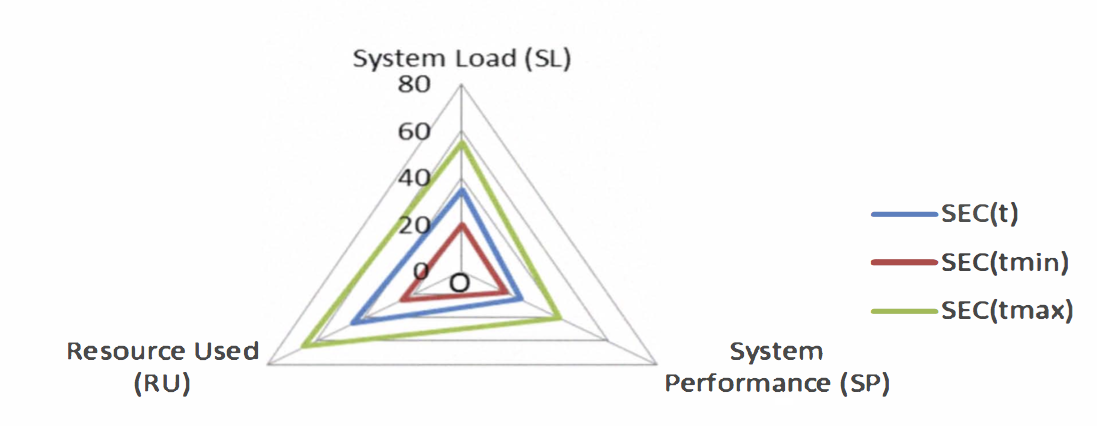
\includegraphics[scale=0.3]{sec}
\caption{Sample System Effective Capacity Meter (SEC)}
\label{figure:sec}
\end{figure}

\subsubsection{Effective System Scalability (ESS)}
\begin{center}
  $$ESS = [SL(t) / SL_{min}] / [SEC(t) / SEC_{min}]$$
\end{center}
  \texttt{$t$} - represents the time over which the system is evaluated, \\*
  \texttt{$SL(t)$} - represents system load based on SLM, \\*
  \texttt{$SEC(t)$} - represents system effective capacity based on SEC. \\*

\subsubsection{Effective Scalable Range (ESR)}
\begin{center}
  $$ESR = (SEC_{max} - SEC_{min})$$
\end{center}
  \texttt{$SEC$} - represents \textit{max} and \textit{min} system effective capacity based on SEC. \\*

Using the last two models (ESR and ESS), one can compare scalability of two systems/architectures in absolute quantifiable terms.

The meters I decided to use in this research are described below \ref{Selected Meters and Metrics}.

\subsection{Other Models}
There is much more work related to the measuring scalability of distributed systems. Srinivas and Janakiram in their work \cite{SriJan} mention similar metric evaluating scalability as a product of throughput and response time (or any value function) divided by the cost factor.

They propose a model considering scalability as a function of synchronization, consistency, availability, workload and faultload. It aims on identifying bottlenecks and hence improving the scalability. The authors also emphasize the fact of interconnectedness of synchronization, consistency and availability:
\begin{center}
  $$scalability = f(availability, synchronization, consistency ,workload, faultload)$$ \\*
\end{center}

Jogalekar and Woodside \cite{EvaScaDS} propose a strategy-based scalability metric based on productivity and cost effectiveness (a function of system's throughput and its Quality of Service). It separates evaluation of throughput or quantity of work from Quality of Service (which, according to the authors, can be any suitable expression). Productivity can be computed as follows:
\begin{center}
  $$F(k) = \lambda(k) * f(k) / C(k)$$ \\*
\end{center}
  \texttt{$F(k)$} - represents the productivity of system at scale k, \\*
  \texttt{$\lambda(k)$} - represents throughput in responses/s of the system at scale k, \\*
  \texttt{$f(k)$} - represents the average value of a responses of the system at scale k, calculated from its QoS, \\*
  \texttt{$f(k)$} - represents the running cost per second of the system at scale k. \\*

Based on that, one can compute scalability metric relating systems at two different scale factors as the ratio of their productivity figures:
\begin{center}
  $$\upsilon(k_1,k_2) = (F(k_1)/F(k_2)) $$\\*
\end{center}

\section{AWS Available metrics} \label{AWS Available metrics}

Since the System Under Test \ref{The System Under Test} is deployed to Amazon's Cloud \ref{Cloud architecture setup}, the metrics of the system need to be collected as a combination of metrics offered by Amazon's measurement service (CloudWatch\footnote{\url{https://aws.amazon.com/cloudwatch/}} and our custom collection process (described here \ref{Custom Metric Collection}).

Metrics from CloudWatch are collectible by default every 5 minutes. They offer a paid \textit{detailed mode}, with which one can collect metrics every minute. From what I have experienced, even in the detailed mode, the requested metrics show up in the CloudWatch API results with a delay as high as 2 minutes.

The CloudWatch API has its limitations - for instance, the allocation and utilization of memory for EC2 instances and processes is not available. This is something we are collecting in our custom metric collection process \ref{Custom Metric Collection}.

As Pattabhiraman et al. \cite{Models} warn, there exist additional costs which are not apparent from the start.
If one exceeds 10 metrics, 10 alarms, 1,000,000 million requests, 1000 SNS email notifications, 5GB of incoming data logs or 5GB of data archiving per month then additional costs accrue. This is included in the cost estimates.

CloudWatch Alarms \footnote{\url{http://docs.aws.amazon.com/AWSEC2/latest/UserGuide/using-cloudwatch.html}} can be configured based on these metrics. They can be applied to trigger AutoScaling actions that scale the deployed system in or out automatically.

A very important limitation for the case of this research is that data cannot be aggregated automatically across AWS regions \footnote{\url{http://docs.aws.amazon.com/AmazonCloudWatch/latest/DeveloperGuide/cloudwatch_concepts.html}}.

For each metric collected for a given time window (1 or 5 minutes), CloudWatch offers the following statistics: min, max, average, sum and sample count (count (number) of data points used for the statistical calculation).

Metrics can be aggregated over different domains - instances, AutoScaling groups, Elastic Load Balancers (all instances behind it) or availability zones. Metrics for groups of instances differ from metrics for single instances.

\subsection{Instance Specific}
The following metrics can be collected on an EC2 instance level:
\begin{itemize}
  \item CPU utilization (\% and absolute),
  \item Network in/out (in bytes),
  \item Disk read/write (number of operations and bytes),
  \item Custom user-defined metrics,
  \item Instance status checks data.
\end{itemize}

All these metrics are also available at an autoscale group level. They are automatically aggregated for all instances within a group. This is what I am using in my reporting.

\subsection{Custom Instance Metric Collection} \label{Custom Metric Collection}
A lot of tools (such as pidstat, which I used during local baseline preparations) are not available on Amazon Linux. Amazon provides perl scripts that allow to add metrics to cloudwatch, such as: disk space available, disk space used, disk space utilization, memory available, memory used, memory utilization, swap used and swap utilization. The scripts are \textit{not} officially maintained\footnote{\url{http://docs.aws.amazon.com/AWSEC2/latest/UserGuide/mon-scripts.html}}.

The scripts were setup by me in the following way. On a server image, the script is running as a cron job\footnote{\url{http://www.UNIXgeeks.org/security/newbie/UNIX/cron-1.html}} and reports the metrics to cloudwatch every minute (that is the maximum avilable frequency in cloudwatch). A \texttt{warning} for this kind of usage - the script caches the instance id by default. That means that every new server instance created from an AMI with this script would report metrics for an instance from which the image was originally created. The cache flag needs to be changed to false in the script and the scripts need to be rebuild \ref{lstlisting:perl}.

\begin{sourcecode}
\begin{lstlisting}[style=mono, language=perl]
use constant {
  DO_NOT_CACHE => 0,
  USE_CACHE => 1,
};

#
# Obtains EC2 instance id from meta data.
#
sub get_instance_id
{
  if (!$instance_id) {
    # The original script uses USE_CACHE below
    # To verify that the correct instance id is used run:
    # 'wget http://169.254.169.254/latest/meta-data/instance-id'
    # and compare against what the script reports.
    $instance_id = get_meta_data('/instance-id', DO_NOT_CACHE);
  }
  return $instance_id;
}
\end{lstlisting}
\caption{Updated fragment of Amazon's custom cloudwatch metric reporting perl script.}
\label{lstlisting:perl}
\end{sourcecode}

\subsection{Load Test Metric Collection}

Each client machine generating load in the benchmarking process collects client side metrics and generates a small report. After the benchmark run, these metrics are aggregated across all client instances.

The client script measures the following: handshaking latency, request handling latency and message publishing latency. The request handling and publishing latency are computed differently: request handling latency is measured as the difference between the clients response reception timestamp and request sending timestamp. Broadcast latency is measured as a difference between client reception timestamp and server publish timestamp included in the broadcast message header (it serves mostly the purpose of showing the difference in reception times of the same message across clients). Time synchronization between different machines is explained below \ref{Time synchronization across the system}.

A sample client report is listed in the Experiment Results chapter in a dedicated section \ref{Client Report}. General metric reporting structure is pictured on figure \ref{figure:structure}.

Tools used in client reporting are described in a dedicated section \ref{Load Testing Framework}.

\begin{figure}[H]
\centering
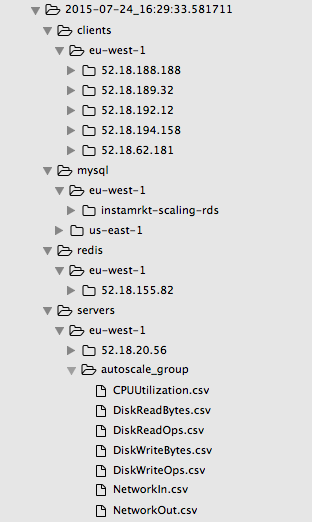
\includegraphics[scale=0.5]{structure}
\caption{Metric report structure.}
\label{figure:structure}
\end{figure}

\section{Selected Meters and Metrics}\label{Selected Meters and Metrics}
I selected the following scalability meters and metrics for their inputs:

\begin{enumerate}
  \item \texttt{Computing Resource Utilization Meter}, with inputs:
    \begin{itemize}
      \item Server CPU utilization, compiled over all server instances + redis instance and RDS instance where applicable, collected through cloudwatch,
      \item Memory utilization, compiled over all server instances + redis instance and RDS instance where applicable, collected through cloudwatch,
      \item Disk utilization, compiled over all server instances + redis instance and RDS instance where applicable, collected through cloudwatch,
    \end{itemize}
  \item \texttt{System Performance Meter}, with inputs:
    \begin{itemize}
      \item Handshaking latency, compiled over all client WebSockets on all client instances, collected through our suite,
      \item Request handling latency, compiled over all client WebSockets on all client instances, collected through our suite,
      \item Broadcast latency, compiled over all client WebSockets on all client instances, collected through our suite,
      \item Total network data in, compiled over all connections collected through cloudwatch,
      \item Total network data out, compiled over all connections collected through cloudwatch,
    \end{itemize}
  \item \texttt{System Load Meter}, with inputs:
    \begin{itemize}
      \item Successful connections, compiled over all client WebSockets on all client instances, collected through our suite,
      \item Handled requests count, compiled over all client WebSockets on all client instances, collected through our suite,
      \item Redis database successful hits, collected manually (\textit{info} command),
      \item MySQL query count, collected manually \ref{lstlisting:qcount},
    \end{itemize}
  \item \texttt{System Effective Capacity Meter}, with inputs:
    \begin{itemize}
      \item System Load Meter output,
      \item System Performance Meter output,
      \item Computing Resource Utilization Meter,
      \item Estimated cost of running a given architecture setup for a given unit of time (this is my own addition to the model from literature \cite{Models})
    \end{itemize}
  \item \texttt{Effective Scalable Scalability}, with inputs:
    \begin{itemize}
      \item System Effective Capacity Meter output,
      \item System Load Meter output,
    \end{itemize}
\end{enumerate}

\begin{sourcecode}
\begin{lstlisting}[style=mono, language=SQL]
select VARIABLE_VALUE from information_schema.global_status where variable_name = "QUERIES";
\end{lstlisting}
\caption{Extracting MySql query count.}
\label{lstlisting:qcount}
\end{sourcecode}

The benchmark is run against each of the deployed architecture setups and the resulting metrics are used to populated the described meters.

\subsection{Excluded Metrics}\label{Excluded Metrics}

I was forced to exclude some inputs I initially intended on including in the research.

\begin{description}
  \item[Availability] - I did not posses enough resources (money and time) to run the benchmark long enough to run into any availability issues, since Amazon SLAs guarantee availability of at least 99\% for the services used in this research\footnote{\url{https://aws.amazon.com/ec2/sla/}}.
  \item[Dynamic Scale Out and Scale In speed] - The way load test suite is set up is that all clients enter the system through a single url. Route53 traffic between regions according to the specified policy. Dynamically adding / removing resources causes changes to that policy - that means global DNS records need to be updated. One can set TTL (time to live), which DNS servers should respect and refresh their caches every TTL seconds. Some servers do not and this makes controlling and measuring this aspect impossible, as described in more detail later \ref{System Scaling Delay}.
\end{description}

\section{Controlling The Dynamic Cloud Environment}
It is impossible to do entirely. The number of factors that come into play is massive. Nevertheless, there are ways to have a better control over the environment. For instance, the EC2 instance types used in the research were picked so as to  be stable and have better quality guarantees (rather than unpredictable instances which offer resource spikes and collecting credits if one runs below resource under limit; that's what happens for instance on t1.micro instances). Repetitive tests were run to verify that there is no huge influential differences in allocated resources over time.

Another way to have finer control over hardware in the cloud (in AWS case) is to request dedicated rather than shared resources. It is outside of the scope of this project.

\section{Time synchronization across the system}\label{Time synchronization across the system}
The clocks on all machines are synchronized using the Network Time Protocol\footnote{\url{http://www.ntp.org/}}. All NTP daemons were synchronized with Amazon's NTP servers.

\section{Expected Answers}\label{Expected Answers}
I am going to use the \textit{Effective System Scalability} meter to perform a quantifiable comparison of the deployed architectures \ref{Compared Architectures}.

I expect to see differences in various metrics. Using all the other selected meters, I will be able to reason about specific factors of scalability (such as cost or message handling latency).

%%%%%%%%%%%%%%%%%%%%%%%%%%%%%%%%%%%%%%%%%%%%%%%%%%%%%%%%%%%%%%%%%%%%%%%%%%%%%%%%

%%%%%%%%%%%%%%%%%%%%%%%%%%%%%%%%%%%%%%%%%%%%%%%%%%%%%%%%%%%%%%%%%%%%%%%%%%%%%%%%
\chapter{Experiment Implementation} \label{Experiment Implementation}

\epigraph{"At scale, everything breaks."}{--- Urs Holzle, Google Fellow}

\section{Baseline Architecture Preparations}\label{Baseline Architecture Preparations}
In order to obtain meaningful benchmark results, I had to perform multiple optimizations of our application code. This part of the project proved extremely timely (a lot of debugging time was not budgeted for when preparing the project timeline).

I also managed to identify main resource bottlenecks. Both in cases of the client simulating process and the server, it is the CPU.

Since Node.js is single-threaded, I prepared scripts that allow to run multiple processes in parallel to utilize all cores available to the client.

As far as the WebSocket server is concerned, I have identified 2 core thread types (among many more that the server consists of) - one for request handling, another one for pushing redis-published messages through the user's WebSocket. Since TCP is a 1-1 communication protocol, a UDP-like broadcast to all WebSockets is not possible. For every channel that users subscribe to (games are channels on the domain level), the system needs a thread that listens to a redis channel and iterates over a list of WebSockets of users subscribed to that channel. These threads, and the message handling threads are by far the two most resource (CPU-bound) intensive.

This allowed us to calculate the optimal number of WebSocket server processes that should be running on each machine - the number of machine CPU cores divided by 2. Since the WebSocket servers are fully stateless, any number can be run in parallel.

\subsection{Discovered System Limitations}\label{Discovered System Limitations}

\subsubsection{Listing Pools}
The First discovered limitation was that the response with list of prediction pools for game included \textit{every} prediction made in this pool. Predictions were included so that the clients can look through them and see what predictions other users (their friends in particular) have made.

Each prediction JSON object, as depicted in snippet \ref{lstlisting:prediction}, is around 135 bytes. With a workload generated by the benchmark the number of predictions quickly goes into the thousands and tens of thousands, which already means a single message size measured in \textit{Megabytes}. This is obviously not feasible so we decided not to include all the predictions and prepare a separate request for predictions of your friends.

\begin{sourcecode}[H]
\begin{lstlisting}[style=mono,language=json]
{
    "prediction_id": "c34bcc05-58ea-4294-9310-9f8cbd121e29",
    "placed_at": 1421937458,
    "amount": 1.0,
    "user_id": 1
}
\end{lstlisting}
\caption{Single prediction JSON object.}
\label{lstlisting:prediction}
\end{sourcecode}

\subsubsection{Message Publishing}
The message publishing included in the benchmarking scenario happens when users place predictions. Each prediction influences the distribution of the pool and this information is broadcast to all users subscribed to a game to which the pool belongs.

I have discovered two huge system limitations when it comes to message publishing.

In the beginning, the distribution update was broadcast after \textit{every prediction}. For a load of 24000 users, predicting (simplifying) on average every 15 seconds, 1600 updates \textit{per second}. This is not sustainable - neither the publishing threads that had to push the message out through a list of sockets, nor the client processes could keep up with such messaging pace (or a pace nowhere near that, since publishing to a few thousand users takes hundreds of milliseconds). More importantly, humans are only capable of registering and reacting to changes as often as once every few hundred milliseconds (tested empirically \footnote{\url{http://www.humanbenchmark.com/tests/reactiontime}}). As the platform is supposed to serve as a second-screen fun, the users should not be disturbed even at that pace. Thus, we decided to batch the prediction updates and send them once every 3 seconds (per pool). This improved the performance tremendously.

At first, updating the last broadcast timestamp in redis (\textit{line 6} from the listing \ref{lstlisting:batching}) was located below line 14. When running multiple WebSocket server instances, this caused a race condition (retrieving data concerning hundreds of predictions from redis and formatting them takes up to tens of milliseconds), so up to 3 broadcast messages would be sent within a few milliseconds. This problem got solved by moving it up the if clause. The check is still not atomic, but get and set are now separated only with one integer comparison (within the if clause, \textit{line 5}, listing \ref{lstlisting:batching}) so the race condition is not expected to happen at any reasonable scale. Nevertheless, this will be made atomic eventually.

\begin{sourcecode}[h]
\begin{lstlisting}[style=mono,language=Python]
# WebSocket Handler class
# place prediction request handling

last_broadcast = db.get_pool_last_distibution_broadcast_timestamp(pool_id) or 0
if ((int(placed_at) - int(last_broadcast)) > im_configs.BATCH_FREQUENCY):
    db.set_pool_last_distibution_broadcast_timestamp(pool_id, epoch_millis())

    new_predictions = db.get_predictions_to_broadcast_for_pool(pool_id)
    distribution    = self.prepare_distributions_structure(pool_id)

    broadcast_message = im_messages.PoolDistributionUpdatedPublish(
      pool_id, new_predictions, distribution
    )
    self.do_publish(broadcast_message, game_id)
else:
  # persist for later broadcast
  db.add_prediction_ids_to_broadcast_for_pool(pool_id, prediction_id)
\end{lstlisting}
\caption{Message batching.}
\label{lstlisting:batching}
\end{sourcecode}

The second big issue was that because publishing of distribution updates was batched, every broadcast message included details of every new prediction (few hundred) made within the time window between batched broadcasts. This message would be broadcast to \texttt{every user every 3 seconds}. This was generating a tremendous, unnecessary data load. Since the purpose of this was the same as in including new predictions when listing pools, the same solution was applied. Users request their friend data separately now. Identifying this was a complete game changer - it reduced the application data load \texttt{300-fold} and allowed to increase number of sustainable users in the system by \texttt{2 orders of magnitude}.

\subsection{Kernel tuning}\label{Kernel tuning}
Operating systems are not tuned by default to sustain a huge number of concurrent users, nor are they tuned to support quick connects / disconnects and TCP sockets reusage. Because of that, I needed to dig into UNIX kernel and TCP stack handling and prepare the operating system setup on which I based the images used in the project.

Listing \ref{lstlisting:sysctl} shows all the \textit{sysctl} changes that were introduced to \texttt{/etc/sysctl.conf}. Sysctl \footnote{\url{http://linux.die.net/man/8/sysctl}} is used to modify kernel parameters at runtime. The changes are described in details below.

\begin{sourcecode}[h]
\begin{lstlisting}[style=mono]
# WebSocket scalable config
fs.file\-max = 1655360

net.core.netdev_max_backlog=65536
net.ipv4.TCP_max_syn_backlog=65536
net.core.somaxconn=16384

net.ipv4.TCP_slow_start_after_idle=0

net.ipv4.TCP_mem=383865 511820 2303190
net.ipv4.TCP_rmem=8192 873700 8388608
net.ipv4.TCP_wmem=4096 655360 8388608

net.ipv4.TCP_fin_timeout=5

net.ipv4.TCP_max_orphans=262144

net.ipv4.TCP_synack_retries=2
net.ipv4.TCP_syn_retries=2

net.ipv4.TCP_tw_reuse=1

net.ipv4.ip_local_port_range=1025 65535

vm.overcommit_memory=1
\end{lstlisting}
\caption{Sysctl.conf updates.}
\label{lstlisting:sysctl}
\end{sourcecode}

\begin{description}
  \item[fs.file-max] Maximum number of open file descriptors that can be opened by a single process. With the default value, both nginx and the WebSocket server is incapable of serving more than 1024 users.
  \item[net.core.netdev\_max\_backlog] Maximum number of packets that can be queued on interface input. If kernel is receiving packets faster than can be processed, this queue increases (high value is of this parameter is not necessary so as not to drop messages).
  \item[net.ipv4.TCP\_max\_syn\_backlog] Maximum number of remembered connection requests, which are still did not receive an acknowledgment from connecting client.
  \item[net.core.somaxconn] Max length of the listen queue backlog (processes like nginx need this value to be high for high performance). Withuot setting this value, TCP listen queue overflows happen. \textit{"possible SYN flooding on port"} in \texttt{/var/log/messages} is an indication that this value is too low.
  \item[net.ipv4.TCP\_slow\_start\_after\_idle] This value should be set to 0 to ensure connections don't go back to default TCP window size after being idle for too long.
  \item[net.ipv4.TCP\_mem] \textit{min pressure max}, Total memory pages allocated for TCP sockets. If this memory reaches pressure value, kernel starts putting pressure on TCP memory. More than \textit{max} will not be allocated. Messages \textit{"maximum number of memory pages allocated to the TCP was reached"} indicates these values are too low.
  \item[net.ipv4.TCP\_rmem] \textit{min default max}, Size of receive buffer for each TCP connection. Kernel auto tunes these values between the min-max range.
  \item[net.ipv4.TCP\_wmem] \textit{min default max}, Size of send buffer for each TCP connection. Kernel auto tunes these values between the min-max range.
  \item[net.ipv4.TCP\_fin\_timeout] Time a connection should spend in FIN\_WAIT\_2 state. By default it is set to 60s, lower values tell kernel to free memory faster and move sockets to TIME\_WAIT, which allows for their faster reusage.
  \item[net.ipv4.TCP\_max\_orphans] Maximum number of sockets which have been closed and no longer have a file handle attached to them. Needs to be high for high performing servers.
  \item[net.ipv4.TCP\_synack\_retries] How many times to retry creating the TCP connection. Lower values allow to fail faster.
  \item[net.ipv4.TCP\_syn\_retries] as above.
  \item[net.ipv4.TCP\_tw\_reuse] If set to 1, kernel allows to reuse TCP sockets in TIME\_WAIT state. Similar to TCP\_tw\_reuse, changing which is highly discouraged since enabling it introduces problems with clients behind NATs and stateful firewalls (the kernel can simply close their sockets).
  \item[net.ipv4.ip\_local\_port\_range] Port range available to processes - the broader more ports available. Without adding virtual IPs, the absolute maximum of TCP ports the server can have open is 65535\footnote{The number of client connections that a server can support has nothing to do with ports, since a server is (typically) only listening for WS/WSS connections on one single port. But, if the machine also has an HAProxy or a Load Balancer that forward connections (which is my case - nginx), this limit holds.}. This is a TCP-protocol related limitation, since the port number is represented with an unsigned 16-bit integer ($2^{16}=65535$). To go above that limit, multiple virtual IP addresses needed to be created on a network interface.
  \item[vm.overcommit\_memory] regulates the heuristics of memory allocation during process forks. Setting to 1 is necessary for high-performing redis.
\end{description}

\subsubsection{Linux TCP stack}

In short, the TCP stack needs to be tuned to sustain multiple number of concurrent open TCP connections and to be able to reuse closed sockets quickly. This is achieved using the sysctl flags described above.

Maintaining the TCP stack in itself is not very expensive in terms of resources. Maintaining idle connections is almost memory-free. Nevertheless, it is possible to leak memory / file descriptors from an application and this, at scale, can become expensive. Descriptor usage can be monitored at UNIX systems using \textit{lsof} command.

\begin{figure}[H]
\centering
\includegraphics[scale=0.2]{TCPstates}
\caption{Possible states of a TCP socket.}
\label{figure:TCPstates}
\end{figure}

So as to be able to re-run the benchmark quickly (this was very important during the preparation process), sockets in TIME\_WAIT needed to be made reusable using the \textit{net.ipv4.TCP\_tw\_reuse} flag. Sockets end up in this state after active close (son on the initiating side - more often the client in case of The System Under Test \ref{The System Under Test}), as depicted on figure \ref{figure:TCPstates}.

Even though this explanation is relatively brief, researching and applying this information took weeks.

\subsection{Real-Time Insights}

In order to have real-time insight into the system and the state of the host Operating System, I prepared a suite to measure and visualize the relevant metrics.

The setup I used is the following:
\begin{description}
  \item[Graphite] a scalable, real time graphing tool. I used it to display both our system internal metrics and operating system parameters\footnote{\url{http://graphite.wikidot.com/}}.
  \item[Statsd] a tool aggregating metrics and preparing appropriate output formats for tools like graphite. I used it to display both our system internal metrics and operating system parameters\footnote{\url{https://github.com/etsy/statsd}}.
  \item[Custom Scripts] to collect operating system data. This is slightly different in case of the deployed cloud architecture and is described below \ref{Cloud baseline preparations}.
\end{description}

\begin{figure}[H]
\centering
\includegraphics[scale=0.3]{graphiteTCP}
\caption{Monitored TCP-related values.}
\label{figure:TCPstates}
\end{figure}

Measured operating system parameters were selected so that they indicate bottlenecks and problematic, TCP-related areas \footnote{\url{http://www.slideshare.net/chartbeat/tuning-TCP-and-nginx-on-ec2}}\footnote{\url{http://engineering.chartbeat.com/2014/01/02/part-1-lessons-learned-tuning-TCP-and-nginx-in-ec2/}}. The commands used to obtain them are the following:
\begin{description}
  \item [ss -s] TCP socket summary, collectibles: counts of established, closed, orphaned, time\_wait and syn\_received sockets,
  \item [netstat -s] network summary, collectibles: counts of SYN cookies sent and received (also invalid), connections aborted due to memory pressure, SYNs to listen sockets dropped, socket queue overflows, failed connection attempts, passive connection openings, segments retransmitted, requests sent out and TCP timeouts.
\end{description}

The monitoring helped multiple times in identifying the bottlenecks. Increases in socket queue overflow counts and SYNs to listen sockets dropped (overflows and drops are rarely a good thing) helped us identify why the sockets were failing to open and which TCP parameters we needed to tune.

\begin{figure}[H]
\centering
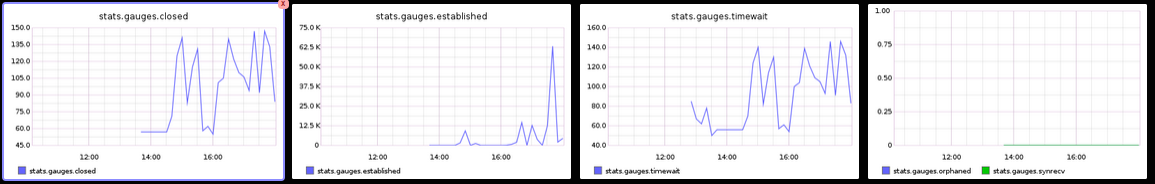
\includegraphics[scale=0.4]{graphitesocket}
\caption{Monitored TCP sockets.}
\label{figure:TCPstates}
\end{figure}

A very similar setup is also deployed in the cloud - a dedicated instance is running, to which all server instances send metrics in real-time.

\section{Nginx Optimizations}
On each WebSocket server instance, we are running an nginx process to end the encrypted communication and load balance traffic before all server processes running on a given machine.

The following optimizations were made to improve nginx performance. The fragment of the configuration can be found in listing \ref{lstlisting:nginx}.

\begin{description}
  \item [worker\_processes auto] sets the number of nginx processes to the number of available CPU cores automatically,
  \item [worker\_connections] sets the number of maximum connections opened by a worker process (cannot be higher than the number of allowed file descriptors per process),
  \item [TCP\_nodelay] setting to off disables Nagle’s algorithm and thus allows sockets not to buffer data but send it right away (and effectively reduce latencies by up to 0.2 seconds\footnote{\url{https://t37.net/nginx-optimization-understanding-sendfile-TCP\_nodelay-and-TCP_nopush.html}}),
  \item [TCP\_nopush] setting to off deactivates the TCP\_CORK option in the Linux TCP stack and allows to send smaller data chunks,
  \item [keepalive\_timeout] defines how long to keep an idle keep-alive connection open (in seconds),
  \item [proxy\_read\_timeout] defines how long to work for a backend to server the connection / request (high values necessary for potentially highly congested servers),
  \item [backlog] sets the max length of the queue of pending connections,
  \item [deferred] instructs the kernel not to wait for the final ACK packet and not to initiate the connection until the first packet of real data has arrived,
  \item [worker\_rlimit\_nofile] sets the limit of file descriptors that can be opened by nginx process (2 are necessary for each WebSocket connection - incoming and forwarded).
  \item [round-robin] routing had to be added to the WebSocket server upstream so that incoming connections are divided between all server processes.
\end{description}ś

\begin{sourcecode}[h]
\begin{lstlisting}[style=mono]
worker_processes auto;
worker_connections 165535;
TCP_nopush off;
TCP_nodelay off;
keepalive_timeout 1000;
proxy_read_timeout 1000;
worker_rlimit_nofile 30000;

upstream api_server_dev {
    server 127.0.0.1:9998;
    server 127.0.0.1:9997;
    server 127.0.0.1:9996;
    server 127.0.0.1:9995;
    server 127.0.0.1:9994;
    server 127.0.0.1:9993;
    server 127.0.0.1:9992;
    [...]
}

[...]
# inside server section
listen 443 backlog=16384 deferred;
[...]
\end{lstlisting}
\caption{Nginx configuration modifications.}
\label{lstlisting:nginx}
\end{sourcecode}

\section{MySQL Optimizations}
Most of MySQL optimizations are still ahead, since I haven't really stretched it to its limits yet. We have encountered and solved a massive bottleneck at one point. MySQL would periodically, regularly stall for a very long time.

I managed to pinpoint the issue down to the frequency with which the log was flushed to disk. With the default value of the \textit{innodb\_flush\_log\_at\_trx\_commit} parameter (1), this happens on every transaction commit. Since changing the parameter value to 2, the flushing only happens once per second and the performance has vastly improved.

The second parameter I modified is \textit{max\_connections} so that all the server processes with their multiple threads could connect without problems against (we hit the default limit rather early).

\begin{sourcecode}[h]
\begin{lstlisting}[style=mono]
max_connections = 500
innodb_flush_log_at_trx_commit = 2
\end{lstlisting}
\caption{MySQL configuration modifications.}
\label{lstlisting:MySQL}
\end{sourcecode}

There is definitely potential for further improvements in this scope.

\section{Redis Optimizations}
As with MySQL, I have hit one major redis roadblock regarding redis. At seemingly random points through trial benchmark runs, redis process would become unreachable by the WebSocket server instances.

The error reported by the server processes (listing \ref{lstlisting:redis2}) and pointed to the redis server log, where the issue was narrowed down to forking \ref{lstlisting:redis}.

\begin{sourcecode}[h]
\begin{lstlisting}[style=mono]
ResponseError: MISCONF Redis is configured to save RDB snapshots,
but is currently not able to persist on disk.
Commands that may modify the data set are disabled.
Please check Redis logs for details about the error.
\end{lstlisting}
\caption{Server process log.}
\label{lstlisting:redis2}
\end{sourcecode}

\begin{sourcecode}[h]
\begin{lstlisting}[style=mono]
[1772] 24 Jul 10:09:09.009 \# Can't save in background: fork: Cannot allocate memory
[1772] 24 Jul 10:09:15.020 * 1 changes in 900 seconds. Saving...
\end{lstlisting}
\caption{Redis server log.}
\label{lstlisting:redis}
\end{sourcecode}

Redis documentation \footnote{\url{http://redis.io/topics/faq}} provides a simple answer and it is changing the already described \texttt{overcommit\_memory} kernel flag to 1. It instructs the kernel to be "more relaxed" when allocating additional memory for a process.

\section{Cloud Baseline Preparations}\label{Cloud baseline preparations}
Moving the prepared infrastructure to the cloud proved a new set of challenges, rather underestimated in the beginning of the project. The challenges were different for client and server machines.

\subsection{Client Instances}
Simulating the clients is done using a node process which spins a number of sockets it is instructed to by the load test suite orchestrator. A sample bash process is executed on each client instance \ref{lstlisting:bashloadtest}, which starts the appropriate number of node processes (equal to the number of CPU cores on the client machine).

As I identified performing the preparations locally, the load test suite node process is mostly CPU-bound. The confusing issue in the cloud was that it was hard to foresee when the limits are reached, since they different depending on the general system load (with the increased load the number and size of broadcast messages the clients had to process increased as well).

I started the tests using t1.micro EC2 instances. Eventually I had to move to m1.small (these are the machines eventually used in the benchmark), because the processes were reaching memory limits when tests were run for longer than ~3 minutes. After hours of debugging (when the node process crashes on a remote instance, the load test master which orchestrates the suite receives no data whatsoever), I realized that the kernel was silently killing the node processes \ref{lstlisting:clientkernel}.

Because it was difficult the estimate resource limits, I decided to hugely over-provision client instances so that their resource limits are never reached and measurement of The System Under Test \ref{The System Under Test} are not affected in any undesirable way.

\begin{sourcecode}[h]
\begin{lstlisting}[style=mono]
Jul 24 11:36:28 ip-172-31-24-5 kernel: [39921901.888692] Out of memory:
"Kill process 2992 (node) score 673 or sacrifice child"
\end{lstlisting}
\caption{Load test client machine kernel log.}
\label{lstlisting:clientkernel}
\end{sourcecode}

Since most preparations were initially run on smaller scale (to save costs), the issues would generally manifest themselves only when the suite was deployed on a big scale.

\subsection{Image Preparations}
Both servers and clients are spun up using AMIs (Amazon Machine Images)\footnote{\url{http://docs.aws.amazon.com/AWSEC2/latest/UserGuide/AMIs.html}}, which contain all configuration for an instance deployable in the cloud. They are highly customizable and reusable. Client, server and database instanced required slightly different images. All had to be meticulously prepared and configured (using the techniques described in the sections above) to ensure smooth deployment, high performance and reliability.

Image configuration includes:
\begin{itemize}
  \item /etc/init.d and chkconfig entries to automatically start relevant services on instance start, such as sshd, redis server, MySQLd and supervisord (to start python WebSocket servers),
  \item internal system configuration containing all correct host-names for all system components (which differ between tested architectures),
  \item security groups defining open ports and protocols for inbound and outbound communication of an instance.
\end{itemize}

\subsubsection{Distributing Resources Across Cloud Regions}

Amazon AWS infrastructure is divided into Regions (e.g. Ireland, N. Virgina, Sao Paolo). These regions are further divided into availability zones \ref{figure:awsregions}.


Multiple availability zones very important in a shared cloud environment, because a single availability zone can become a single point of failure (for instance when another customer is getting hit by a DDoS \cite{GroBuy}).


\begin{figure}[H]
\centering
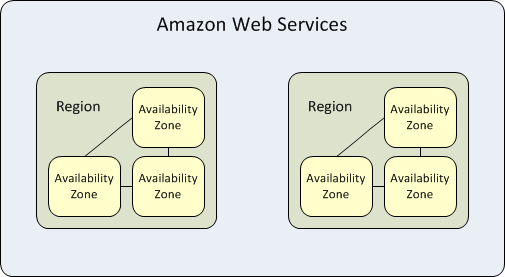
\includegraphics[scale=0.8]{awsregions}
\caption{AWS Regions and Availability zones.}
\label{figure:awsregions}
\end{figure}

Most of the service stack is prepared and registered with Amazon within a single region. There is no easy way to copy the prepare setup between regions, other than (in some cases) manually or using AWS API. I prepared a full set of python scripts utilizing Amazon-provided library, boto \footnote{\url{http://aws.amazon.com/sdk-for-python/}}, to distribute our AMIs, launch configurations, autoscaling groups and other services setup across the regions. The listing \ref{lstlisting:copygroups} contains a simplified script for copying autoscale groups between regions.

\begin{sourcecode}[H]
\begin{lstlisting}[style=mono, language=Python]
# A simplified version of copying autoscale groups
# between regions (simplified for the sake of brevity)
def copy_autoscale_group_between_regions(
    group_name, desired_group_count, dest_region,
    source_region, launch_config, routing_policy_data
  ):
  """Return a list of public IPs of the created instances of the new group.
  """

  # copy load balancers associated with group
  load_balancers     = im_boto.get_load_balancers_for_group(source_region, group_name)
  dest_load_balancers = []
  for elb in load_balancers:
    dest_elb = im_boto.get_load_balancer_by_name(dest_region, elb.name)
    if not dest_elb:
      dest_elb = im_boto.copy_load_balancers_between_regions(
        source_region, dest_region, elb
      )

      im_boto.register_new_load_balancer_with_route53(
        dest_elb, routing_policy_data,
        domain='route53.instamrkt.com'
      )
    dest_load_balancers.append(dest_elb)

  # create test scale group if not exists
  dst_group = im_boto.get_auto_scale_group_by_name(
     dest_region, group_name
  )
  if not dst_group:
    dst_launch_config = im_boto.get_launch_configuration(
      im_boto.autoscale_connections[dest_region], launch_config_name
    )
    if not dst_launch_config:
      dst_launch_config = im_boto.copy_launch_config_between_regions(
        source_region, dest_region, launch_config
      )

    dst_group = im_boto.create_auto_scaling_group_from_params(
      dest_region, group_name,
      dst_launch_config, dest_load_balancers
    )


  deployed_ips = im_boto.update_group_desired_capacity(
    im_boto.autoscale_connections[dest_region],
    group, desired_group_count
  )

  # here happens verification if all instances are reachable
  return deployed_ips
\end{lstlisting}
\caption{Copying Autoscale Groups between regions.}
\label{lstlisting:copygroups}
\end{sourcecode}

\subsubsection{Exluding Frankfurt Region}\label{Exluding Frankfurt Region}

Amazon offers 9 regions for auto scaling - 8 are listed in the Users Distribution section \ref{Users Distribution}, the 9th is Frankfurt. Because of technological limitations I was forced to exclude this region from my research.

The AMIs I use are not compatible with the region's infrastructure. Amazon offers two types of image virtualization: PV (paravirtual) and HVM (hardware virtual machine) \footnote{\url{http://docs.aws.amazon.com/AWSEC2/latest/UserGuide/virtualization_types.html}}. I use PVs, whereas Frankfurt has very limited support for them.

\section{Load Testing Framework}\label{Load Testing Framework}
The load testing framework consists of the following components:

\subsubsection{General Load Test Orchestration Script}
This python script command the whole benchmark execution. Its steps are listed in the pseudo-code listing \ref{lstlisting:orchestration}. Written by me.

\begin{sourcecode}[H]
\begin{lstlisting}[style=mono]
Copy load test client setup from source region to all destination regions.
Start up the desired number of client instances in each region.
Copy server setup from source region to all destination regions.
Start up the desired number of server instances in each region.
Collect public IP addresses of all deployed client, server, MySQL and redis instances.
For each client IP address, spawn a node remote access process sending
the "start load test" command and parameters.
Sleep for the desired benchmark run length.
For each client IP address, spawn a node remote access process sending
the "stop load test" and "collect metrics" command and parameters.
For each server IP address, collect server side metrics.
For each redis IP address, collect redis metrics.
For each MySQL IP address, collect MySQL metrics.
\end{lstlisting}
\caption{Benchmark run orchestration script pseudo-code.}
\label{lstlisting:orchestration}
\end{sourcecode}

\subsubsection{Remote Access + Start Test Process} This node script connects to the remote machine using the node sequest library \footnote{\url{https://github.com/mikeal/sequest}}, which utilizes the local ssh-agent to authenticate with the remote host. Listed in full below \ref{lstlisting:remotestart}. Written by me.

\begin{sourcecode}[H]
\begin{lstlisting}[language=javascript]
#!/usr/bin/env node

var sequest = require("sequest");

// receives cmd line parameters from the
// benchmark orchestration python script
var host            = process.argv[2],
    processes       = process.argv[3],
    usersPerProcess = process.argv[4],
    concurrentUsers = process.argv[5],
    startUserId     = process.argv[6];

var user      = "lukasz";
var remoteDir = "/opt/web/dev-instamrkt/utils/scaling/load_testing/";

function executeRemoteLoadTestClient(host) {
  var cmd = "cd " + remoteDir + " && ./perform_load_test_from_multiple_processes.sh "
    + processes + " " + usersPerProcess + " " + concurrentUsers + " " + startUserId;

  sequest(user + "@" + host, cmd, function (e, stdout) {
    if (e) throw e;
    console.log("Execution started.");
  });
}

executeRemoteLoadTestClient(host);

\end{lstlisting}
\caption{Remote load test start script.}
\label{lstlisting:remotestart}
\end{sourcecode}

\subsubsection{Remote Access + Stop Test And Collect Metrics Process}
Very similar to the previous script. Sends the kill signal, sleeps a bit (so that the load test process can finish processing messages and summary metrics), collects remote metrics and saves them locally. Listed in full below \ref{lstlisting:remotestop}. Written by me.

\begin{sourcecode}[H]
\begin{lstlisting}[language=javascript]
#!/usr/bin/env node

// https://github.com/mikeal/sequest

var sequest = require('sequest'),
    fs      = require('fs');

// receives cmd line parameters from the
// benchmark orchestration python script
var host          = process.argv[2],
  processes       = process.argv[3],
  localDir        = process.argv[4];

var user          = "lukasz";
var remoteDir     = "/tmp/";
var waitAfterKill = 120;            // in seconds

var seq    = sequest(user + "@" + host);

function stopRemoteLoadTestClient() {
  seq.write("killall node", "", function(e) {
    if (e) {
      console.log(e);
    }
    else {
      // remote process killed - sleep a bit to
      // let it finish processing and saving metrics

      setTimeout(function() {
        for (var i=1; i <= processes; i++) {
          var fileName   = i;
          var reader     = sequest.get(user + '@' + host, remoteDir + fileName);
          var fileHandle = fs.createWriteStream(localDir  + '/' + fileName);

          reader.pipe(fileHandle); // reader.pipe(process.stdout) - to write to stoud
        }
      }, waitAfterKill * 1000);
    }
  });
}

stopRemoteLoadTestClient();

\end{lstlisting}
\caption{Remote load test start script.}
\label{lstlisting:remotestop}
\end{sourcecode}

\subsubsection{Start Load Test Processes Bash Script}
Starts multiple node load test processes so as to utilize all available CPU cores. It is called from the Start Test script above. Shown in full on listing \ref{lstlisting:bashloadtest}. Written by me.

\begin{sourcecode}[H]
\begin{lstlisting}[style=mono, language=bash]
#!/bin/bash

# sample usage:
# ./connect_multiple.sh 3 100 50 300
# 3 processes, 100 users each, 50 a second, start with user_id = 300

args=("$@");
PROCESSES=${args[0]};
USERS_PER_PROCESS=${args[1]};
CONCURRENT_PER_PROCESS=${args[2]};
START_USER_ID=${args[3]};

USER_ID=$START_USER_ID
for i in $(seq 1 $PROCESSES); do
  USER_ID=$((USER_ID+USERS_PER_PROCESS))
  node WebSocket-bench/ \
      -a $USERS_PER_PROCESS \
      -c $CONCURRENT_PER_PROCESS \
      -u $USER_ID \
      -k -t classic wss://route53.instamrkt.com:443 > /tmp/$i &
done

echo "All started."

\end{lstlisting}
\caption{Bash process commanding the load test execution on a single machine.}
\label{lstlisting:bashloadtest}
\end{sourcecode}


\subsubsection{Load Test Process}
This is by far the most complex of all pieces. It is a rather complex node process with multiple simulated workers. It supports arbitrary numbers of users and an arbitrary number of them connecting every second. It also supports keep-alive connections which I use during the benchmark run. It is based on 3rd party package, WebSocket-bench\footnote{\url{https://www.npmjs.com/package/WebSocket-bench}}. Surprisingly, the library does not support the WebSocket library I use, a de-facto standard node WebSocket library\footnote{\url{https://github.com/WebSockets/ws}}. I heavily extended the WebSocket-bench library and hope to integrate my development when the code is polished.

The script opens concurrent WebSocket connections, sends and receives messages according to the configured scenario (which I coded and integrated), and upon completion (receiving the kill signal in case of keep-alive connections) generates a metric report. I extended the metric report with custom reporting basing on the fast-stats module\footnote{\url{https://github.com/bluesmoon/node-faststats}}.

Listings \ref{lstlisting:loadtestexec}, \ref{lstlisting:loadtestexec2}, \ref{lstlisting:loadtestexec3}, \ref{lstlisting:loadtestexec4},  show different, crucial parts of the load test code base.

\begin{sourcecode}[H]
\begin{lstlisting}[language=javascript]
// Creates all necessary workers
Benchmark.prototype.launch = function (connectNumber, concurency, workerNumber, nbMessage) {
  var cp = require('child_process');
  // ...
  for (var i = 0; i < workerNumber; i++) {
    this.workers[i] = cp.fork(__dirname + '/worker.js', [
      this.server, this.options.generatorFile, this.options.type,
      this.options.transport, this.options.verbose, this.options.userId
    ]);
    this.workers[i].on('message', this._onMessage.bind(this));
  }
  this._nextStep(concurency, connectNumber, concurency, nbMessage);
};
\end{lstlisting}
\caption{Create necessary workers.}
\label{lstlisting:loadtestexec}
\end{sourcecode}

\begin{sourcecode}[H]
\begin{lstlisting}[language=javascript]
// Opens a specified number of connections every second
Benchmark.prototype._nextStep = function (currentNumber, connectNumber, concurency, nbMessage) {
  for (var i = 0; i < this.workers.length; i++) {
    var nbConnection = Math.round(concurency / this.workers.length);
    if (i === this.workers.length - 1) {
      nbConnection = concurency - nbConnection * i;
    }
    this.workers[i].send({ msg : 'run', number : nbConnection, nbMessage : nbMessage});
  }
  if (currentNumber < connectNumber) {
    setTimeout(function () {
      if (currentNumber >= connectNumber - concurency) {
        concurency = connectNumber - currentNumber;
        currentNumber = connectNumber;
      } else {
        currentNumber += concurency;
      }
      _this._nextStep(currentNumber, connectNumber, concurency, nbMessage);
    }, 1000);
  }
};
\end{lstlisting}
\caption{Open a specified number of connections each second until total number reached.}
\label{lstlisting:loadtestexec2}
\end{sourcecode}

\begin{sourcecode}[H]
\begin{lstlisting}[language=javascript]
// creates a single connection
ClassicWorker.prototype.createClient = function (callback) {
  var connection      = new WebSocket(options.url);
  connection.init     = Date.now();

  connection.onopen = function (session) {
    _this.metrics.handshaken({'duration': Date.now() - connection.init});
    _logOn();
    callback(false, session);
  }; // .... All handlers and messaging scenario registered below
}
\end{lstlisting}
\caption{Create a single WebSocket client.}
\label{lstlisting:loadtestexec3}
\end{sourcecode}

\begin{sourcecode}[H]
\begin{lstlisting}[language=javascript]
process.on('SIGINT', function () { // Intercept Kill Signal
  _.each(workers, function(worker) { worker.close();});
  metrics.established().stop().summary();
  setTimeout(function () { process.exit();}, 6000);
});

\end{lstlisting}
\caption{Intercept kill signal and save collected metrics.}
\label{lstlisting:loadtestexec4}
\end{sourcecode}


\subsection{Tool Selection}

Before I settled for the load testing library, I analyzed multiple different tools. My two main criteria were: it needs to extensible (since I need to introduce my on testing scenarios) and understandable, preferably the technology I know (so that I can work with it on a tight deadline).

The analyzed tools include:
\begin{description}
  \item [JMeter]- Java-based, difficult to set up and not customizable\footnote{\url{https://github.com/maciejzaleski/JMeter-WebSocketSampler}},
  \item [thor]- node-based, low extensibility\footnote{\url{https://github.com/observing/thor}},
  \item [autobahn]- python-based, designed with different use-cases in mind\footnote{\url{http://autobahn.ws/testsuite/}},
  \item [tsung]- erlang-based, very low community support, bad documentation, couldn't get my head around it quickly enough\footnote{\url{http://tsung.erlang-projects.org/}}.
\end{description}

None of the tools met the extensibility and understandability criteria as well as WebSocket-bench.

\subsection{Making Load Test Process Bulletproof}
This was absolutely necessary. If the process has failed, no results would be reported and the master node would be in the dark as to what happened on the client machine where the load test process failed.

In the investigation process, I have identified and protected against 3 main uses:

\begin{enumerate}
  \item Client writing to a closing socket would cause the process to crash. This would happen when client was simulating many sockets and the kill signal would be received - sockets would be closed but, according to the configured scenario, message was to be sent at this very moment. Adding a check of the socket state before writing solved to issue.
  \item When deploying at scale (120 client machines), the test master would sometimes experience an ssh-timeout when connecting to the client machine. This was happening because the master connects to all clients at the same time and processing of each takes some time. Increasing the timeout value to 999999 in the sequest library configuration solved the issue.
  \item Sending the kill signal would in a few percent of cases cause the load test process to crash. This happened extremely rarely in a non-deterministic fashion. The protection against it has been put in place (not the most advisable one from a software engineering standpoint, yet reliable and this was the goal) and is shown in listing \ref{lstlisting:errorcatch}. Since node is an inherently asynchronous environment, using \textit{try..catch} blocks to narrow down the scope of where the error was happening was not possible.
\end{enumerate}

\begin{sourcecode}[H]
\begin{lstlisting}[language=javascript]
process.on('uncaughtException', function(err) {
    console.log('Exception:', err)
});
\end{lstlisting}
\caption{Catch any exception inside to load test node process.}
\label{lstlisting:errorcatch}
\end{sourcecode}

\section{Compared Architectures Implementation Details}\label{Compared Architectures Implementation Details}

I was somewhat limited in EC2 instance type selection, since not all instance types support the type of AMI I was using. Nevertheless, I selected the instance types so that all tested architecture decompositions have similar total amounts of resources allocated (to the best possible extent).

For WebSocket server instances (and redis where applicable), I picked CPU-optimized instance types because by far this is the first hardware limit the System Under Test \ref{The System Under Test} was reaching at any scale during preparations.

\subsection{Baseline Architecture Implementation Details}\label{Baseline Architecture Implementation Details}

This Architecture consists of a single server machine. The instance type selected for this was a c3.8xlarge\footnote{\url{https://aws.amazon.com/ec2/instance-types/}} - 32 CPU cores, 60GB of RAM, 140GB of SSD storage with 4000 provisioned IOPS\footnote{Even though the tested application does not need all the storage space, I needed to provision that much since Amazon requires a ratio no bigger than 30 between the number of provisioned IOPS (which is what I wanted to be high) and the disk size.}.

The machine hosts:
\begin{itemize}
  \item the nginx server with automatically adjusted number of workers,
  \item the WebSocket API processes - 16, one for every 2 available CPU cores,
  \item the MySQL server,
  \item the redis server (single thread).
\end{itemize}

This architecture introduces no network overhead in terms of communication between system components, yet clients from across the globe have to connect to the remote server.

All processors at the EC2 instances are of type Intel Xeon E5-2680 v2 \footnote{\url{http://ark.intel.com/products/75277/Intel-Xeon-Processor-E5-2680-v2-25M-Cache-2_80-GHz}}.

\subsection{Proposed Architecture I Implementation Details}\label{Proposed Architecture I Implementation Details}

This Architecture consists of a 8 server machines (one per each region where clients connect from), single big redis and single big MySQL instances. Database instances are located in Ireland.

Each server is running on an m3.xlarge instance \footnote{\url{https://aws.amazon.com/ec2/instance-types/}} - 4 CPU cores, 15GB of RAM, 140GB of SSD storage with 4000 provisioned IOPS (in order to be able to reuse the server AMI this was the minimal amount of storage).

Each server machine hosts:
\begin{itemize}
  \item the nginx server with automatically adjusted number of workers,
  \item the WebSocket API processes - 2, one for every 2 available CPU cores.
\end{itemize}

As a database solution, this architecture uses 1 big redis instance - m2.xlarge, 1 core (since I am running one-redis process anyway), 17.1 GB mem and 140GB of SSD storage with 4000 provisioned IOPS and a 1 big MySQL RDS instance (r3.4xlarge, 16 cores, 122 GB mem) and 100 GB disk 1000 IOPS\footnote{RDS IOPS/disk size max ratio is 10:1, so I decided to trade-off cost of a 400GB disk (that is what is necessary for 4000 IOPS on RDS) for lower IOPS value (which is not expected to be a limitation anyway - observed values were below 500 IOPS).}.

\subsection{Proposed Architecture II Implementation Details}\label{Proposed Architecture II Implementation Details}

This Architecture consists of 8 server machines (one per each region where clients connect from), 1 one big master redis write instance, 1 big MySQL write RDS instance and 8 MySQL RDS read replicas (one per region). Redis also has read replication nodes, they are physically located at the same machines as the WebSocket servers. Database master instances are located in Ireland.

Each server machine hosts:
\begin{itemize}
  \item the nginx server with automatically adjusted number of workers,
  \item the WebSocket API processes - 2,
  \item the redis server, a read-only slave of a writable master (single thread).
\end{itemize}

Each server and redis read replica instance is running on an m3.2xlarge instance\footnote{\url{https://aws.amazon.com/ec2/instance-types/}} - 8 CPU cores, 30GB of RAM, 140GB of SSD storage with 4000 provisioned IOPS (again, in order to be able to reuse the server AMI this was the minimal amount of storage). This is a slight over-provision, yet I have not increased the number of running WebSocket server processes so as to have a fair comparison to other architectures. The over-provisioning results from the fact that necessary CPU cores were needed so that redis server and WebSocket servers don't clash at one core.

Redis write master is using an m2.xlarge - 1 core with 17.1 GB of RAM. MySQL master RDS node uses db.r3.2xlarge instance - 8 cores with 61GB of RAM. Each MySQL read replica node is using a db.m3.medium (1 CPU core, 3.75 GB RAM) instance.

Amazon introduces another limitation - no more than 5 read replicas per master. That made our setup slightly asymmetrical - Irish WebSocket servers connect directly to master instances, and Sydney's MySQL reads from a replica located in Singapore, and California reads from replica located in Oregon as depicted on the figure \ref{figure:archprop2}. Chaining up to 3 replicas is allowed, but no more than 1 cross-region boundary can be included in the chain\footnote{\url{http://docs.aws.amazon.com/AmazonRDS/latest/UserGuide/USER_ReadRepl.html\#USER\_ReadRepl.XRgn}}. That means that a chain Ireland -> Singapore -> Sydney is not allowed.

\section{Cloud architecture setup} \label{Cloud architecture setup}
The cloud architecture stack consists of the following:
\begin{itemize}
  \item Route53 \ref{Route53}, routing users between server instances,
  \item Nginx, routing users server processes within a single instance,
  \item stateless WebSocket servers,
  \item redis databases,
  \item MySQL databases.
\end{itemize}

Originally, Route53 was routing users through Elastic Load Balancers. This was not used in the benchmarking process, as explained below \ref{Load balancing}.

\begin{figure}[H]
\centering
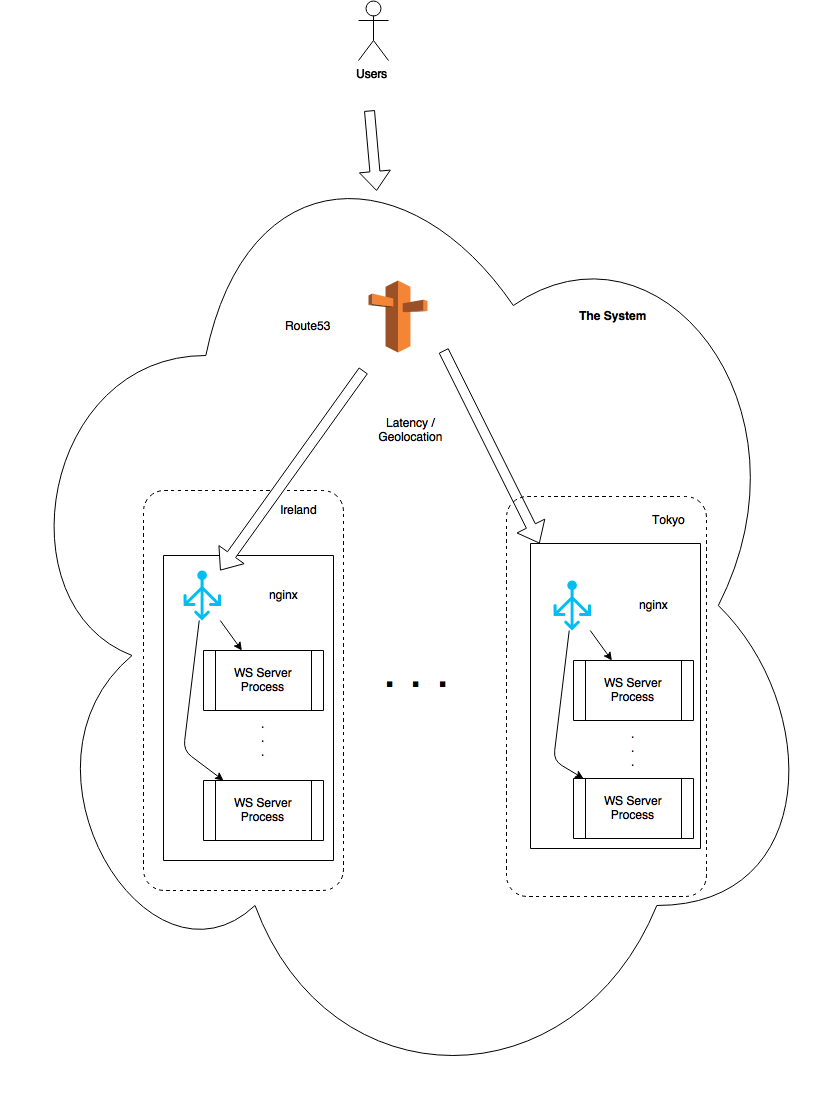
\includegraphics[scale=0.4]{cloudsetup}
\caption{How users are server by the system in the cloud.}
\label{figure:cloudsetup}
\end{figure}

\subsection{Route53}\label{Route53}

Route53 is Amazon's cloud-based DNS web service\footnote{\url{https://aws.amazon.com/route53/}}. I use it to map a single URL to which all clients connect to, \texttt{route53.instamrkt.com}, to currently deployed server instances. The mapping can point to multiple public EC2 instance IP addresses (which is what I am using) or public DNS names (e.g. of Load Balancers with varying number of server instances behind them).

Route53 offers different routing policies:

\begin{description}
  \item[Simple] redirects all queries to a single service point (e.g. web server) behind it,
  \item[Weighted] routes the queries queries behind multiple resource end points in proportion to weights specified for the resources,
  \item[Latency Based] uses the latency between the resource endpoints and the requesting client to select the endpoint. Amazon is only specific enough to say that in this process they use a "latency measurements performed over time" \footnote{\url{http://docs.aws.amazon.com/Route53/latest/DeveloperGuide/routing-policy.html}},
  \item[Failover] routes all queries to one end point and only if that one fails to other backup end points,
  \item[Geolocation] routes users based on geographic location. Route53 offers configuring Geo-location routing on following levels: state(only for USA), country, continent and global. For each end user’s location, Route 53 will return the most specific Geo DNS record that includes that location. In other words, for a given end user’s location, Route 53 will first return a state record; if no state record is found, Route 53 will return a country record; if no country record is found, Route 53 will return a continent record; and finally, if no continent record is found, Route 53 will return the global record.
\end{description}

For the benchmarking (in cases where routing between servers was needed), I used Latency Based Routing. I compared it against Geo-location routing and found no meaningful differences - clients go through Route53 only during initial handshake and geographical proximity to the server was highly inversely correlated with the latency to the server.

The service also offers health checks, which can be used custom-defined or picked up from other services such as load balancing. Users will only be routed to end points configured "healthy"\footnote{\url{http://docs.aws.amazon.com/Route53/latest/DeveloperGuide/dns-failover-complex-configs.html}}.

\subsection{Autoscaling}

Autoscaling is Amazon's service that helps to scale the application capacity up and down according to configurable conditions\footnote{\url{http://aws.amazon.com/autoscaling/}}. Each group has a launch configuration associated with it, which specifies what an instance that is supposed to be added when scaling up should look like (instance type, AMI, security group etc.).

Autoscaling group capacity can be changed automatically according to a scaling policy. Scaling policy specifies how to automatically change group capacity (\textit{add/remove/set to} a number of instances) in reaction to an alarm. An alarm is an object that watches over a single metric (e.g. avg CPU use of ec2 instances in the auto scaling group over specified time period). In general, the recommendation is to use one policy for scaling out, another policy for scaling in.

I use autoscaling groups both for clients and servers. It helps with orchestrating the architecture, benchmarking and most importantly with dynamic scaling up and down. The last, even though implemented by me, is outside of scope for this project because of the issues explained in section \ref{Excluded Metrics} and \ref{System Scaling Delay}.

\subsection{Elastic Load Balancing}\label{Load balancing}
Elastic Load Balancing is a service automatically distributing incoming traffic between multiple server instances. An Elastic Load Balancer can be associated with an autoscaling group so that new instances can be added or the old ones removed, and that process remains invisible to other parts of the system which reaches server instances through ELB's public DNS name. For TCP requests, the only routing policy Load Balancers offer is round robin\footnote{\url{ttp://docs.aws.amazon.com/ElasticLoadBalancing/latest/DeveloperGuide/how-elb-works.html\#request-routing}}.

Elastic Load Balancers do not expose a public IP address, since internally they are implemented as multiple physical machines. The number of nodes (machines) provisioned for a load balancer varies depending on traffic and \texttt{cannot be directly configured}. Amazon uses internal heuristics to determine how many instances to provide. The only way to pre-warm to load balancers when expecting traffic surges (such as a load test) is to contact appropriate support teams within Amazon. This proved to be highly problematic - I couldn't run the full load benchmark right away, but had to slowly, incrementally increase the traffic to give load balancers a chance to scale up. I spent hours investigating this process, together with Amazon's support. Furthermore, if a load balancer does not receive sufficient traffic over a period for 12 hours, it scales down completely. That means that the whole processes would need to be essentially repeated for each benchmark run. Because of all this, I decided to give up usage of Elastic Load Balancing. I could make this decision, because issues with the DNS protocol (\ref{System Scaling Delay} and \ref{Excluded Metrics}) made it impossible to measure speed of dynamic scaling of the application.

\begin{figure}[H]
\centering
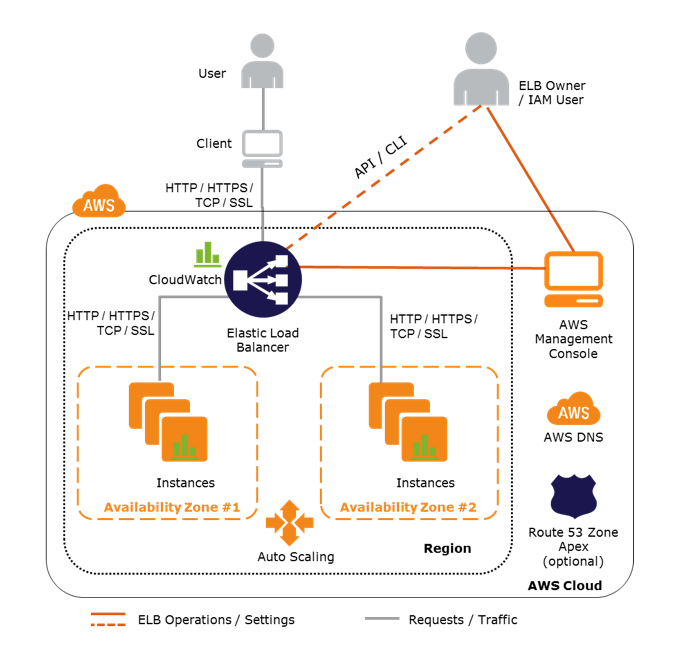
\includegraphics[scale=0.5]{elbautoscale}
\caption{How Elastic Load Balancing works with Auto Scaling.}
\label{figure:elbautoscale}
\end{figure}

\subsection{Data Layer}
As the tested system \ref{The System Under Test} uses MySQL and reds as database solutions, I investigated and used (to the highest possible extent), the services that Amazon offers in that scope.

Amazon Solution Architects, whom I was consulting throughout this project, suggested using technologies like DynamoDB and Kinesis instead of the redis + MySQL setup the application currently uses. Both will be looked into but are out of scope for this project.

\subsubsection{Amazon Relational Database Service}

RDS is Amazon's solution for relational databases, such as MySQL. When it comes to cross-region support, it has its huge limitations. MySQL cluster cannot be deployed in a multi-region setup. Effectively, the only cross-region supported topology is a single writable master with globally distributed read replicas. I used this setup in the 3rd tested architecture \ref{Proposed Architecture II}.

\subsubsection{Elasticache}

Elasticache\footnote{\url{https://aws.amazon.com/elasticache/}} is Amazon’s in-memory cache scalable solution. It supports memcached and redis. Grozev and Buyya suggest using it \cite{GroBuy}. Sadly, Elasticache is only usable within one region, which renders it useless for the purpose of this research.

In the research, custom redis master-slaves topology is used. Setting up a topology like this is extremely easy: as soon as a redis server receives a command \texttt{slaveof HOSTNAME PORT} it becomes a non-writable, automatically synchronized read replica of the master located at \texttt{HOSTNAME:PORT}.

\section{System Scaling Delay}\label{System Scaling Delay}
Measuring the speed of scaling up and down proved to be very difficult and was eventually excluded from this research. The following factors constitute the perceived system scaling delay:
\begin{description}
  \item [Cloudwatch] - even in a detailed mode (which offers metrics collectible every 1 minute instead of every 5 minutes), the delay of received metrics during our tests averaged out at ~2 minutes. That means that every scale in / out action that could be undertaken is delayed at least by that time.
  \item [DNS protocol issues] - a huge number of DNS servers do not obey TTLs (time-to-live) on DNS records. Therefore, there is no guarantee that even a record with a TTL set to 60 seconds becomes updated every minute for all, globally distributed, clients. I tested this empirically and my research lead me to conclusion that this is a known issue in the community\footnote{\url{http://engineering.chartbeat.com/2014/01/02/part-1-lessons-learned-tuning-TCP-and-nginx-in-ec2/}}. There is simply no way to estimate when clients of the system are going to "see" the updates in a system topology.
\end{description}


%%%%%%%%%%%%%%%%%%%%%%%%%%%%%%%%%%%%%%%%%%%%%%%%%%%%%%%%%%%%%%%%%%%%%%%%%%%%%%%%

%%%%%%%%%%%%%%%%%%%%%%%%%%%%%%%%%%%%%%%%%%%%%%%%%%%%%%%%%%%%%%%%%%%%%%%%%%%%%%%%
\chapter{Experiment results}\label{Experiment results}

\epigraph{"You can't always get what you want, but if you try sometimes you just might find
you get what you need."}{--- The Rolling Stones}

\section{Executed Benchmark Overview}

Each architecture was tested using the benchmark load specified in table \ref{table:benchload}.

\begin{table}[H]
\begin{center}
\begin{tabular}{llll}
  \texttt{Value}          & \texttt{Each Client Machine}        & \texttt{Number of Client Machines}  & \texttt{Total}\\
  \hline
  Total concurrent users  & 200                         & 120                         & 24000         \\
  Connecting per second   & 1                           & 120                         & 120           \\
\end{tabular}
\end{center}
\caption{Benchmark user load.}
\label{table:benchload}
\end{table}

Benchmark run lasted exactly $200 + 90 * 60 = 5600s (93.3min)$ and its message load is specified in table \ref{table:benchload2}.

\begin{table}[H]
\begin{center}
\begin{tabular}{llll}
  \texttt{Value}          & \texttt{Total Number}        & \texttt{One per period of (s)} \\
  \hline
  Average number of requests per user  & 350   & 21\\
  Average number of received broadcast messages  & 1800   & 3                     \\
\end{tabular}
\end{center}
\caption{Benchmark message load.}
\label{table:benchload2}
\end{table}

\section{Sample Client Report}\label{Client Report}
Each client generating load during the benchmark run provides a report like the one on listing REF.

\begin{sourcecode}[H]
\begin{lstlisting}[language=json]
Launch bench with 10 total connection, 1 concurent connection
0 message(s) send by client
1 worker(s)
WS server : classic


On-line               188118 milliseconds
Time taken           188118 milliseconds
Connected            10
Disconnected         0
Failed               0
Collected from:      10

Durations (ms):

                     min     mean     stddev  median     max sampleCount
Handshaking          12      58           52      31     158      10
Latency              11      19            4      19      38     154
Broadcast Latency    7       9             1       9      17     409

Percentile (ms):

                      50%     66%     75%     80%     90%     95%     98%     98%    100%
Handshaking          31      79      97      116     158     158     158     158     158
Latency              19      20      20      20      21      26      33      35      38
Broadcast Latency    9       10      10      10      11      12      13      14      17
\end{lstlisting}
\caption{A sample single client load test report (latencies in milliseconds).}
\label{lstlisting:prediction}
\end{sourcecode}

\section{Sample Server Report}
Each metric for each server is reported in a separate CSV file \ref{lstlisting:memutilsrv}. The metrics are collected with the finest granularity possible - every 1 minute. This is why minimum, average, maximum and sum values do not differ. They would only if the requested data granularity was bigger than collection granularity - in my case both are equal 1 minute.

Each server metric calculation are based on 94 data points - for 94 minutes of the benchmark, starting at the minute when the benchmark run was started.

\begin{sourcecode}[H]
\begin{lstlisting}[style=mono]
Timestamp,Average,Maximum,Sum,SampleCount,Unit
2015-08-05 10:06:00,3.44471529408956,3.44471529408956,3.44471529408956,3.44471529408956,1.0,Percent
2015-08-05 10:08:00,3.44489694659014,3.44489694659014,3.44489694659014,3.44489694659014,1.0,Percent
2015-08-05 10:07:00,3.44405355998029,3.44405355998029,3.44405355998029,3.44405355998029,1.0,Percent
2015-08-05 10:09:00,3.44695999998962,3.44695999998962,3.44695999998962,3.44695999998962,1.0,Percent
2015-08-05 10:10:00,3.44849107106596,3.44849107106596,3.44849107106596,3.44849107106596,1.0,Percent
\end{lstlisting}
\caption{A sample server memory utilization report.}
\label{lstlisting:memutilsrv}
\end{sourcecode}

\subsection{Cloudwatch metrics discrepancy}

For some metrics, such as memory or disk usage, Cloudwatch offers utilization (\%), available total and used total quantity. I have noticed that there exist some discrepancies between the 3 values. An example can be found in listing \ref{lstlisting:clouddiscr}. Cloudwatch reports 3123.859375 used and 57097.76953125 available memory. The ratio of these values is equal $3123.859375 / 57097.76953125 = 0,05471070763$, yet utilization reports 5.187\% instead of 5.471\%. This is why I decided \texttt{not} to use utilization values, and compute ratios for each of the metric. This is necessary for computing system averages anyway - to compute average deployed system memory utilization, I cannot average out the utilization percentages - all available values of all instances have to be added together, as do used values, and then a ratio of \textit{total used/total available} can be computed.

\begin{sourcecode}[H]
\begin{lstlisting}[style=mono]
# Memory utilization
Timestamp,Average,Maximum,Sum,SampleCount,Unit
2015-07-24 17:58:00,5.18727146996151,5.18727146996151,5.18727146996151,5.18727146996151,1.0,Percent

# Memory available
Timestamp,Average,Maximum,Sum,SampleCount,Unit
2015-07-24 17:58:00,57097.76953125,57097.76953125,57097.76953125,57097.76953125,1.0,Megabytes

# Memory used
Timestamp,Average,Maximum,Sum,SampleCount,Unit
2015-07-24 17:58:00,3123.859375,3123.859375,3123.859375,3123.859375,1.0,Megabytes
\end{lstlisting}
\caption{Cloudwatch reporting discrepancy.}
\label{lstlisting:clouddiscr}
\end{sourcecode}

\section{Results and interpretation}

Full experiment results are available on-line\footnote{\url{https://github.com/haren/UvA_Thesis/tree/master/thesis/results}}.

\subsection{Cloud Resources Utilization}
To compared deployed architectures resource utilization, I use the \textit{Computing Resource Utilization Meter}.

The meter has a value for every of the 94 measured system states. Every minute the following values are input into the meter:
\begin{itemize}
  \item \texttt{Server CPU Utilization}, compiled over all server instances + redis + MySQL RDS instances, for each instance $utilization percentage * number of cores$ is taken into computation (all processors are of the same speed - 2.8GHz), so the exact formula looks like this: $$util_{avg} = \sum_{i=1}^{n}(c*u) / \sum_{i=1}^{n}c$$ where $n$ is the number of instances, $c$ a number of cores on a given instance and $u$ utilization percentage of a given instance CPU.
  \item \texttt{Memory Utilization}, compiled over all server instances + redis instances, computed as sum of total used memory divided by sum of total available memory,
  \item \texttt{Disk Utilization}, compiled over all server instances + redis instances, computed as sum of total used disk space divided by sum of total available disk space.
\end{itemize}

It is worth noting that this means that the minimum CRUM value does not have to be comprised of minimum CPU, memory and disk utilizations. This would be the case only and only if all the minima happen at the same point in time.

Each input is equal to the percentage value -so if a utilization is equal 15.52\%, the input will be 15.52. Results for the 3 compared architectures are presented in table \ref{table:crum}.

\begin{table}[H]
\begin{center}
\begin{tabular}{llll}
  \texttt{Value}          & \texttt{Baseline}   & \texttt{Proposed I}  & \texttt{Proposed II} \\
  \hline
  CPU min                 & 1.41000             & 0.16000              & 0.99950              \\
  CPU avg                 & 15.41234            & 4.72781              & 5.89334              \\
  CPU max                 & 17.57000            & 5.45352              & 6.63933              \\
  Available               & 32 * 2.8GHz         & 50 * 2.8GHz          & 73 * 2.8GHz          \\
  \hline
  Memory min              & 6.46433             & 3.69206              & 3.54456              \\
  Memory avg              & 13.40652            & 3.96222              & 4.34030              \\
  Memory max              & 18.21367            & 4.00332              & 4.90962              \\
  Available               & 53.13884(+/- 3GB)   & 31(+/- 0.1GB)        & 24(+/- 2.3GB)        \\
  \hline
  Disk min                & 15.50860            & 14.58213             & 14.32463             \\
  Disk avg                & 16.55431            & 14.58421             & 14.37806             \\
  Disk max                & 18.64203            & 14.58616             & 14.43662             \\
  Available               & 118(+/- 3GB)        & 240(+/- 0.01GB)      & 1082 (+/- 0.5GB)     \\
  \hline
  \texttt{CRUM min}       & 56.82622            & 24.74547             & 29.71976             \\
  \texttt{CRUM avg}       & \texttt{298.30941}  & \texttt{63.04514}    & \texttt{74.87883}    \\
  \texttt{CRUM max}       & 414.57287           & 69.02704             & 85.63872             \\
\end{tabular}
\end{center}
\caption{Resource utilization (all values in \%).}
\label{table:crum}
\end{table}

As the results show, the utilization resource is fairly low in all cases. Differences in allocated resources result from different infrastructure needs for each of the architectures. Baseline architecture performs best by far - average CRUM value of 298.30941, followed by Proposed architecture II with 85.63872 and Proposed I with 63.04514, as graphed on figure \ref{figure:crum}.

\begin{figure}[H]
\centering
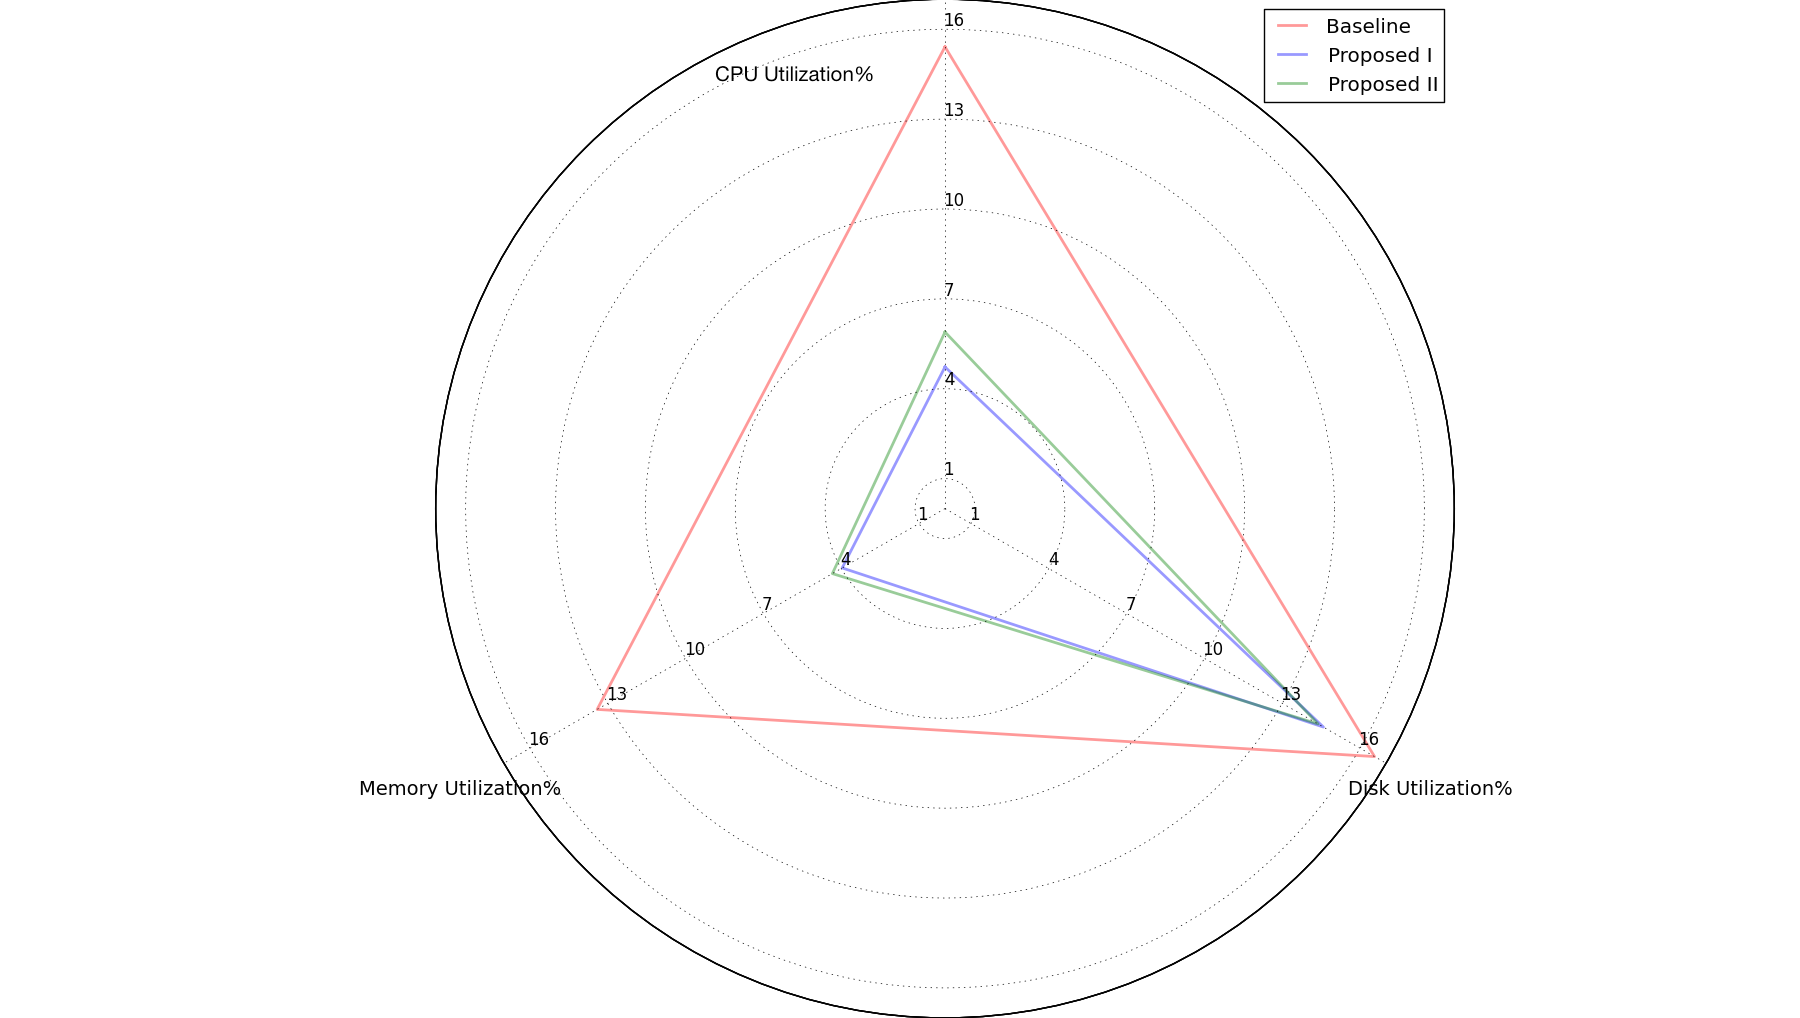
\includegraphics[scale=0.3]{crum}
\caption{CRUM meter comparison (the bigger the area the better).}
\label{figure:crum}
\end{figure}

\subsection{System Performance}
To compared performance of the deployed architectures, I use the \textit{System Performance Meter}.

The meter uses following metrics as inputs:
\begin{itemize}
  \item \texttt{handshaking latency} - a weighted average of all reports of all clients, reverse of minimum, average and 98th percentile values,
  \item \texttt{request handling latency} - a weighted average of all reports of all clients, reverse of minimum, average and 98th percentile values,
  \item \texttt{broadcast latency} - a weighted average of all reports of all clients, reverse of minimum, average and 98th percentile values,
  \item \texttt{network data in} - this is measured collectively over all server, redis and MySQL instances in the deployed system. It includes system internal data transfers. This is important because this is the data that is billable.
  \item \texttt{network data out} - this is measured collectively over all server, redis and MySQL instances in the deployed system. It includes system internal data transfers. This is important because this is the data that is billable.
\end{itemize}

There are a few remarks that need to be made regarding the input metrics. Since I observed that the latencies have a long-tailed distribution, I decided to use 98th percentile value as the upper value rather than the absolute maximum.

Because each client provides a separate report consisting (among others) of the mean and standard deviation, but not of the full data set, and because the deviations are relatively similar, pooled variance and standard deviation were computed for the global set of client-reported latencies. Since high latencies are undesirable, the reverse of measured latencies is input into the meter.

Since clients only report after the benchmark is finished, I do not have the benefit of providing a value of the meter for every minute of the benchmark run (as is the case with CRUM). The average values can provide comparison between architectures.

Another fact that is noticed during the analysis of client reports, is that standard deviations were consistently higher than the means in all of the reported sets. This was originally surprising, since latencies can only take positive values (server cannot handle a request in less than 0 ms). Such values are possible only when the distribution is very right skewed\footnote{\url{http://www.itl.nist.gov/div898/handbook/eda/section3/eda35b.htm}}, which is common with sets of latencies and durations.

For the minimum meter value, 98th percentile latencies and min network values were input, averages for and average model and minimum latencies and maximum network values for maximum meter value \ref{table:spm}; latencies in the form of $1/latency$, network values in megabytes.

\begin{table}[H]
\begin{center}
\begin{tabular}{llll}
  \texttt{Value}                & \texttt{Baseline}   & \texttt{Proposed I}  & \texttt{Proposed II} \\
  \hline
  Broadcast lat. min            & 6                   & 8                    & 3              \\
  Broadcast lat. weighted avg   & 302                 & 293                  & 141              \\
  Broadcast lat. pooled stddev  & 176                 & 162                  & 84              \\
  Broadcast lat. 98th           & 905                 & 1219                 & 252              \\
  Broadcast lat. max            & 17935               & 11697                & 5667              \\
  \hline
  Request lat. min              & 3                   & 3                    & 3              \\
  Request lat. weighted avg     & 291                 & 90987                & 733047              \\
  Request lat. pooled stddev    & 541                 & 170624               & 913436              \\
  Request lat. 98th             & 2631                & 3715669              & 5511145              \\
  Request lat. max              & 46019               & 3878655              & 3878655              \\
  \hline
  Handshake lat. min            & 13                  & 11                   & 5             \\
  Handshake lat. weighted avg   & 671                 & 1549675              & 82595             \\
  Handshake lat. pooled stddev  & 174                 & 1635168              & 160809              \\
  Handshake lat. 98th           & 4152                & 6853492              & 2383959             \\
  Handshake lat. max            & 15806               & 7412795              & 2664879             \\
  \hline
  Network in min                & 4.5MB               & 0.56MB               & 1.16MB             \\
  Network in avg                & 32.06MB             & 36.71MB              & 154.48MB             \\
  Network in max                & 41.44MB             & 41.51MB              & 166.15MB             \\
  Network in total              & 2.91GB              & 3.37GB               & 13.88GB             \\
  \hline
  Network out min               & 60.85MB             & 0.87MB               & 12.28MB             \\
  Network out avg               & 147.70MB            & 45.68MB              & 418.88MB             \\
  Network out max               & 323.15MB            & 52.15MB              & 550.27MB             \\
  Network out total             & 13.56GB             & 4.19GB               & 36.81GB             \\
  \hline
  \texttt{SPM min}              & 130.46082           & 0.23341              & 6.79360         \\
  \texttt{SPM avg}              & \texttt{2251.85501} & \text{797.62981}     & \text{30771.49954}         \\
  \texttt{SPM max}              & 6368.43238          & 1029.5834            & 43476.89380         \\
\end{tabular}
\end{center}
\caption{System performance (latency values in ms, network values per minute (except for total)).}
\label{table:spm}
\end{table}

Huge differences manifest themselves between the architectures when it comes to performance. Request handling and handshaking latencies in proposed architectures grow to levels unacceptable by any system.

Interestingly, broadcast latencies are not affected in the same way by the architecture changes. The reason for that is that broadcasting load stays constant among the architectures and is done, on a server side, by a separate thread. So, even if the WebSocket server is not keeping up with handling the requests (as is the case in proposed architectures), broadcasting is performed without delays.

Differences in data transfers result from different topologies. Proposed architectures have a lot of internal data transfer (especially the II one with MySQL and redis automatic read replication), baseline architecture has none. Since baseline architecture sustains more users, the broadcast messages it sends out are bigger; hence the increased data transfered out values (in comparison with Proposed architecture I).

The values of the SPM meter are somewhat misleading - Proposed architecture II achieves highest average value (because of the higher data transfers), yet objectively the only architecture with acceptable performance is the baseline architecture.

\begin{figure}[H]
\centering
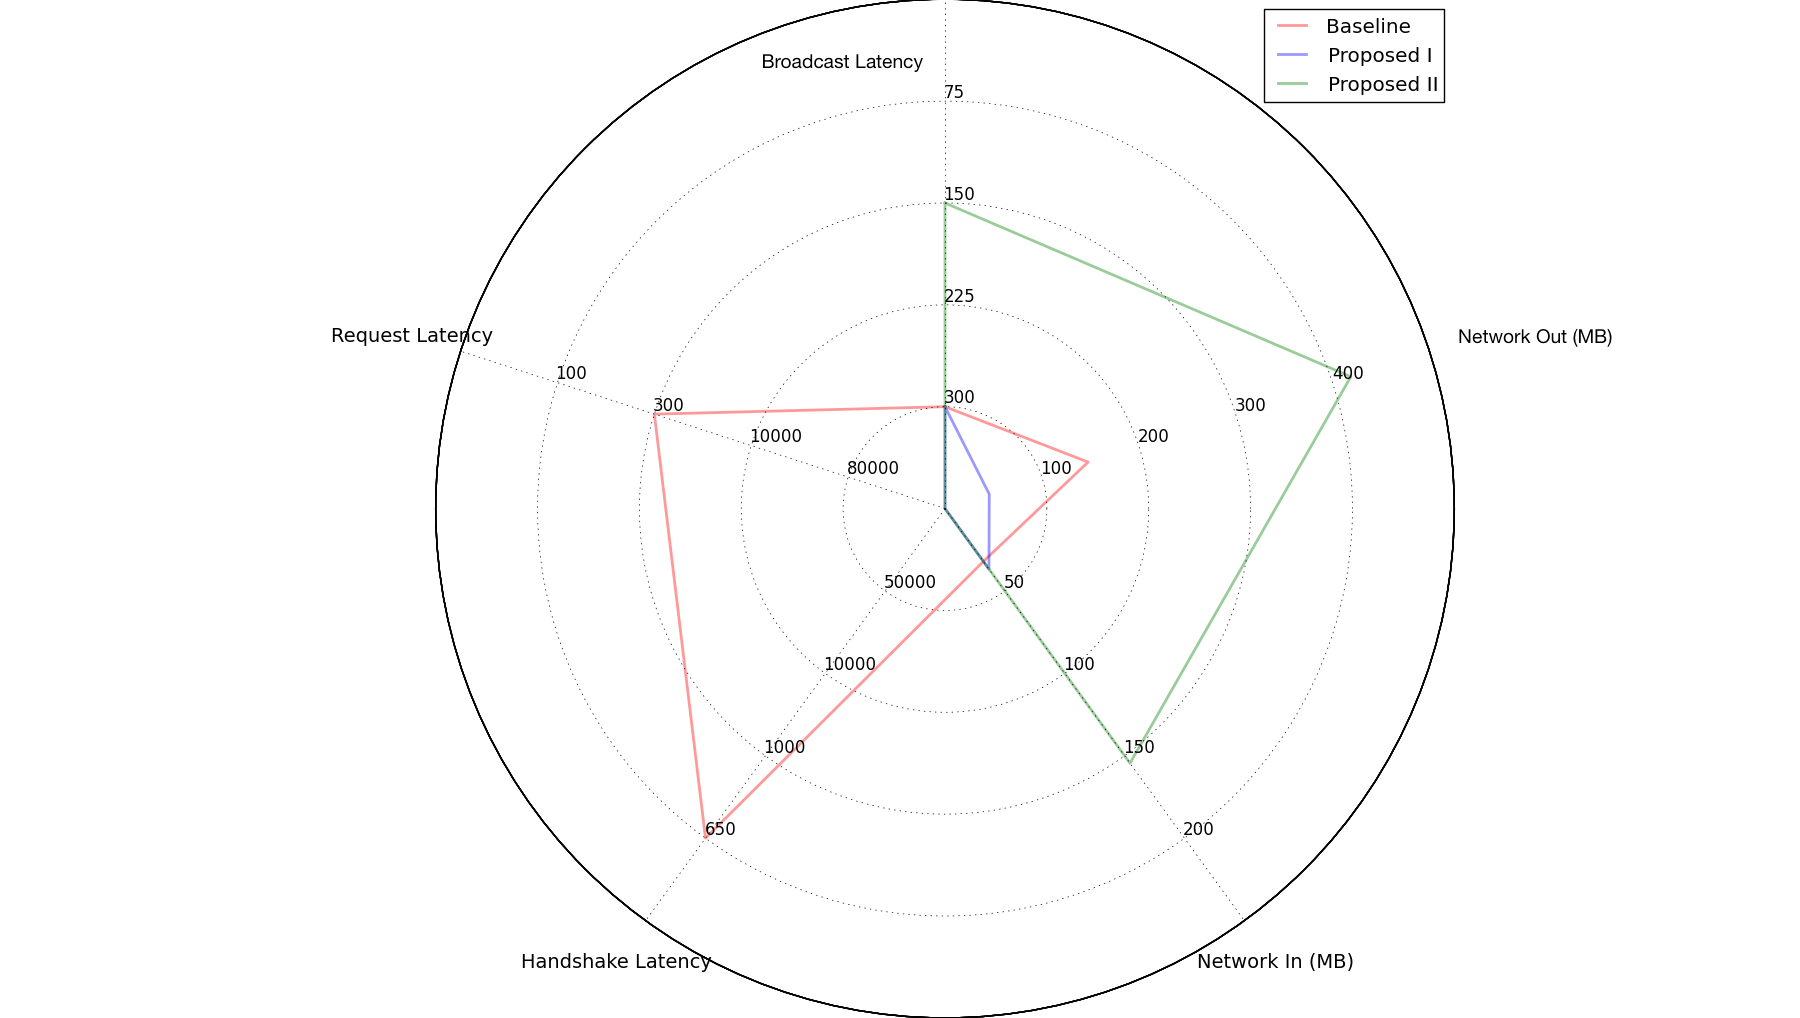
\includegraphics[scale=0.3]{spm}
\caption{System Performance Meter (average values for each architecture, rescaled to fit the plot).}
\label{figure:spm}
\end{figure}

\subsection{System Load}
System load is measured using the System Load Meter. Since all the input values (listed below) are in form of just one, summarizing value, the meter has one value per each architecture setup.

Meter inputs:
\begin{itemize}
  \item \texttt{Successful connections} - number of users who successfully connected to the system (opened a WebSocket connection), summed from all client reports,
  \item \texttt{Handled requests count} - sum of all user requests (send over the WebSocket connection) handled by the system,
  \item \texttt{Redis hits} - number of successful queries directed at redis during the benchmark,
  \item \texttt{MySQL queries} - number of MySQL queries performed during the benchmark run.
\end{itemize}

\begin{table}[H]
\begin{center}
\begin{tabular}{llll}
  \texttt{Value}                & \texttt{Baseline}   & \texttt{Proposed I}  & \texttt{Proposed II} \\
  \hline
  Successful conn.              & 23,999              & 13,023               & 15,767              \\
  Handled requests              & 8,449,173           & 589,923              & 796,660              \\
  Redis hits                    & 50,025,404          & 3,492,791            & 5,513,412              \\
  Redis misses                  & 312,581             & 23,514               & 36,518              \\
  MySQL queries                 & 33,158,053          & 2,343,338            & 3,595,390              \\
  \hline
  \texttt{SLM}                  & \texttt{200.138324} & \texttt{0.14640}     & \texttt{2.199334}         \\
\end{tabular}
\end{center}
\caption{System load (SLM value divided by $10^{12}$).}
\label{table:slm}
\end{table}

The absolute SLM meter value and all the values presented in the table \ref{table:slm} clearly show that the Baseline architecture performs best. In case of system load, it outperforms the proposed architectures, which fail to sustain the load applied during benchmarking, by an order of magnitude \ref{figure:slm}.

\begin{figure}[H]
\centering
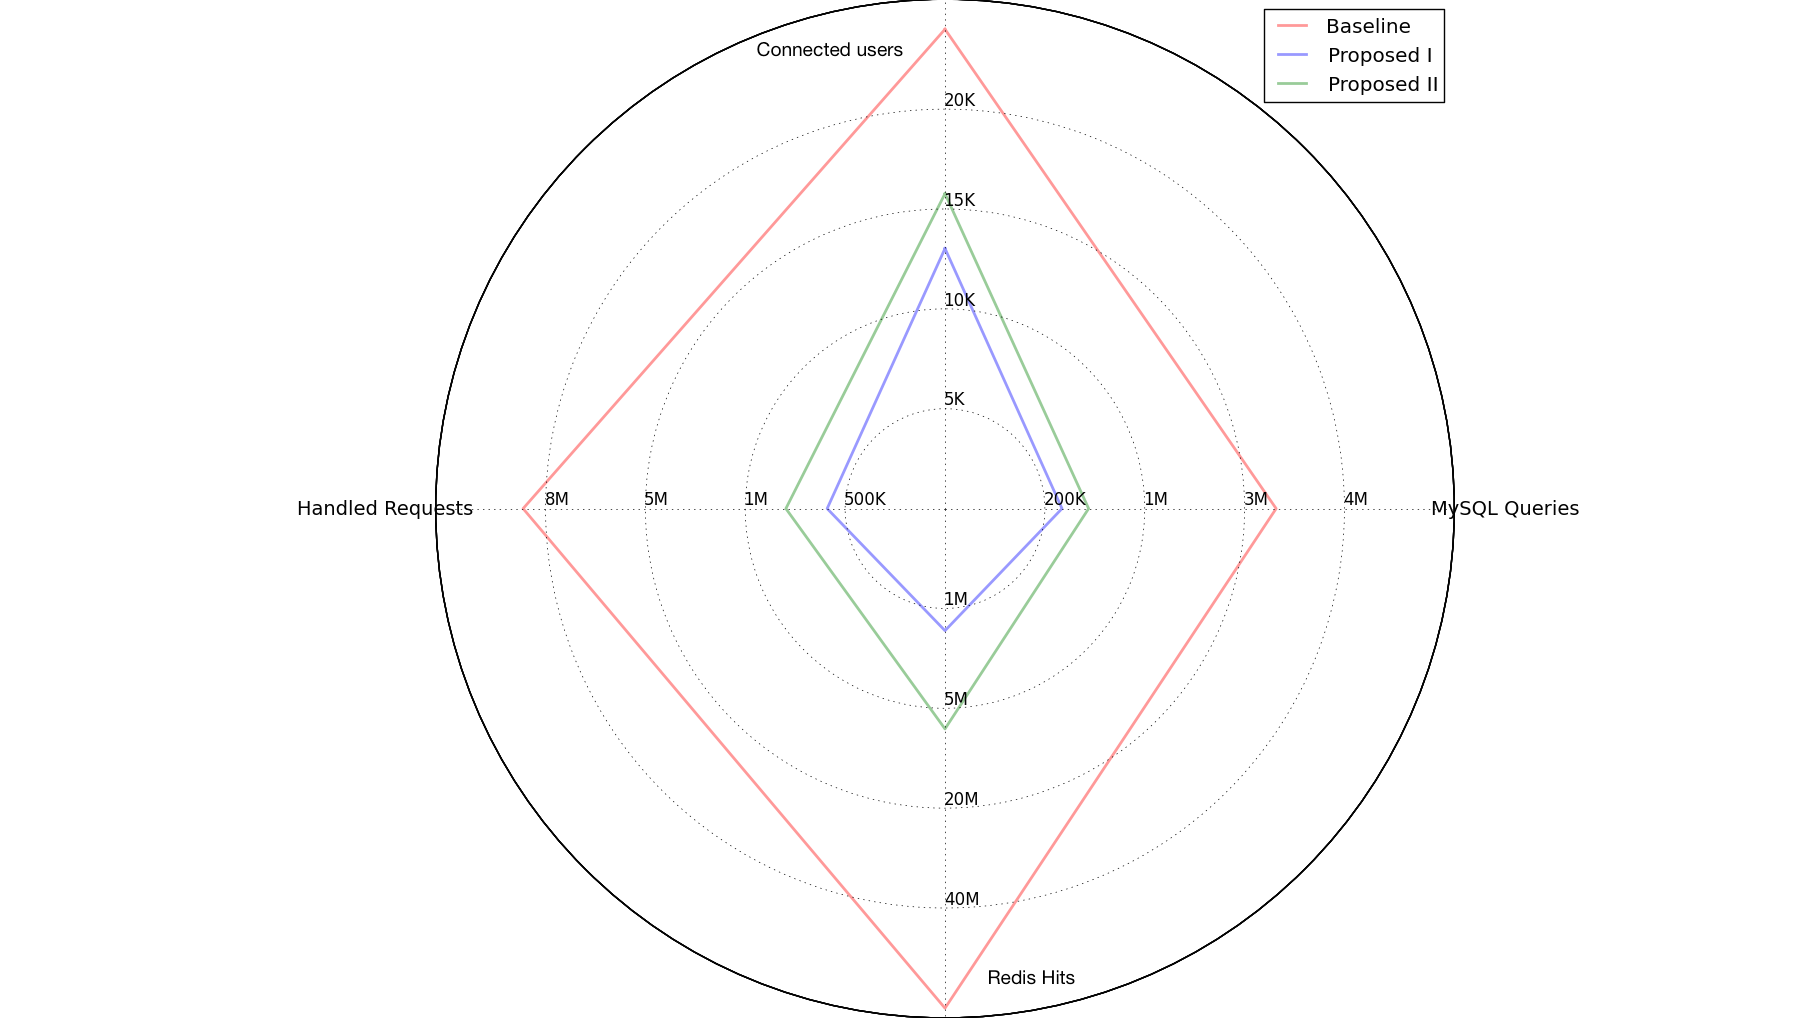
\includegraphics[scale=0.3]{slm}
\caption{System Load Meter (values rescaled to fit the plot).}
\label{figure:slm}
\end{figure}

\subsection{Cost Estimates}

As cost of operating deployed architectures is important to the host organization, I updated the following model (System Effective Capacity) with cost adjustments.

The cost was estimated using only running costs - no setup cost (such as copying AMIs across regions, volume creation) was included in the estimates. All costs are estimated on an hourly basis (since this is the minimum billing period with Amazon); costs specified as monthly rates where brought down to hourly rates assuming 30 days in a month. All outgoing data was assumed to be going out "to the internet", even though different rates apply for Amazon cross-region transfer (which was really the case during benchmarking, but is not in the real-life setup). Where costs differ across regions, Irish prices were applied to simplify the estimation process. The cost of this research, together with preparations and client machines, amounted to around 500\$. Costs computed using Amazon official sources\footnote{\url{http://aws.amazon.com/ec2/pricing/}}\footnote{\url{https://aws.amazon.com/ebs/pricing/}}\footnote{\url{http://aws.amazon.com/rds/pricing/}}.

\begin{table}[H]
\begin{center}
\begin{tabular}{llll}
  \texttt{AWS Service}               & \texttt{Baseline}   & \texttt{Proposed I}  & \texttt{Proposed II}  \\
  \hline
  \texttt{EC2} \\
  Unit hourly cost                   & 1.912               & (0.025;0.0171)       & (0.05;0.0171)         \\
  Units                              & 1                   & (8;1)                & (8+1;1)                 \\
  Total                              & 1.912               & 0.217                & 0.4671                \\
  \hline
  \texttt{EBS Storage} \\
  Unit hourly cost                   & 0.00019             & 0.00019              & 0.00019               \\
  Units                              & 140                 & 140 * (8+1) + 100    & 140 * (8+1) + 100 * 8 \\
  Total                              & 0.026               & 0.253                & 0.3914                \\
  \hline
  \texttt{EBS IOPS} \\
  Unit hourly cost                   & 0.0001              & 0.0001               & 0.0001                \\
  Units                              & 4000                & 4000 * (8+1) + 1000  & 4000 * (8+1) + 1000 * 8 \\
  Total                              & 0.4                 & 3.61                 & 4.4 \\
  \hline
  \texttt{RDS} \\
  Unit cost                          & 0                   & 2.56                 & (0.85;0.09)              \\
  Units                              & 0                   & 1                    & (1;7)                   \\
  Total                              & 0                   & 2.56                 &  1.48                  \\
  \hline
  \texttt{Data In} \\
  Unit cost per GB                   & 0.01                & 0.01                & 0.01              \\
  Units (per hour)                   & 2.91 * 2/3          & 3.37 * 2/3          & 13.88 * 2/3  \\
  Total                              & 0.0194              & 0.02246             & 0.09253  \\
  \hline
  \texttt{Data out} \\
  Unit cost per GB                   & 0.01                & 0.01                & 0.01              \\
  Units (per hour)                   & 13.6951 * 2/3       & 4.19 * 2/3          & 36.81 * 2/3        \\
  Total                              & 0.091               & 0.02793             & 0.2454             \\
  \hline
  \texttt{Detailed monitoring} \\
  Unit cost per hour                 & 0.005               & 0.005               & 0.005              \\
  Units                              & 1                   & 8+1                 & 8+1     \\
  Total                              & 0.005               & 0.045               & .045       \\
  \hline
  \texttt{Route 53} \\
  Total                              & 0                   & 0.014               & 0.014              \\
  \hline
  \texttt{Total Cost}                & \texttt{2.4534} & \texttt{6.74939}     & \texttt{7.13543}         \\
\end{tabular}
\end{center}
\caption{System running cost per hour (all prices in \$).}
\label{table:cost}
\end{table}

As shown in the table \ref{table:cost}, the baseline architecture is the cheapest. It is the simplest and least distributed, this is why it needs least services to support it.

A huge chunk of cost is comprised of EBS, which can be avoided. An AMI on which all the servers are based was originally created with EBS storage of 4000 IOPS (for high performance) and required minimum 140GB of storage. In order to reuse the image, each server needed to be assigned at least that amount of storage, which was otherwise not necessary.

\subsection{System Effective Cost-Adjusted Capacity}
It is measured using System Effective Capacity Meter extended with the cost factor. The inputs to the meter are the following:
\begin{itemize}
  \item \texttt{System Load Meter output} - with values reduced by $10^{12}$,
  \item \texttt{System Performance Meter output} - with minimum, average and maximum values,
  \item \texttt{Computing Resource Utilization Meter} - with minimum, average and maximum values,
  \item \texttt{Cost} - how long a system can run on 1\$, so $1/hourlyTotalCost$ (computed in the previous section) is input.
\end{itemize}

\begin{table}[H]
\begin{center}
\begin{tabular}{llll}
  \texttt{Metric}               & \texttt{Baseline}   & \texttt{Proposed I}  & \texttt{Proposed II}  \\
  \hline
  SLM                           & 200.193             & 0.14640              & 2.19933         \\
  \hline
  SPM min                       & 130.46082           & 0.23341              & 6.79360                 \\
  SPM avg                       & 2251.88501          & 797.62981            & 30771.49954                 \\
  SPM max                       & 6368.43238          & 1029.5834            & 43476.89380                 \\
  \hline
  CRUM min                      & 56.82622            & 24.74547             & 29.71976                \\
  CRUM avg                      & 298.30941           & 63.04514             & 74.87883                 \\
  CRUM max                      & 414.57287           & 69.02704             & 85.63872                 \\
  \hline
  Hours on 1\$                 & 1/2.4534             & 1/6.74939            & 1/7.13543                \\
  \hline
  \texttt{SEC min}              & 16,814.25           & 4.75                 & 110.66         \\
  \texttt{SEC avg}              & \texttt{561,317.23} & \texttt{27,592.52}   & \texttt{1,185,910.70}         \\
  \texttt{SEC max}              & 1,957,497.59        & 35,615.04            & 1,909,469.13         \\
\end{tabular}
\end{center}
\caption{System cost-adjusted effective capacity.}
\label{table:sec}
\end{table}

Again, second proposed architecture achieves the best result according to the SEC meter so the results need to be taken in with a grain of salt \ref{table:sec}. This is the propagated consequence of the high performance meter values for this architecture caused by high data transfers.

\begin{figure}[H]
\centering
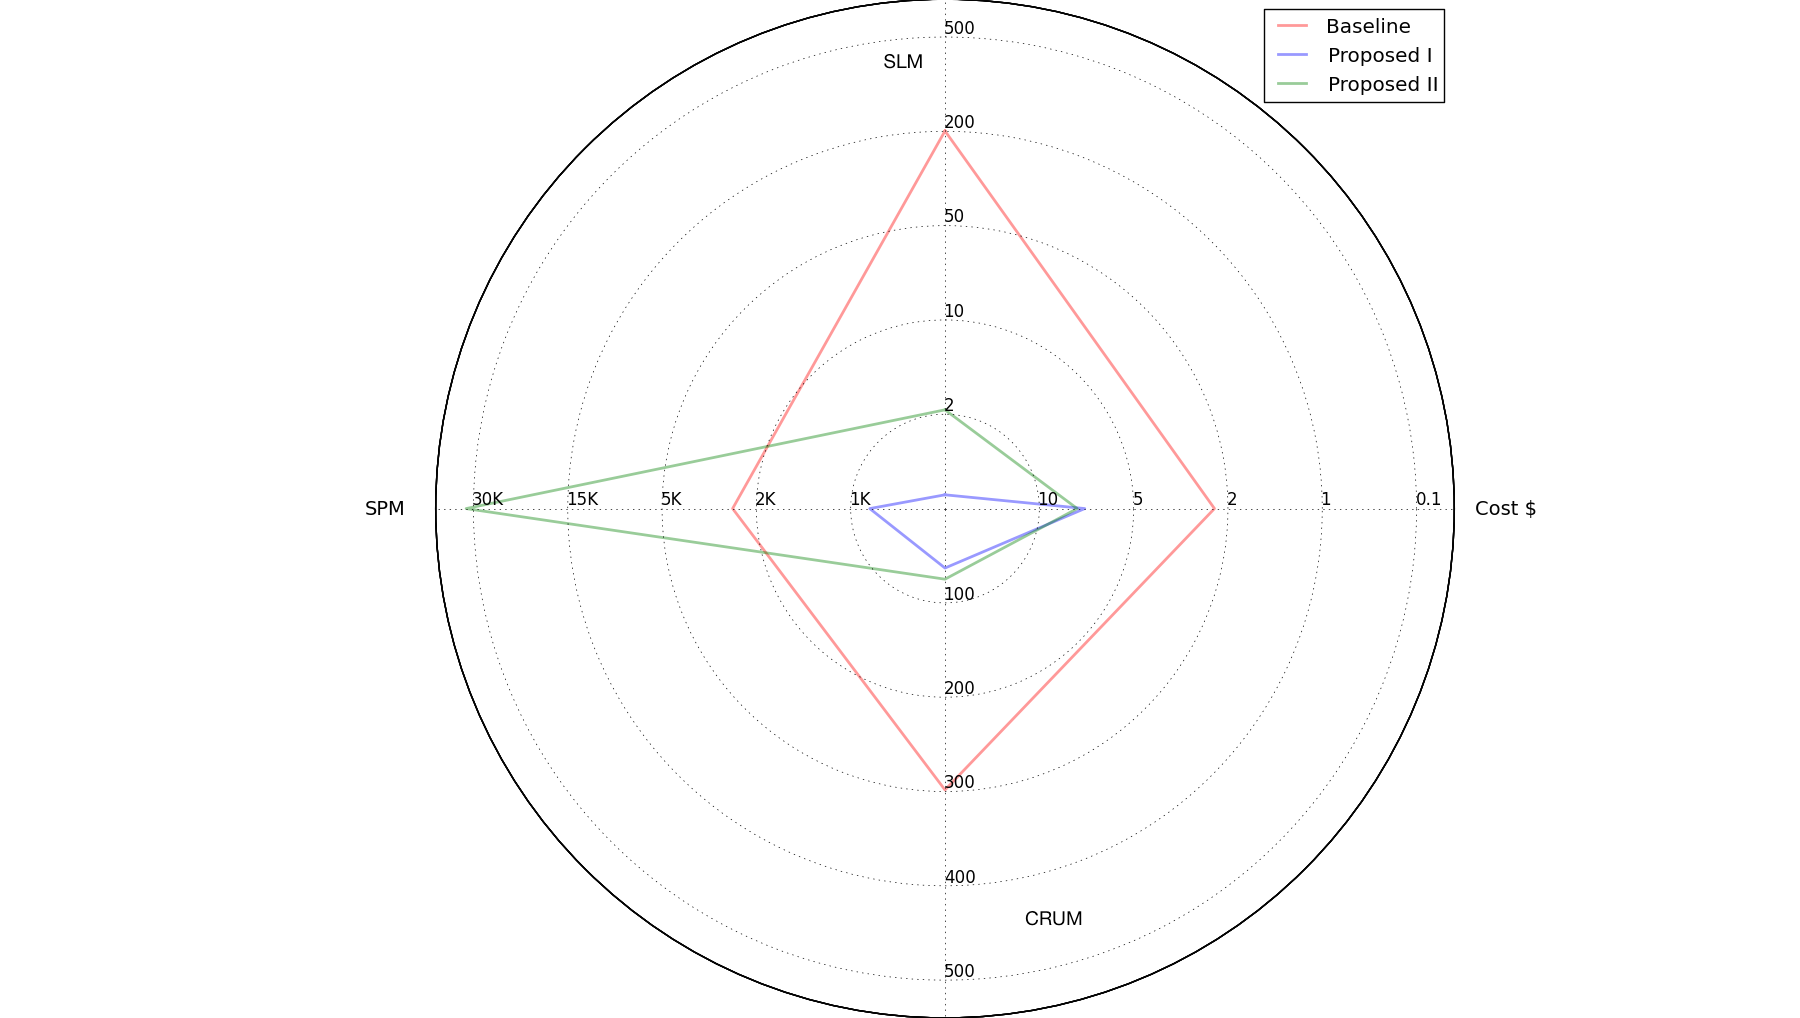
\includegraphics[scale=0.3]{secplot}
\caption{System Effective Capacity Meter (values rescaled to fit the plot).}
\label{figure:secplot}
\end{figure}

\subsection{Effective Scalability}
I apply a change to the original model. Since I do not have a range of System Load Meter values, I use System Performance Meter values instead.

\subsubsection{Effective System Scalability}
I compute the Effective System Scalability as follows:

$$ESS = (SPM_{max} - SPM_{min}) / (SEC_{max}-SEC_{min})$$

\begin{table}[H]
\begin{center}
\begin{tabular}{llll}
  \texttt{Metric}               & \texttt{Baseline}   & \texttt{Proposed I}  & \texttt{Proposed II}  \\
  \hline
  SPM min                       & 130.46082           & 0.23341              & 6.79360                 \\
  SPM max                       & 6368.43238          & 1029.5834            & 43476.89380                 \\
  \hline
  SEC min                       & 16,814.25           & 4.75                 & 110.66         \\
  SEC max                       & 1,957,497.59        & 35,615.04            & 1,909,469.13         \\
  \hline
  \texttt{ESS}                   & \texttt{0.00321}     & \texttt{0.0289}      & \texttt{0.02277}
\end{tabular}
\end{center}
\caption{Effective System Scalability.}
\label{table:ess}
\end{table}

Contrary to original expectations, the model does not provide useful insight to the performance of architectures. It informs about the difference between top and worst performance of each architecture.

It also shows that models are rather sensitive to input values. For instance, the increased internal transfer in Proposed architecture II strongly influences all the derivative models based on System Performance Meter.

The model could more useful when different loads are applied on the same architecture.

\section{General Interpretation}

According to all primary metrics Baseline architecture performs best, followed by the 2nd proposed architecture and the 1st proposed architecture performing worst.

The cause of such state of affairs is the combination of WebSocket server technology and database drivers that are used in the tested system \ref{The System Under Test}. The System runs Tornado, which is single-threaded. Without fully asynchronous and non-blocking I/O operations, system scalability is severely limited. Our database drivers have proven not to be fully non-blocking, which seems like a foreseeable thing, and yet it wasn't discovered until the benchmark runs. The issue only manifests itself when data source is not located in server's proximity. This is when network latencies are added to each database query and, because of that, request handling times escalate.

A sample use case demonstrates the behavior: 1000 users connecting from Sydney to Ireland at the same time. Let us assume a latency of the Sydney-Ireland round-trip to be 1000ms, and the database query handling time to be 1ms.

If the server is connected in the same data center as the database (as is the case in baseline architecture), all users arrive at the same time (more or less). First user's request is handled in 1ms, second user's in 2ms (the 1st millisecond was used for handling the 1st user's query, the server process was blocked), third user in 3ms and so on. On average, the thousand users are server with a latency of ~1500ms (1000ms for a Sydney-Ireland round-trip) and 500ms as an average time before the database query can run (best case scenario is 1ms, worst case 1000ms). After 1000ms, the server has finished serving all the requests, and if another 1000 arrive next second, it will handle all of them too. This is a sustainable setup. This case is depicted on figure \ref{figure:case1}.

\begin{figure}[H]
\centering
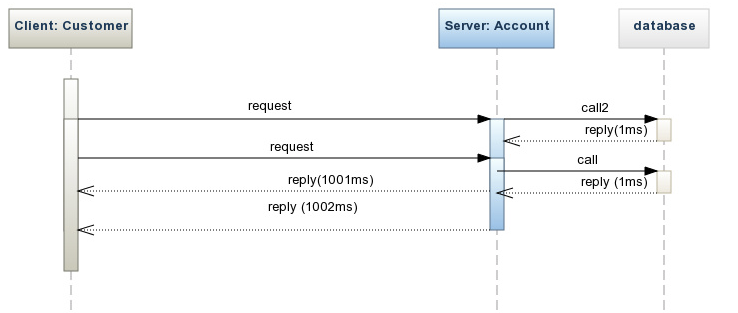
\includegraphics[scale=0.5]{case1}
\caption{Baseline architecture case.}
\label{figure:case1}
\end{figure}

When the server is moved to Sydney, but the data source stays in Ireland, the flow is changed. When 1000 users send a request at the same time, all of them arrive at their local server (let's assume) instantly. First user is served in 1001ms (1ms database query + 1000ms roundtrip latency), second user is served in 2001 ms (initial 1000ms the server was blocked for the first user's blocking database query), third user in 3001 ms, etc. On average, the thousand users are served with a latency of around \texttt{500,000ms}. And this is just for the first round of requests. If another 1000 arrive at the second second, the latencies experienced by these users will be even higher. This case is depicted on figure \ref{figure:case2}. This is obviously not sustainable, yet this is the setup proposed architectures introduced - II proposed architectures to a lesser extent, since only database writes were done on a remote database, reads were performed on a local replica.

\begin{figure}[H]
\centering
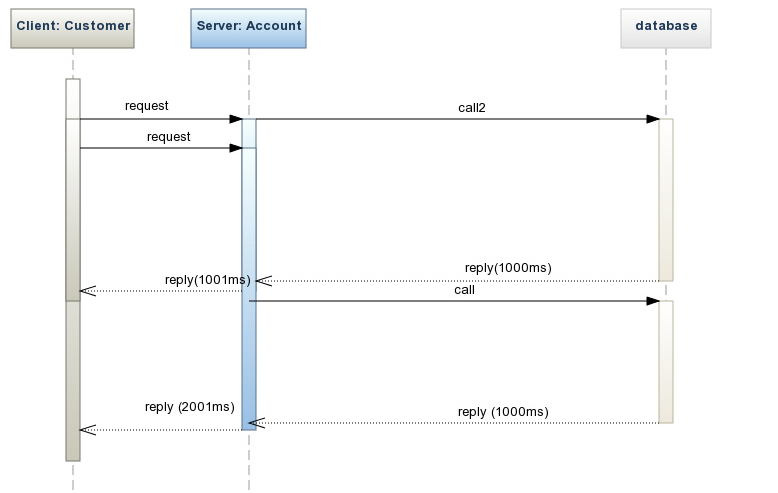
\includegraphics[scale=0.5]{case2}
\caption{Proposed architectures case.}
\label{figure:case2}
\end{figure}
An attempt was made to replace the database drivers, yet this is no trivial task. One cannot simply code asynchronicity around the intrinsically synchronous calls. Nevertheless, the drivers were fully replaced with asynchronous ones, but another issue cropped up when this was performed.

The server was now capable of serving users in an asynchronous manner, provided that there was no more than one asynchronous operation in each execution flow. Unfortunately, this is not always the case with the tested system. Listing \ref{lstlisting:async} explains the 3 cases: fully-synchronous, asynchronous working and asynchronous not working entirely as intended.

\begin{sourcecode}[H]
\begin{lstlisting}[style=mono, language=Python]
# WebSocketHandler class

# synchronous
def handle_message(self, message):
    value = self.db(get_value)
    # the whole process is blocked until the query above returns
    return self.write(value)

# asynchronous working
@tornado.gen.engine
@tornado.web.asynchronous
def handle_message_async(self, message, callback):
    value = yield tornado.gen.Task(self.db, get_value)
    # execution of the flow stops here, but is not blocking the process
    # other users are served at the same time
    callback(self.write, value)

# asynchronous not fully working
@tornado.gen.engine
@tornado.web.asynchronous
def handle_message_async(self, message, callback):
    value   = yield tornado.gen.Task(self.db, get_value)
    # execution of the flow stops here, but is not blocking the process
    value_2 = yield tornado.gen.Task(self.db, get_value_2)
    # execution of the flow stops here, but is not blocking the process
    # the two calls above WILL NOT be executed in parallel
    # that means that each user request handling latency is multiplied
    # the number of db queries - still unsustainable.
    callback(self.write, value, value_2)
\end{lstlisting}
\caption{Synchronous vs Asynchronous Tornado.}
\label{lstlisting:async}
\end{sourcecode}

The reason why multiple yields cannot work in parallel is the following. The lines 13, 22 and 24 of the listing \ref{lstlisting:async} show the execution of so called coroutines. If a coroutine (\textit{self.db.get\_value}) does not \textit{yield} from the inside (and it does not, since if performs an atomic I/O-bound operation), there is no way for the coroutine scheduler to interleave the calls and run them in parallel. That's the whole point of coroutines: they're cooperative, not preemptive.

It is possible to make the architecture work on a current technology stack even with remote data sources, yet no more than one database query can be performed per each message handling. Queries should therefore be batched, and that requires major application code changes.

\section{Additional Observations}

\subsection{Latencies by region}
As table \ref{table:regionlats} shows, the differences between regions are observable in each of the architectures. In all cases, most servers (and writable database masters) are located in Ireland's data center. One can observe on figure \ref{figure:latgeo} that the bigger the geographical distance between clients location and Ireland, the bigger the latencies.

\begin{table}[H]
\begin{center}
\begin{tabular}{llll}
  \texttt{Region}               & \texttt{Baseline}   & \texttt{Proposed I}  & \texttt{Proposed II}  \\
  \hline
  \texttt{Handshaking} \\
  Ireland                       & 19                  & 452                  & 348                 \\
  N. Virginia                   & 319                 & 1162379              & 291177                 \\
  Oregon                        & 574                 & 1998393              & 585971                 \\
  California                    & 633                 & 1932505              & 707331                 \\
  Sao Paulo                     & 818                 & 1884244              & 958826                 \\
  Singapore                     & 858                 & 2131407              & 942381                 \\
  Tokyo                         & 877                 & 1981380              & 1002561                 \\
  Sydney                        & 1269                & 1857882              & 1655476                 \\
  \texttt{Global}               & \texttt{671}        & \texttt{1549675}     & \texttt{733047}                 \\
  \hline
  \texttt{Request Handling} \\
  Ireland                       & 128                 & 8147                 & 3932                 \\
  N. Virginia                   & 205                 & 640398               & 522244                 \\
  Oregon                        & 272                 & 1084066              & 732814                 \\
  California                    & 284                 & 1160773              & 765508                 \\
  Sao Paulo                     & 330                 & 992451               & 815666                 \\
  Singapore                     & 325                 & 1184645              & 812563                 \\
  Tokyo                         & 347                 & 1319677              & 846521                 \\
  Sydney                        & 441                 & 1556088              & 938513                 \\
  \texttt{Global}               & \texttt{291}        & \texttt{90987}       & \texttt{82595}                 \\
  \hline
  \texttt{Broadcast} \\
  Ireland                       & 223                 & 96                   & 107                 \\
  N. Virginia                   & 287                 & 126                  & 114                 \\
  Oregon                        & 268                 & 419                  & 145                 \\
  California                    & 296                 & 440                  & 147                 \\
  Sao Paulo                     & 322                 & 588                  & 168                 \\
  Singapore                     & 315                 & 542                  & 156                 \\
  Tokyo                         & 327                 & 587                  & 176                 \\
  Sydney                        & 379                 & 829                  & 217                 \\
  \texttt{Global}               & \texttt{302}        & \texttt{293}         & \texttt{141}                 \\
\end{tabular}
\end{center}
\caption{Weighted average latencies (in ms) reported by clients, grouped by region.}
\label{table:regionlats}
\end{table}

\begin{figure}[H]
\centering
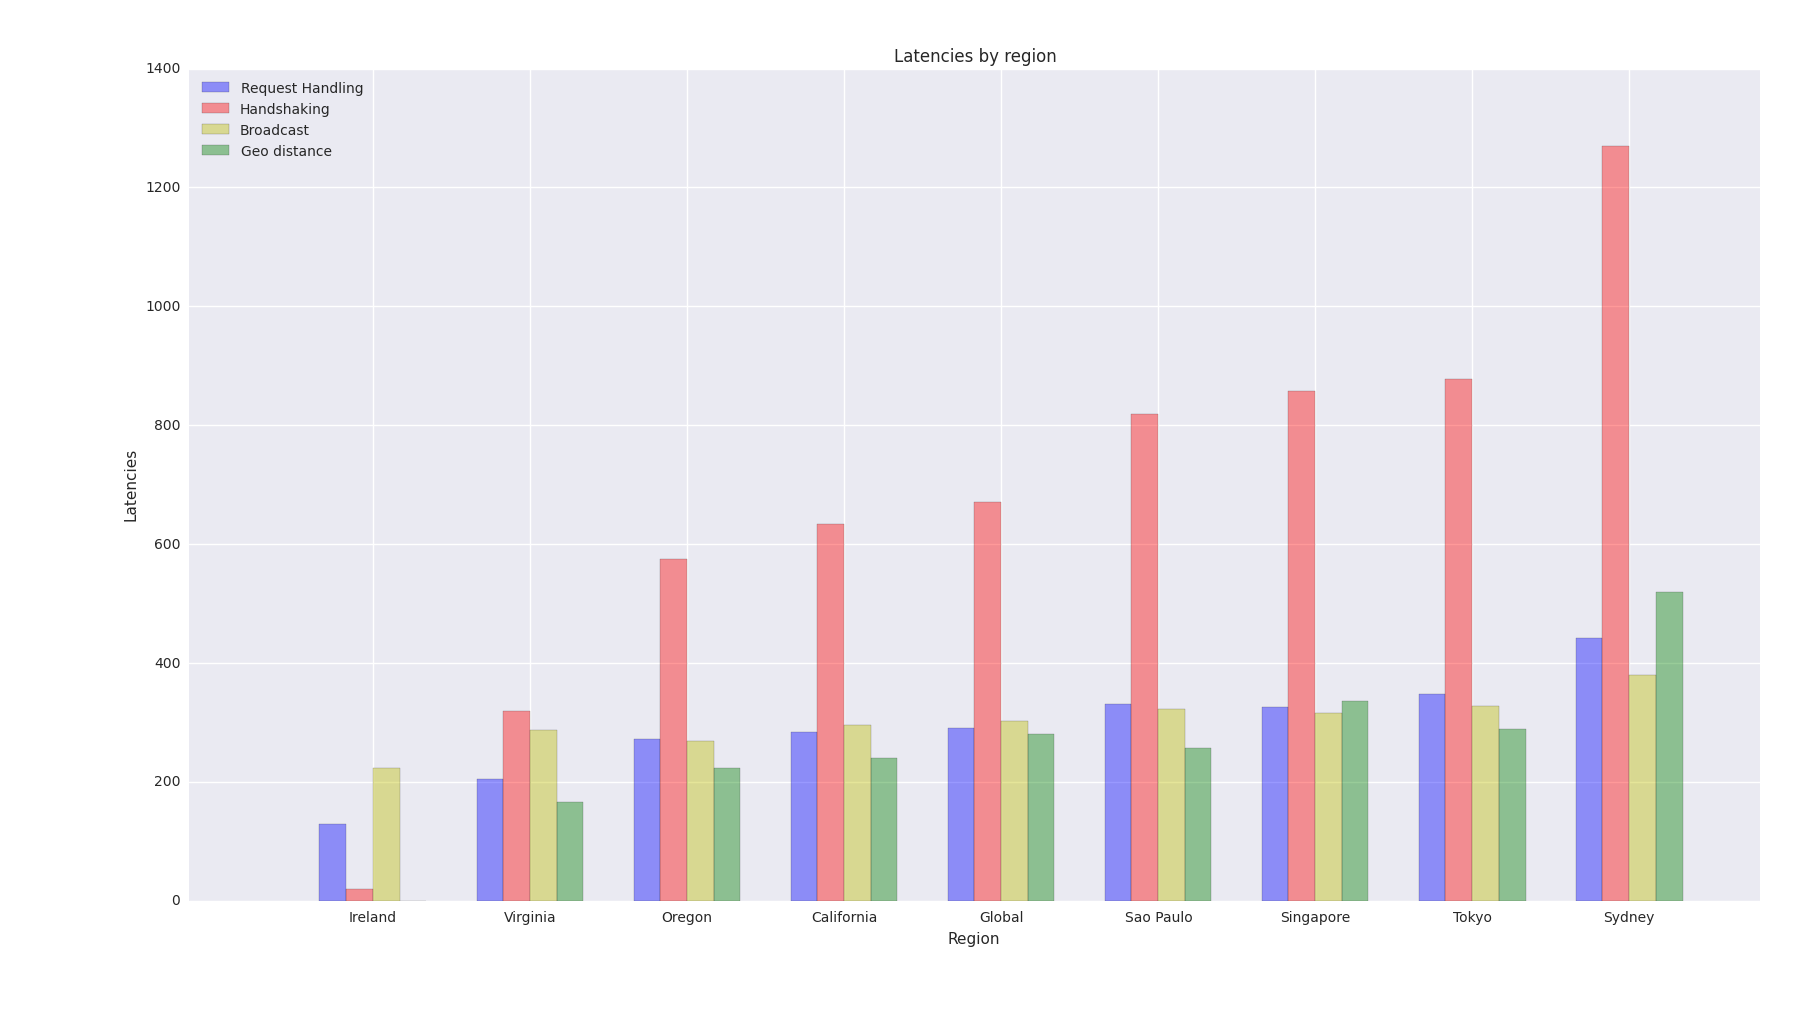
\includegraphics[scale=0.3]{latgeo}
\caption{Latencies by region (geographic distance in km, rescaled).}
\label{figure:latgeo}
\end{figure}

Depicted geographic distance on figure \ref{figure:latgeo} is measured between Ireland and a city/state of a given data center. Global uses an average of all others. Latencies are taken from the results of the benchmark run against the baseline architecture.

\subsection{TCP vs CPU}
% splitting up redis and MySQL onto separate instances causes CPUs to max out 100\% (handling the networks stack?) and data traffic to spike (obvsly)

% backup by table from lab notes 21.07

%%%%%%%%%%%%%%%%%%%%%%%%%%%%%%%%%%%%%%%%%%%%%%%%%%%%%%%%%%%%%%%%%%%%%%%%%%%%%%%%
\chapter{Conclusions and Evaluation}\label{Conclusions and Evaluation}
%%%%%%%%%%%%%%%%%%%%%%%%%%%%%%%%%%%%%%%%%%%%%%%%%%%%%%%%%%%%%%%%%%%%%%%%%%%%%%%%
\epigraph{"Nine women can't make a baby in one month."}{--- Fred Brooks, The Mythical Man-Month}

\section{Short Summary}
In this research, a load test suite generating an arbitrary load over an arbitrary period of time according to the customizable messaging scenarios and user distributions has been designed and implemented. Metric collection for the client test suite and all system components has also been put in place. Multiple bottlenecks of the system have been identified and optimizations proposed and applied. Different architecture decompositions of the system \ref{The System Under Test} were proposed and tested with a benchmark utilizing the load test suite. Metrics have been collected, aggregated and a comparative, quantitative analysis of architectures has been performed.

\section{Research Questions and Hypothesis}
\subsection{Research Questions}
\textit{The research questions put forward in the introduction are the following:
\begin{enumerate}
  \item What's the architecture decomposition stack that:
    \begin{enumerate}
      \item guarantees data delivery to geographically distributed users with minimal, consistent and manageable latency?
      \item guarantees lowest cost and best degree of utilization of the employed resources within a data center?
    \end{enumerate}
  \item Does architecture with geographical awareness of its users' distribution provide better Quality of Service than the baseline architecture?
\end{enumerate}}

The research has yielded the following answers:
\begin{enumerate}
  \item The baseline architecture \ref{Baseline Architecture} performs better than the proposed architectures \ref{Proposed Architecture I} \ref{Proposed Architecture II} with regard to all analyzed aspects of the system.
  \item The distribuetd architectures \ref{Proposed Architecture I} and \ref{Proposed Architecture II} do not provide better Quality of Service than the baseline architecture \ref{Baseline Architecture}.
\end{enumerate}

\subsection{Hypothesis}
\textit{The correct geographical decomposition of the stack of The System Under Test \ref{The System Under Test} can lead to improved performance in comparison with the Baseline Architecture \ref{Baseline Architecture}.}

The hypothesis is refuted in the research, the Baseline Architecture \ref{Baseline Architecture} performed better than the proposed improvements \ref{Proposed Architecture I} and \ref{Proposed Architecture II}.

What needs to be emphasized that the answers and rebuttal of the hypothesis result from the inherent system limitations identified in this research. They are based on the every tested state of the system, yet they might not hold true anymore if the existing known limitations are overcome.

\section{Other conclusions}
As the research progressed, I have to multiple conclusions that might not be directly related to the research question but I believe are worth bringing up nevertheless:
\begin{description}
  \item[Building a scalable system] - this is fairly common knowledge, but in order to be scalable the system needs to be designed in a way that facilitates that from the start. State should be concentrated in a layer that has good scalability mechanisms and all other system nodes should hold as little (or none at all) state as possible. This guarantees they can be dynamically added to and removed from the system. One cannot simply add a scalability module which will drastically improve the performance of the system at scale. It is a process of digging deeper and obtaining a better understanding of the system architecture and technologies used and applying that knowledge to a scalable design. It is important to set scalability goals that the system should satisfy, otherwise the process can go on forever.
  \item[Hardware does not have to be the limit] - in the case of the tested system, resource utilization (as the metrics show) is fairly low. The operating system has been tuned to facilitate system's needs; if this is done properly, suboptimal utilization of some kind of resource or a suboptimal programming/architecture solution is most likely the limit to scalability. I am willing to jump to a conclusion that this holds true for most software systems.
  \item[Deploying in the cloud] has proved to be much more challenging than expected. The distributed setup is significantly different from a simple, centralized one. One should be prepared to familiarize themselves thoroughly with the details of the cloud solution used in a process of preparing the system for deployment in the cloud.
  \item[Focus on achieving the predefined goals] - it is to get lost in trying to optimize irrelevant aspects of the architecture (guilty as charged). I have spent days making sure that the kernel is tuned so that thousand of users can connect simultaneously to find out later that our system can only sustain values order of magnitude smaller.
  \item[AWS Cloud stack is not built for global setups] - at least for global setups that our system requires. A lot of functionality (elasticache, elastic load balancing, auto scaling) is limited to one region. If the same setup needs to be replicated in different regions, the whole process needs to be performed manually (or using AWS API, but still this proved to be time-consuming).
  \item[Publishing user-generated content globally] - this needs to be performed with some degree of sensibility. If users generate content hundred times a second, it is not feasible (nor reasonable) to broadcast all updates to all users. They probably do not need to see all of them in real time. Some form of batching can be really helpful and can reduce amount of data sent by orders of magnitude.
  \item[Read replication] - provides only some improved scalability. If the application is write-intensive (as is the tested system), this is not the best solution.
  \item[Data Locality] - is extremely important. There is no way to beat the speed of light (and in most cases internet middle-man introduced overhead); one needs to make sure that the data retrieval mechanisms in the \texttt{stateless} servers are fully asynchronous and non-blocking or that a sufficient number of threads can be supported. Otherwise, at a big enough scale, a catastrophy will ensue.
\end{description}

% \section{Statistical Significance}
% http://technology.stitchfix.com/blog/2015/05/26/significant-sample/
% http://insightdatascience.com/blog/ab\_testing\_statistics.html
% http://www.qubit.com/sites/default/files/pdf/mostwinningabtestresultsareillusory\_0.pdf
% http://www.evanmiller.org/how-not-to-run-an-ab-test.html

\section{Threats to validity}
Following threats to validity have been identified:
\begin{itemize}
  \item Cloud computing environments, such as EC2, are outside of the researcher's control. They can only be monitored and influenced to an extent. Since it is a shared environment, it is hard to predict how other systems that the deployed system is sharing resources with will behave (e.g they might end up under a DDOS attack).
  \item Global network conditions are inherently non-deterministic, the benchmark might (and probably would) yield different results if performed e.g. during a Superbowl or World Cup final.
  \item Because of the system limitations, I am not able to make any claims about other, truly asynchronous systems.
\end{itemize}

\section{Host Company Benefits}
Even though primary question has only been answered in scope of current system limitations, the research has already yielded multiple benefits for the host company (and hopefully will continue doing so):
\begin{itemize}
  \item Massive systems bottlenecks have been introduced, solutions designed and implemented.
  \item Measurement and load test suite can be used in the future to benchmark further architecture improvements.
  \item A Baseline for further tests has been established; now, when a company switches to some other data solution (such as DynamoDB), there is a way to verify if the promised improvement is actually hapenning.
  \item A real-time telemetry has been added to the system. The distributed servers report metrics that can be viewed in real time.
  \item A cloud orchestration suite has been implemented - whenever a system architecture changes, the tools to deploy the updated architecture are available.
\end{itemize}

%%%%%%%%%%%%%%%%%%%%%%%%%%%%%%%%%%%%%%%%%%%%%%%%%%%%%%%%%%%%%%%%%%%%%%%%%%%%%%%%
\chapter{Further Work}\label{Further Work}
%%%%%%%%%%%%%%%%%%%%%%%%%%%%%%%%%%%%%%%%%%%%%%%%%%%%%%%%%%%%%%%%%%%%%%%%%%%%%%%%

The scalability of the System Under Test \ref{The System Under Test} is not at a level that satisfies business goals, yet. The journey that was started at literally 25 users continues. The system currently sustains loads in order of tens of thousands, the desired number is around ten million. This will probably require major architectural changes and has been therefore ruled outside of scope for this research.


The benchmark is planned to be reused with varying user distributions per region. This is a natural consecutive step having established system's behavior in basic cases.

A plan exists to test different database technologies - DynamoDB of AWS offering and custom setup of redis and MySQL clusters. A baseline against which to compare this data solutions within our system already exists.

Finally, improvements to the used scalability models could be introduced so that the meter inputs can be weighted in order to reflect researcher's preferences. This could guarantee that they are not that sensitive to single values that influence the meter and its derivatives.
%%%%%%%%%%%%%%%%%%%%%%%%%%%%%%%%%%%%%%%%%%%%%%%%%%%%%%%%%%%%%%%%%%%%%%%%%%%%%%%%
%%%%%%%%%%%%%%%%%%%%%%%%%%%%%%%%%%%%%%%%%%%%%%%%%%%%%%%%%%%%%%%%%%%%%%%%%%%%%%%%
%%%%%%%%%%%%%%%%%%%%%%%%%%%%%%%%%%%%%%%%%%%%%%%%%%%%%%%%%%%%%%%%%%%%%%%%%%%%%%%%

{%\tiny
\bibliographystyle{alphaurl}
\bibliography{thesis}
}

\end{document}
